\documentclass[./main_en.tex]{subfiles}
\graphicspath{{\subfix{./figs}}}

% ------------ main document ------------ 
\begin{document}

\chapter{\chapHydroEn} \label{chap:hydrology}

% custom paragraph skip
\setlength{\parskip}{0mm}

\epigraph{\small{The assertion or assumption that all rises are caused by surface runoff has persisted in articles and even in some hydrology textbooks, despite much evidence to the contrary in forestry and agricultural research.}}{Hewlett \& Hibbert (1967, p. 275) \cite{Hewlett1967}}

\epigraph{\small{A box, objectively defined by distinct dynamics of groundwater, soil solution chemistry, or isotopic composition, with defined area, depth, and porosity, is a much better modeling building block than a myriad of elements in landscapes that are notoriously heterogeneous both vertically and laterally!}}{Jeffrey McDonnell (2003, p. 1872) \cite{Mcdonnell2003a}}

% custom paragraph skip
\setlength{\parskip}{\myparskip}

\section{Zero-order Basins} \label{sec:hydro:intro}

\par \textbf{\gls{hydrology}} is the science that studies continental waters, seeking to understand how water is distributed on continents after precipitating from the atmosphere and before returning to the oceans \cite{chow1964}. In other words, \gls{hydrology} investigates how the \textbf{\gls{hydro_cicle}} manifests in its terrestrial phase, in contrast to Meteorology (which focuses on the atmosphere) or Oceanography (which studies the oceans). When contemplating this, it is easy to imagine large rivers, such as the Amazon and Paraná, as well as other notable rivers like the Danube, Nile, Yellow, Indus, Ganges, and Mississippi. In the case of Brazil, images of lush nature arise, including the vast Amazonian and Pantanal floodplains, as well as the spectacular Iguaçu Falls. Visions related to large-scale human intervention also emerge, such as the hydroelectric complex, with its dams spread throughout the country, and the major transposition and irrigation projects, exemplified by the reservoirs in the Cantareira Mountains, the transposition of the São Francisco River, and the central pivots in the São Marcos River basin. The recent floods that devastated the cities located in the river valleys of Rio Grande do Sul also illustrate that rivers are crucial not only for energy and food production but also for ensuring the basic health and physical safety of the inhabitants of vast urban metropolises. In this regard, it is not uncommon for textbooks on \gls{hydrology} to mention how the first city-states, which emerged in Mesopotamia and Egypt, developed an almost symbiotic relationship with large rivers and their floodplains. Water and society are closely linked.

\begin{figure}[t!] 
\centering				
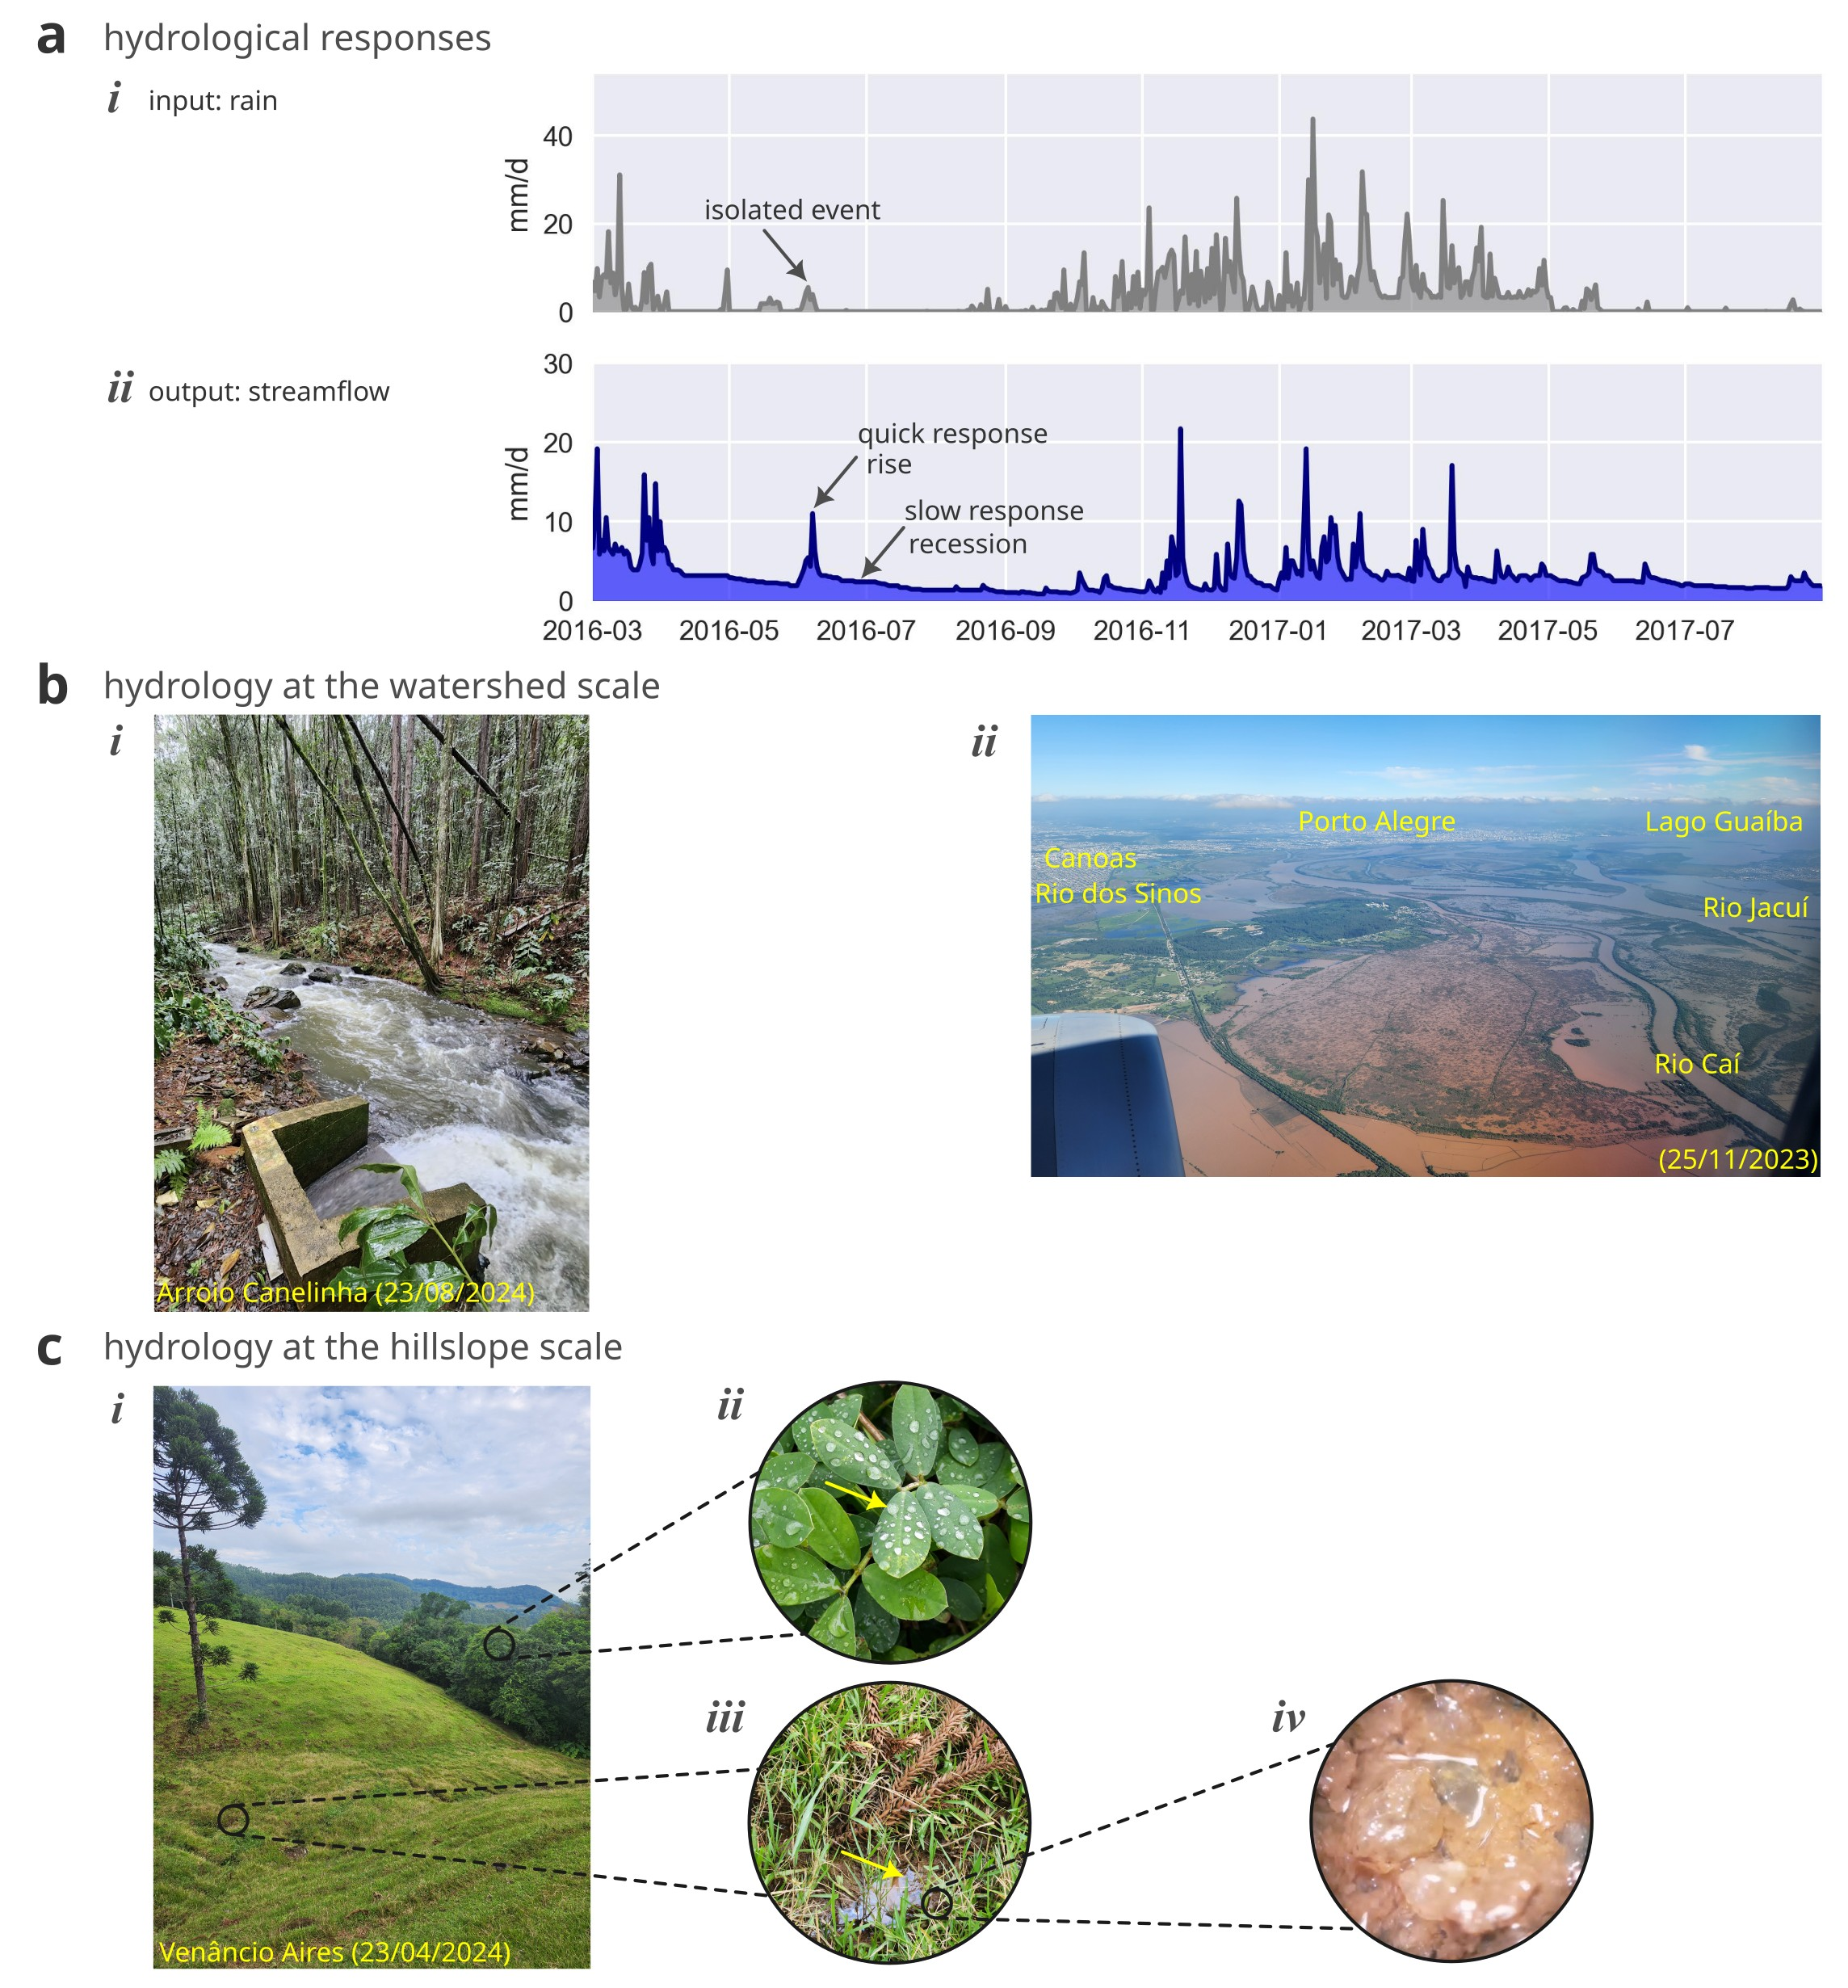
\includegraphics[width=0.98\linewidth]{figs/fig_zero_en.jpg}		
\caption[Hillslopes: where it all begins]
{\textbf{---\;Hillslopes: where it all begins.}
    The most intuitive scale when thinking about hydrological processes is the flow of water in rivers, which are channels that drain water to the ocean. However, the hydrological responses to rainfall events originate in the slopes, in zero-order basins, where rain interacts with the landscape.\;\textbf{a}\;---\;The alternation between fast responses (rises, detail \textrm{\textit{i}}) and slow responses (recessions, detail \textrm{\textit{ii}}), observed in a medium-sized drainage area in the Paraíba do Sul basin (342 km², Rio de Janeiro). Daily rainfall obtained from \texttt{INMET 83738} Station (Resende) and daily flow obtained from \texttt{ANA 58287000} Station (Rialto).\;\textbf{b}\;---\;The evident hydrological processes at the basin scale include the propagation of flow through the drainage network, downhill (detail \textrm{\textit{i}}) and the flooding of plains, when river flow exceeds the larger section of the channels, invading adjacent dry lands (detail \textrm{\textit{ii}}).\;\textbf{c}\;---\;The water that supplies river flow comes from the interaction of rain with the slopes (detail \textrm{\textit{i}}), resulting in surface processes (such as \gls{interception}, in detail \textrm{\textit{ii}}) and subsurface processes (such as soil saturation, details \textrm{\textit{iii}} and \textrm{\textit{iv}}). 
}
\label{fig:hydro:intro} 		
\end{figure}

\par This intuitive interpretation of \gls{hydrology}, however, results from two particular perceptions. The first is the \textbf{\gls{bias-engineer}} that permeates \gls{hydrology}, which has always been marked by a \textbf{\gls{dual-sci-mgmt}}. This duality implies that \gls{hydrology} exists in a fluid interface between theoretical investigation of nature (problems that are \textit{important} for human knowledge) and practical solutions to social, environmental, and economic impasses (problems that are \textit{urgent} for people). James Dooge (1988) \cite{Dooge1988} argues that the field was born relatively distinct from other scientific disciplines, such as Physics or Biology, being essentially pragmatic in its formation. Throughout history, hydrological problems generally presented themselves directly from their application, leading to new data being obtained and ultimately some knowledge being produced. For example, Dooge illustrates that, according to Pliny the Elder (24-79 AD), the level of the Nile River was measured in antiquity not in terms of flow but on a scale of the socio-economic impact involved: famine (low level), safety (medium level), and disaster (above flood stage). In this regard, Murugesu Sivapalan and Günter Blösch suggest that the field evolved from a phase based on reductionist and pragmatic engineering methods (Empirical Era) to becoming, during the twentieth century, an Earth Science (Geoscience Era), holistic and integrative, merging with important branches of Physical Geography, Geology, Pedology, Ecology, and recently, Sociology (Co-evolution Era) \cite{Sivapalan2017, Sivapalan2018}. In other words, Hydrology is increasingly establishing itself as an interdisciplinary science that views the terrestrial phase of the hydrological cycle as a product of various ecological, economic, social, and other interactions and dynamics. The second perception is the \textbf{\gls{bias-fluvial}} that dominates the field, especially in areas traversed by large rivers, such as Brazil, the United States, China, and Central Europe. This view directs hydrological studies toward essentially hydraulic problems at a continental scale, such as the propagation of flow in the channels of the drainage network, the flooding of adjacent plains, and, with the advent of remote sensing, continental water balance. The efficiency of economic activities such as electricity production, navigation, basic sanitation, irrigation, etc., fundamentally depends on this type of knowledge. This bias makes sense in much of the continents but carries less weight in regions dominated by small and medium rivers, such as the archipelagos of Japan, New Zealand, and the British Isles. The fluvial perspective is illustrated by the account reported by a Brazilian hydrologist during a visit to the United Kingdom:

\begin{adjustwidth}{100pt}{0pt}
\medskip
\small When I was in England, I went to visit a certain reference gauging station on a famous river in the region. They talked about that river all the time, but when I arrived at the site, I was somewhat perplexed and disappointed. That was not a river: it was a stream. With a little push, it was even possible to jump to the other bank. -- Walter Collischonn (2023, in personal communication).
\medskip
\end{adjustwidth}

\noindent With the influence of these two biases, it is somewhat easy to forget that water only flows in rivers as a consequence of processes occurring on the hillslopes and, ultimately, in the vertical profile that starts at the vegetation canopy, passes through the surface and horizons of the soil, and ends in the underground rock foundation. The propagation of flow through the channels and the flooding of plains are nothing more than processes of transport and dissipation of rises produced by the interaction of rain with the higher and mountainous terrain of the landscape. This importance of the \textit{slope scale} was initially highlighted in Japan by Tsukamoto (1973) \cite{tsukamoto1973} in the early 1970s, who expanded the systematic hierarchization of channels proposed by Strahler (1957) \cite{strahler1957} by introducing the concept of \textbf{\gls{zero-basin}} (in Japanese: \begin{CJK}{UTF8}{min}0 次 谷\end{CJK}). Although Tsukamoto's emphasis on the slopes and valleys of the terrain advances specific issues of erosion and sediment production, its primordial importance in the \gls{hydro_cicle} is evident. As illustrated in Figure \ref{fig:hydro:intro}, \textit{it is in zero-order basins where it all begins}. The alternation between rises and recessions, a primordial observation in \gls{hydrology} (Figure \ref{fig:hydro:intro}\textbf{a}), does not originate from the propagation of water downstream or from the flooding of plains (Figure \ref{fig:hydro:intro}\textbf{b}), but from the interaction of rain with the landscape, at the slope scale (Figure \ref{fig:hydro:intro}\textbf{c}). In this same regard, Mediondo \& Tucci (1997) \cite{mediondo1997} use the term \textbf{drainage basin}, which they also argue is the starting point for understanding the diversity of hydrological processes, reflecting both at the micro and macro scale. I will use the term \gls{zero-basin} here, considering that, according to Godoy et \text{al.} (2021) \cite{godoy2021}, this term has become popular in the international literature.

\par Table \ref{tbl:processes} organizes the nomenclature regarding the hydrological processes that occur on hillslopes and valleys of the terrain, to be explored in more detail in this chapter. Although relevant in \gls{teoria}, is this entire diversity relevant \textit{in practice}? When considering the application of hydrological models to assist in decision-making and strategy formulation, how much can the complexity present in zero-order basins be simplified or even neglected? After all, as we saw in Chapter \ref{chap:systems}, modeling systems needs to utilize idealizations, which are deliberate simplifications to make the \gls{sys-target} more tangible. Moreover, in the face of rivers that travel continental distances, the minute details about hydrological processes in zero-order basins lose any practical sense. The mere confluence of two medium-sized rivers or a floodplain inundation can completely erase the hydrological signature left by some typical feature produced by processes on the hillslopes. The mass of water and sediments, energy, and momentum are necessarily preserved by the laws of conservation, but detailed information is progressively attenuated and mixed in the large flow moving toward the ocean. In this sense, as long as a \gls{model} presents empirically adequate quantitative results, the details about the processes in zero-order basins would be irrelevant.

\par This \textit{appeal for simplification} becomes a seductive objection, as it greatly facilitates the modeling process. But it is merely a reflection of the \gls{bias-fluvial}: a perspective that frames questions to be understood and problems to be solved from upstream to downstream, riverward. In this regard, the most popular hydrological models, at least in Brazil, such as \texttt{SWAT}, \texttt{HEC-HMS}, \texttt{MGB}, \texttt{SWMM}, treat zero-order basins as hermetic units or black boxes, making it impossible to recover details about hydrological processes on the hillslopes and valleys of the terrain, except in average and aggregated terms. At the end of the computational simulations, the most informative visualization possible is a mosaic of sub-basins\footnote{It is also possible to recover information in the \gls{hydro-response} units within each sub-basin. However, as we will see later, this representation is irretrievably static, while the processes at the scale of zero-order basins are dynamic in time and space.}. It is clear that this simplification is justified when the objective of a given study is to understand phenomena and solve downstream hydrological problems, i.e., fluvial ones. However, to address much of the issues related to water security, such as the revitalization of watersheds, it is necessary to take a look from downstream to upstream, hillslope above, representing the zero-order basins with sufficient detail, because it is at this scale that the relevant processes occur and actions need to be specified. Therefore, a useful \gls{model} must take seriously what hydrological theories say about runoff generation in zero-order basins. Otherwise, there is a risk of instantiating a \gls{model} that fails both the boundary adequacy test and the structural adequacy test (see Section \ref{sec:sys:diags}).

\par That said, this chapter marks the point at which I will articulate how theories about hydrological responses in zero-order basins can be conveyed by hydrological models. This is a critical point because here we will encounter all the philosophical, scientific, and technical challenges and problems exposed in the previous two chapters, but now from a hydrological perspective. The topics will all be revisited directly or indirectly, such as the rise and fall of paradigms, the refutation and confirmation of hypotheses, the problems of structure, dimensionality, and underdetermination, etc. Essentially, it will be seen that the complexity of hydrological processes in the soil and on the hillslopes brought by empirical evidence, combined with the difficulty of obtaining direct observations in any given basin, makes any attempt at modeling based on continuous and spatially distributed mathematical formalizations a disproportionate effort. As we will see, a unifying solution to this problem, recently proposed by Jeffrey McDonnell (2021) \cite{mcdonnell2021}, consists of adopting conceptual models that \textit{effectively} represent the processes of \textbf{connectivity} at the scale we need to address to answer our research questions. Returning to the \gls{analogy} of the landscape that I introduced at the beginning of this thesis, we are clearly moving out of the narrow valleys of abstract and philosophical subjects to enter a broader field of more tangible and applied questions. Here, the mountain streams converge, forming mighty rivers that flow through bars and banks.

{\renewcommand{\arraystretch}{1.5}% for the vertical padding
\begin{table}[t!]
    \centering	
    \tiny
    \sffamily
    \rowcolors{2}{white}{rowgray}
    \begin{tabular}{ 
        >{\raggedright\arraybackslash}m{1cm}  
        >{\raggedright\arraybackslash}m{6cm}  
        >{\raggedright\arraybackslash}m{1cm}
        >{\raggedright\arraybackslash}m{1cm}
        >{\raggedright\arraybackslash}m{2cm}}
        \toprule
        \textbf{Component} & \textbf{Name} & \textbf{Dimension} & \textbf{Unit} & \textbf{Category} \\ 
        \midrule
        
        $\textbf{C}$ & vegetation canopy & L & mm & reservoir \\ 
        $\textbf{S}$ & soil surface & L & mm & reservoir \\ 
        $\textbf{O}$ & organic horizon & L & mm & reservoir \\ 
        $\textbf{V}$ & vadose zone, mineral horizon & L & mm & reservoir \\
        $\textbf{V}_{\text{c}}$ & capillary water in the vadose zone & L & mm & reservoir \\
        $\textbf{V}_{\text{g}}$ & gravitational water in the vadose zone & L & mm & reservoir \\
        $\textbf{D}_\text{v}$ & capillary deficit & L & mm & reservoir \\
        $\textbf{G}$ & groundwater zone & L & mm & reservoir \\
        $\textbf{D}$ & saturation deficit & L & mm & reservoir \\
        
        $p$ & precipitation, rain & L/T & mm/h & flow (exogenous)\\
        $p_{\text{s}}$ & effective rain & L/T & mm/h & flow\\
        $p_{\text{x}}$ & excess rain & L/T & mm/h & flow\\
        
        $Q$ & river flow, fluvial runoff & L$^{3}$/T & l/h & flow\\
        $q$ & specific river flow, fluvial runoff & L/T & mm/h & flow\\
        
        $f$ & infiltration & L/T & mm/h & flow\\        
        $q_{\text{si}}$ & runoff, \gls{rie} & L/T & mm/h & flow\\
        $q_{\text{se}}$ & direct rain, surface runoff due to saturation excess & L/T & mm/h & flow\\
        $q_{\text{ss}}$ & exfiltration, subsurface runoff, lateral runoff & L/T & mm/h & flow\\
        $q_{\text{o}}$ & percolation between horizons & L/T & mm/h & flow\\
        $q_{\text{v}}$ & recharge, final percolation & L/T & mm/h & flow\\
        $Q_{\text{g}}$ & base flow, slow groundwater discharge & L$^{3}$/T & l/h & flow\\
        $Q_{\text{gt}}$ & translational flow, rapid groundwater discharge & L$^{3}$/T & l/h & flow\\ 
        
        $e_{\text{pot}}$ & potential \acrlong{et} & L/T & mm/h & flow (exogenous)\\
        $e_{\text{c}}$ & evaporation in the canopy & L/T & mm/h & flow\\
        $e_{\text{s}}$ & evaporation at the surface & L/T & mm/h & flow\\
        $e_{\text{o}}$ & transpiration in the organic horizon & L/T & mm/h & flow\\
        $e_{\text{v}}$ & transpiration in the vadose zone & L/T & mm/h & flow\\
        $e_{\text{g}}$ & transpiration in the groundwater zone & L/T & mm/h & flow\\
        
        $f_\text{max}$ & infiltration capacity & L/T & mm/h & parameter \\ 
        $K$ & hydraulic conductivity & L/T & mm/h & parameter \\ 
        $g$ & aquifer detention time & T & h & parameter \\ 
        $c_\text{max}$ & \gls{interception} capacity & L & mm & parameter \\ 
        $s_\text{max}$ & surface retention capacity & L & mm & parameter \\ 
        $o_\text{max}$ & field capacity of the organic horizon & L & mm & parameter \\
        $v_\text{max}$ & field capacity of the mineral horizon & L & mm & parameter \\
        $m$ & vertical uniformity constant of the soil & L & mm & parameter \\

        \bottomrule
    \end{tabular}
    \caption[Hydrological processes in zero-order basins]{\textbf{Hydrological processes in zero-order basins} --- Relation of reservoirs, flows, and \gls{parameters} related to hydrological processes in zero-order basins. 
    }
    \label{tbl:processes}
\end{table} 
}

\section{The age of infiltration} \label{sec:hydro:mechs}

\begin{figure}[t!] 
\centering				
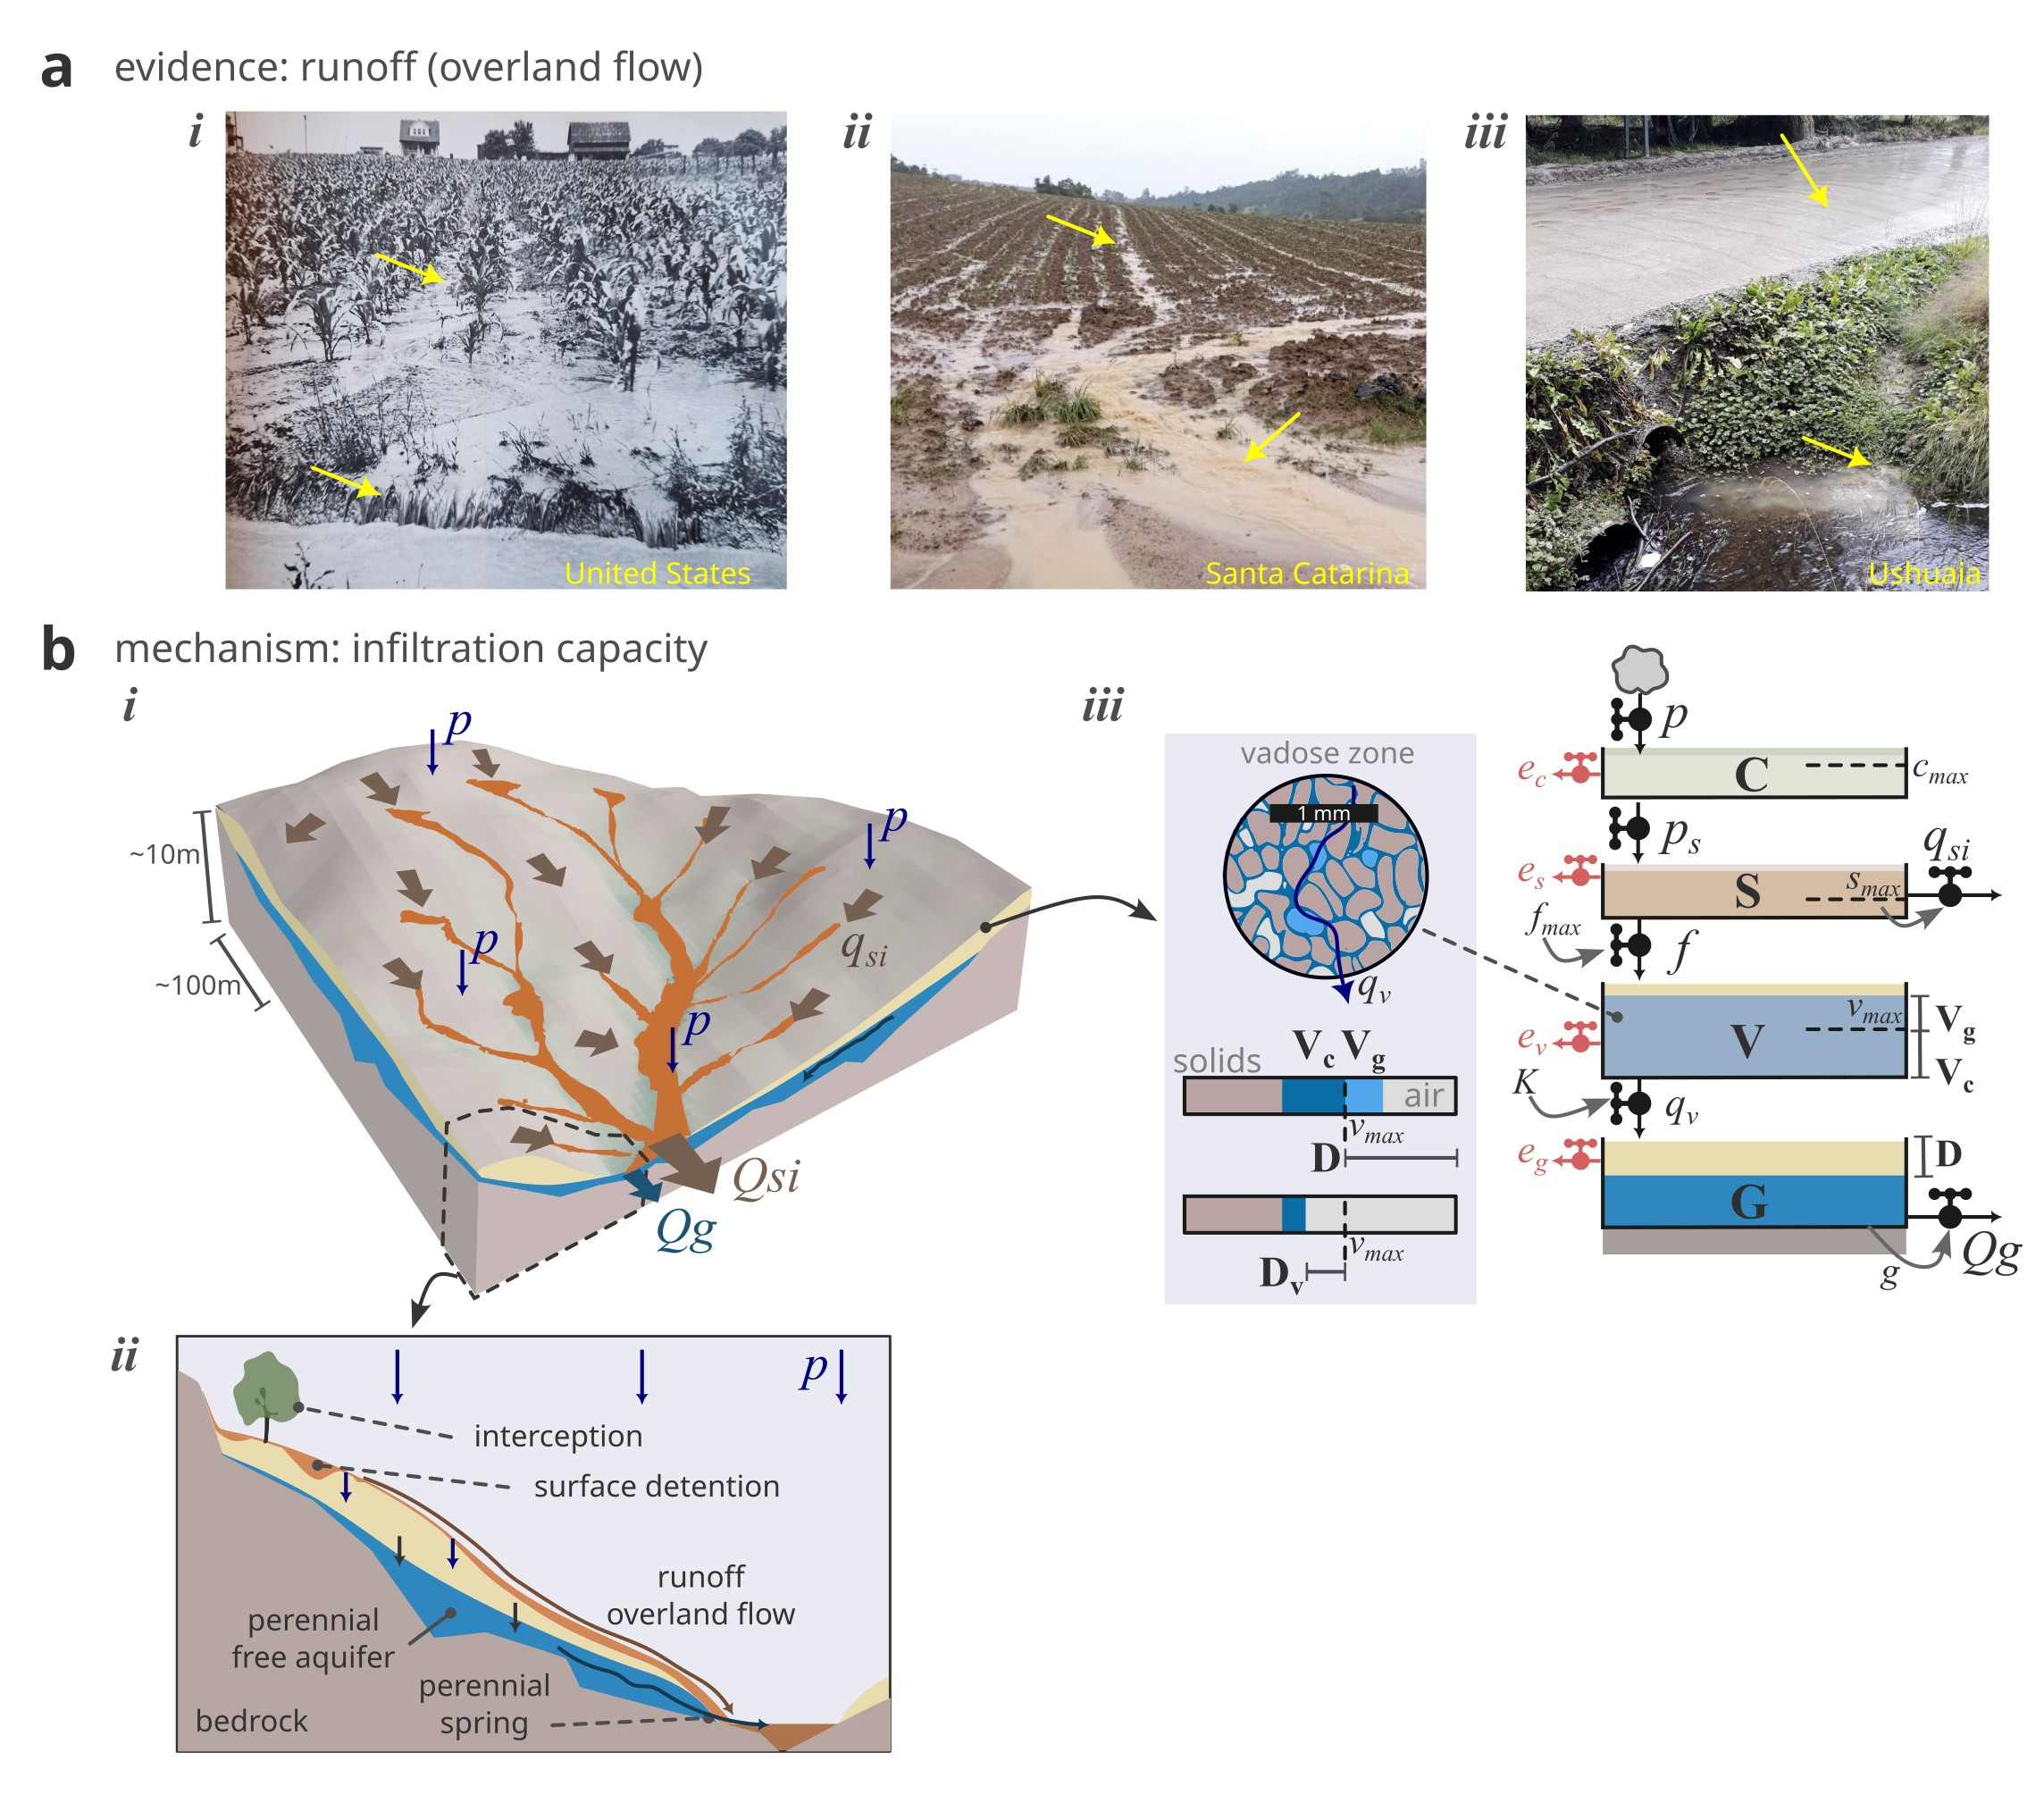
\includegraphics[width=0.98\linewidth]{figs/fig_horton_en.jpg}		
\caption[The Hortonian \gls{paradigma}]
{
\textbf{---\;The Hortonian \gls{paradigma}.} The Hortonian \gls{paradigma} explains the alternation between rises and recessions based on the concept of the soil’s \gls{infmax}.\;\textbf{a}\;---\;The motivating empirical evidence includes the surface runoff observed after rains when water fails to infiltrate: runoff in the United States reported by the \acrshort{scs} \cite{strahler1986} (detail \textrm{\textit{i}}); runoff in Santa Catarina reported by \texttt{EPAGRI} \cite{epagri2024} (detail \textrm{\textit{ii}}), and; rural road runoff in Ushuaia, authored by me (detail \textrm{\textit{iii}}).\;\textbf{b}\;---\;The \gls{sf-runoff} occurs generally in the basin (detail \textrm{\textit{i}}) from the moment when the rainfall flow exceeds the \gls{intercep-capacity} and the \gls{sfmax} (details \textrm{\textit{ii}} and \textrm{\textit{iii}}).
}
\label{fig:hydro:horton} 		
\end{figure}

\par In Section \ref{sec:systems:model} of the previous chapter, I organized a prototype of a hydrological \gls{model} aimed at illustrating and articulating how \gls{sys-dyn} can be employed in the modeling process. The obtained \gls{concept-model}, maintained in a minimalist condition, was constructed primarily based on the perception that a watershed exhibits \textbf{fast and slow responses} to rainfall events, thus producing the phenomenon of alternation between \textbf{rises} and \textbf{recessions} in rivers \cite{Hewlett1967}. This is a fundamental perception in \gls{hydrology}: when it rains, rivers become agitated, the water gets muddier, and levels rise (fast response); between rains, rivers calm down, the water becomes clearer, and levels fall (slow response); if too much time passes before it rains again, smaller streams begin to dry up (the \gls{system} tends to empty). With some empirical rigor, this phenomenon in any given watershed can be measured and reproduced in graphs with the aid of a rain gauge and a level stick. With a bit more empirical rigor, the perception of this phenomenon becomes sharper through field expeditions, observing the spatial and temporal dynamics of springs and puddles (where groundwater slowly surfaces) and the rapid runoff (caused by more intense rains).

\par In the context of zero-order basins, the dominant scientific \gls{teoria} today postulates that hydrological responses to rainfall events are the consequence of \textbf{multiple mechanisms of runoff generation}, both surface and subsurface, encompassing fast and slow responses, whether simultaneous or not, which will be described in the next section. These mechanisms were revealed and corroborated by successive experimental investigations in small basins, hillslopes with trenches, and soil plots during a scientific revolution in \gls{hydrology} that took place throughout the second half of the twentieth century. Before this revolution, however, the hegemonic scientific explanation for the fast and slow responses of hillslopes was primarily based on the hydrological \gls{teoria} of Robert Horton (1875-1945) \cite{Horton1933, Beven2004a}. Once published, the \gls{percept-model} described by Horton solidified as a true \gls{paradigma} in the following years and decades, marking the so-called \textbf{\gls{age_inf}} -- a long period of \gls{ciencia-normal} in which the \gls{comunidade-cientifica} developed research in both pure and applied fronts to articulate its implications \cite{Cook1946, Beven2021b}. Although ultimately surpassed by a more complex explanation, Horton’s \gls{teoria}, being scientific (i.e., falsifiable), greatly contributed to elevating \gls{hydrology} from its Empirical Era, focused on engineering applications, to being understood as a Geoscience, aimed at explaining natural phenomena.

\par The central idea of Horton’s \gls{percept-model} is established in the paper \textit{The role of infiltration in the hydrological cycle} (1933) \cite{Horton1933}, in which the soil is conceived as a \textit{separating surface} for rain: a portion of the rainwater infiltrates into the hillslopes, lodging in the soil matrix, while another portion runs off superficially as \textbf{runoff}, causing dramatic increases in river flow downstream (Figure \ref{fig:hydro:horton}\textbf{a}). Thus, \textbf{\gls{infiltration}} would be the key process for understanding the \gls{hydro_cicle} in its terrestrial phase:

\begin{adjustwidth}{100pt}{0pt}
\medskip
\small Infiltration divides rainfall into two parts, which thereafter pursue different courses through the hydrologic cycle. One part goes via overland flow and stream-channels to the sea as surface-runoff; the other goes initially into the soil and thence through ground-water flow again to the stream or else is returned to the air by evaporative processes. The soil therefore acts as a separating surface, and the author believes that various hydrologic problems are simplified by starting at this surface and pursuing the subsequent course of each part of the rainfall as so divided, separately. -- Robert Horton (1933, p. 446–447) \cite{Horton1933}. 
\medskip
\end{adjustwidth}

\par To articulate this \gls{percept-model}, Horton instantiates various flows, reservoirs, and important \gls{parameters} of the \gls{system} representing the \gls{zero-basin}. Figure \ref{fig:hydro:horton}\textbf{b} illustrates the modeled \gls{system} (the evapotranspiration flows in each reservoir are denoted by $E$). The primordial flow consists of \textbf{\gls{ground-rain}}, that is, the flow of rain that actually reaches the soil after the rain $p$ exceeds the \gls{intercep-capacity} in the \gls{canopy}. The soil, in turn, consists of a porous matrix of solid minerals that stores water in films maintained by the surface tension of its particles, thus forming the \textbf{\gls{unsat-zone}}. The accumulation of water in the films in this zone occurs up to a certain limit, which is the characteristic \textbf{\gls{fmc}} of the soil. This water in the \gls{unsat-zone}, which is trapped in the pores, is referred to as \textbf{\gls{water_capilar}}. In addition to the \gls{fmc}, the films of water on the particles, when mixed, create a relatively mobile mass of water, termed \textbf{\gls{water_gravit}}. This water then percolates vertically through the pores due to gravity, forming a \textbf{\gls{sat-zone}} above the impermeable layer, which is the solid rock foundation (i.e., this zone forms an unconfined aquifer). Horton refers to \textbf{\gls{qv}} as the vertical flow of water suspended in the \gls{unsat-zone} to the aquifer of the \gls{sat-zone}, a process that can eventually raise the groundwater level (thus increasing the hydraulic load in this porous \gls{system}). In this context, \textbf{\gls{dgrav}} represents the amount of \gls{water_gravit} in the \gls{unsat-zone} necessary to achieve complete soil saturation and, consequently, the emergence of the groundwater table at the surface. Here, the maximum flux of \gls{qv} is limited by the \textbf{\gls{cond-hyd}} of the soil: the closer the \gls{unsat-zone} is to saturation, the vertical percolation tends to be dominated by the hydraulic load, overcoming surface tension.

\par At this point, Horton introduces a crucial parameter in his \gls{percept-model}: the \textbf{\gls{infmax}}, that is, the maximum \gls{flux-max} of infiltration that the soil surface can offer at any given moment. It is important to highlight that this capacity is an attribute of the thin top layer of soil and, according to Horton, tends to be lower than the \gls{cond-hyd} of the soil matrix, functioning as a critical limiting factor in the \gls{system}. Thus, water from a \gls{ground-rain} with an intensity less than or equal to \gls{infmax} is completely absorbed by the soil matrix. On the other hand, when a \gls{ground-rain} has an intensity greater than \gls{infmax}, the water from the \textbf{\gls{ex-rain}} begins to fill the small surface depressions. If the \gls{ex-rain} persists long enough, the \textbf{\gls{sfmax}} is exceeded, and the process of \gls{sf-runoff} or \textbf{\gls{rie}} begins, where the rainwater flows through furrows and ravines downhill until it reaches the channels of the streams.

\par The \gls{infmax} depends on soil type, texture, and management practices, which implies variability in the response of different basins, even when subjected to identical rainfall events. In addition to spatial variability, Horton argues that the \gls{infmax} of the soil varies over time, dynamically oscillating between extremes of minimum and maximum capacity, in a \textbf{decay and restoration cycle} (Figure \ref{fig:hydro:horton2}\textbf{a}). In this cycle, the decay phase occurs during rainfall events due to the expansion of colloidal particles, clogging by fine particles, and compression caused by the impact of raindrops. On the other hand, the restoration phase occurs during dry periods as new cracks and pores open up due to the retraction of colloidal particles, thermal expansions, and the activity of soil fauna, such as insects and earthworms. With this conception, it is expected that a long rain, even of relatively low intensity, will eventually produce \gls{sf-runoff} if the ongoing decay leads the soil’s \gls{infmax} to a value \textit{below} the intensity of the \gls{ground-rain}. Furthermore, this concept introduces the effect of \textbf{\gls{amc}}, such as the difference in responses between the beginning and the end of a rainy season or during the onset of a cold front with persistent rains. In this case, if the restoration speed of the soil’s \gls{infmax} is relatively slow, subsequent rains, even if \textit{less} intense, tend to produce \textit{more} \gls{sf-runoff} than the initial rains. In other words, the behavior of the \gls{system} becomes highly non-linear.

\par With the \gls{teoria} regarding the role of infiltration in the \gls{hydro_cicle}, Horton then advances to definitively explain the phenomenon of rises observed in rivers, proposing a method for separating the hydrograph (Figure \ref{fig:hydro:horton2}\textbf{b}). To this end, he argues that total runoff consists of two separable flow components: (1) the groundwater flow, which is a slow response from the unconfined aquifer, and; (2) the surface runoff, which is a rapid response of runoff produced on the hillslopes. Both responses are controlled, in whole or in part, by the soil’s \gls{infmax}:

\begin{adjustwidth}{100pt}{0pt}
\medskip
\small In accordance with this theory, total runoff consists of two parts: (1) Suface-runoff, which is dependent on rainfall-amount, rain-intensity, and infiltration-capacity and is practically independent of evaporation-rate. (2) Ground-water runoff. This is dependent on (a) total infiltration and hence indirecty on the same factors which control surface-runoff and is also dependent on (b) vegetational activity and evaporation, which in part determine the water losses, and on (c) the complex interrelations between infiltration-capacity, field moisture-capacity, vegetational activity, and accretion to the water-table. -- Robert Horton (1933, p. 454) \cite{Horton1933}.
\medskip
\end{adjustwidth}

\noindent Assuming that the \gls{sat-zone}, the unconfined aquifer, functions as a \gls{linear-reserv}, the \textbf{\gls{deple-curve}} of the ground flow, or flow of discharge, consists of a typical \gls{curve-exp-dec} of the type $Q_{g} = Q_{g, o} e^{-t/g}$. This curve is a physical characteristic, and the \gls{g-coef} can be extracted from hydrographs during dry periods when water losses due to evapotranspiration are minimal (for example, in the colder months in temperate and subtropical climates). Once obtained, the \gls{deple-curve} can be horizontally shifted on the hydrograph, allowing for the separation of the surface component of river flow from the purely subsurface contribution. Thus, Horton proposes that there are four possible typologies of \gls{hydro-response} to rainfall events. The \textbf{Type 0} response occurs when the intensity of \gls{ground-rain} is less than \gls{infmax} and the total infiltrated water is below the \gls{fmd} (there is \textit{no} \gls{sf-runoff} and \textit{no} recharge). In this situation, even though it has rained, there is no detectable change in the river's \gls{deple-curve}. The \textbf{Type 1} response occurs when the intensity of \gls{ground-rain} is less than \gls{infmax}, but the total infiltrated water is greater than \gls{fmd} (there is \textit{no} \gls{sf-runoff} but \textit{there is} \gls{qv} from the aquifer). In this case, the \gls{deple-curve} is shifted, depending on how much the \gls{qv} exceeds (or falls short of) the discharge flow, potentially producing a (relatively slow) pulse in the river flow purely from the increase in hydraulic load in the aquifer \gls{system}. The \textbf{Type 2} response occurs when the intensity of \gls{ground-rain} exceeds \gls{infmax} and the total infiltrated is very low, below \gls{fmd} (there is \textit{sf-runoff} but \textit{no} \gls{qv} from the aquifer). This type of response consists of a rapid pulse of surface runoff water superimposed on the \gls{deple-curve} that was developing before the event. Finally, the \textbf{Type 3} response happens when both the fast and slow responses occur simultaneously: both \gls{sf-runoff} and \gls{qv} from the aquifer manifest as overlapping pulses. These four typologies illustrate the complexity that emerges from Horton’s \gls{percept-model}, providing significant leeway for explanations of rises that vary according to the characteristics of the surface, soil, subsurface, rainfall, and antecedent moisture conditions.

% figure
\begin{figure}[t!] 
\centering				
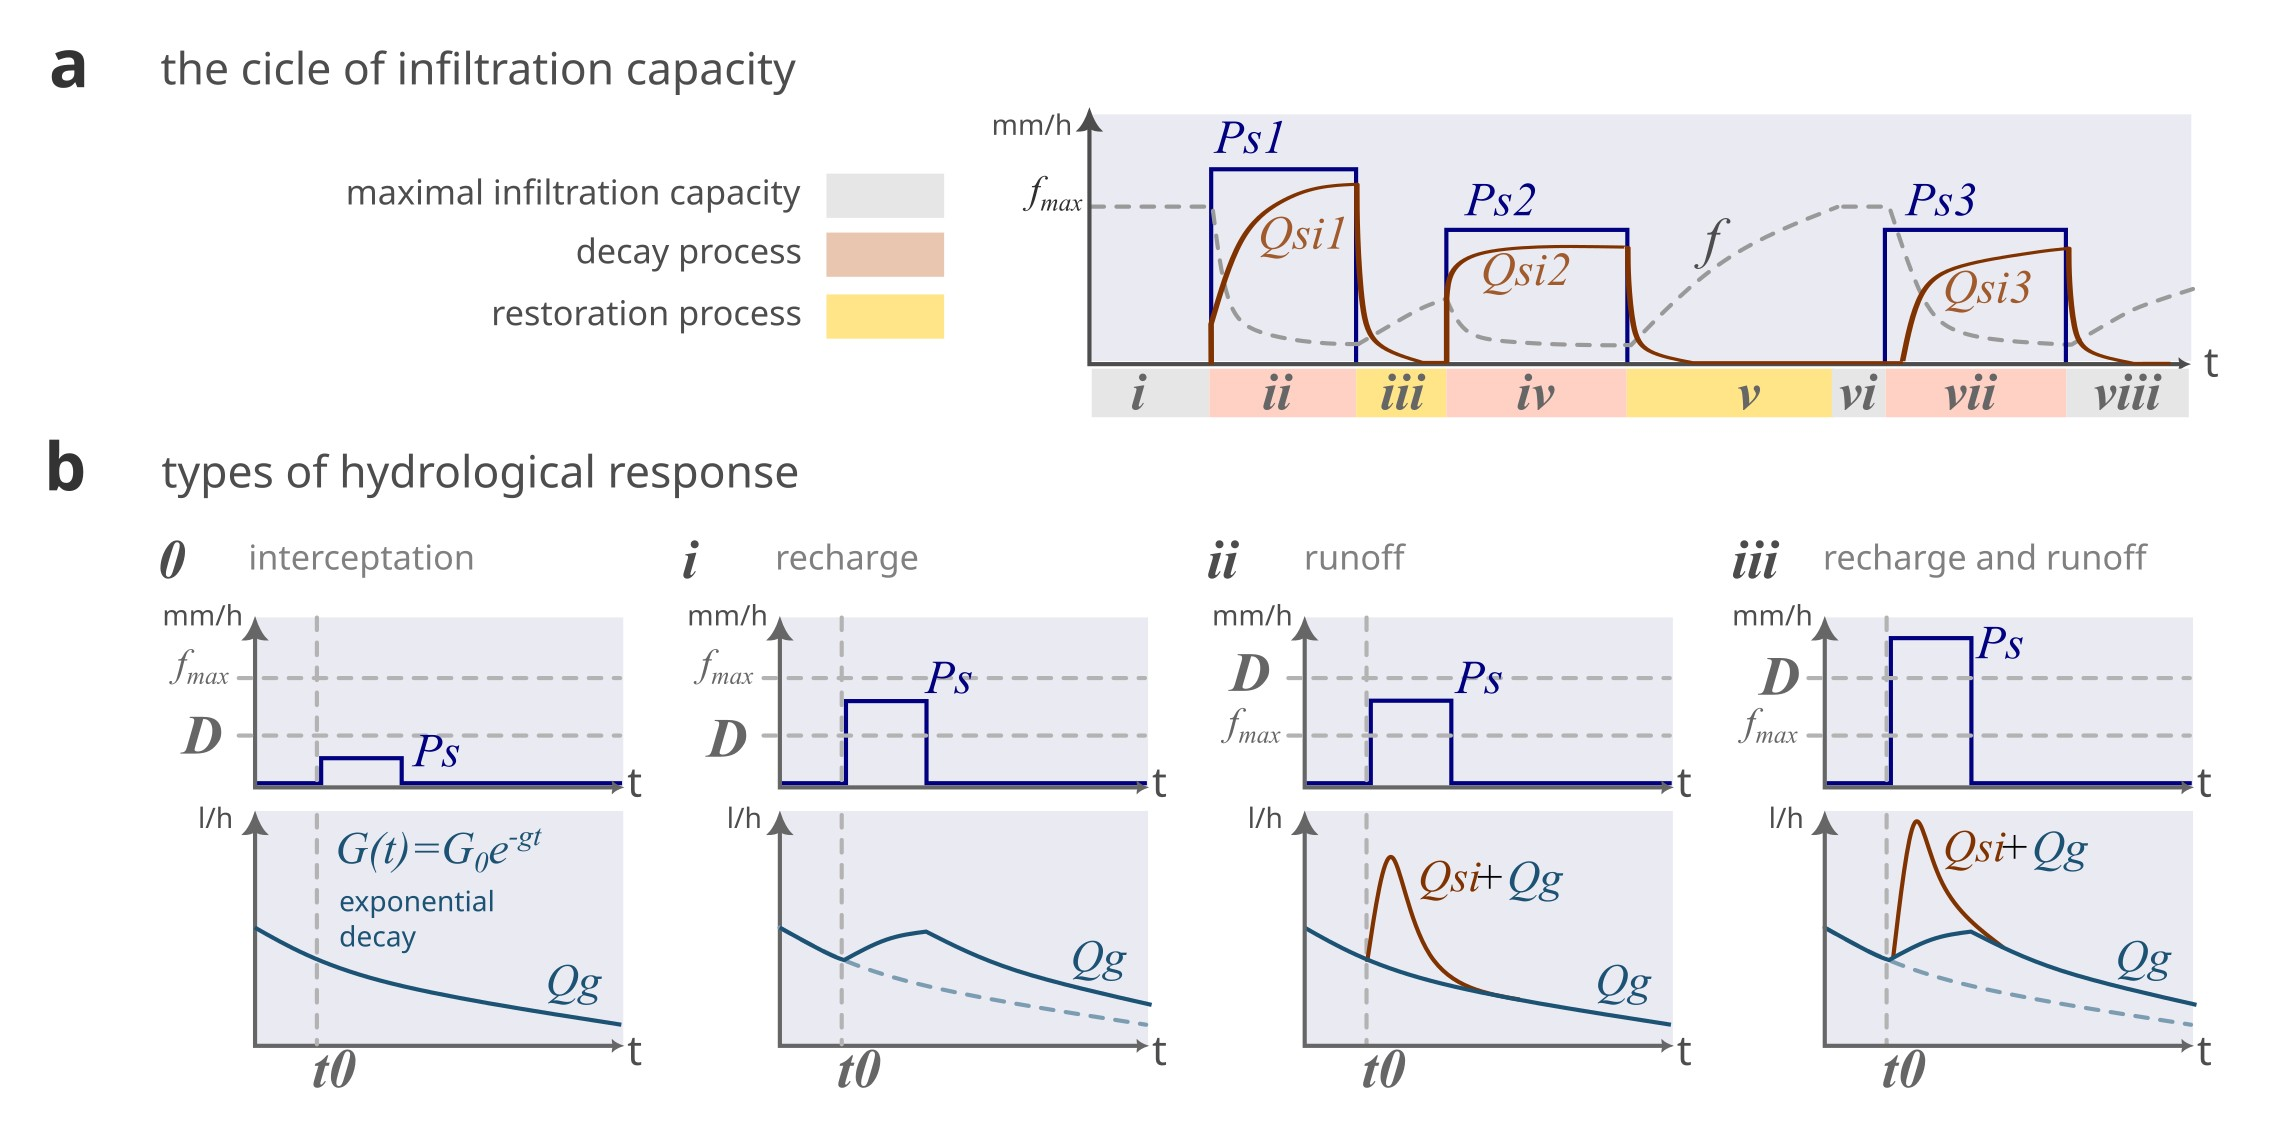
\includegraphics[width=0.98\linewidth]{figs/fig_horton2_en.jpg}		
\caption[Implications of the Hortonian \gls{model}]
{\textbf{---\;Implications of the Hortonian \gls{model}.}
    \textbf{a}\;---\;The capacity for \gls{infiltration} goes through cycles of decay and restoration, generating non-linearities, such as the fact that identical rains ($P_{g,2}$ and $P_{g,3}$) produce different fast responses ($Q_{s,2}$ and $Q_{s,3}$) (details \textrm{\textit{iv}} and \textrm{\textit{vii}}).\;\textbf{b}\;---\;It is also possible to deduce different typologies of \gls{hydro-response}: Type 0, when rain produces neither recharge nor runoff (no response, detail \textrm{\textit{0}}); Type 1, when rain produces only recharge (slow response, detail \textrm{\textit{i}}); Type 2, when rain produces only runoff (fast response, detail \textrm{\textit{ii}}), and; Type 3, when rain produces both a slow and a fast response (detail \textrm{\textit{iii}}).
}
\label{fig:hydro:horton2} 		
\end{figure}

\par In light of this \gls{percept-model}, various conceptual models have been developed through physical approaches (when physical principles are applied \textit{a priori}) and empirical approaches (when equations are fitted to data \textit{a posteriori}) \cite{mishra2003}. In the realm of the physical approach, notable advancements include those by Philip (1957) \cite{philip1957}, who laid the foundations for a mathematically formal \gls{teoria} of infiltration as a special case of the Darcy-Richards equation, that is, the movement of water in an unsaturated porous medium. On the empirical side, Robert Horton himself maintained an applied research line, proposing a \gls{concept-model} of exponential decay for the soil’s \gls{infmax} \cite{Horton1939}. Consequently, the production of experimentally standardized infiltration curves enabled a more sophisticated technique for estimating total \gls{sf-runoff}, in contrast to the rational method, which is based on a simple runoff coefficient \cite{Cook1946}. Another empirically influential method produced in this context was the \textbf{\gls{cn_method}}, developed by the \acrfull{scs} in 1954 and presented as a technical guideline in the following decades. According to Rallison \& Miller (1981) \cite{Rallison1981}, the \acrshort{cn} method from the \acrshort{scs} emerged from the results of experimental research in small basins, but was primarily motivated by the passage of environmental protection legislation in the United States. It is noted that Horton was a consultant for the \acrshort{scs}, but his infiltration curve method did not gain much traction, yielding to the aggregated approach of Mockus (1949) \cite{mockus1949}, which evaluates the relationship between total rainfall and runoff for individual events. Justified by this evidence, the equation of the \acrshort{cn} method seeks to express the supposed \textit{transition} from a \textit{non-linear} response (when infiltration and surface retention dominate the surface water balance) to a \textit{linear} response (when the intensity of \gls{ground-rain} exceeds \gls{infmax} and surface retention). The CN parameter, in this sense, calibrates the effect of non-linearity for different types of soil, land covers, management practices, and antecedent moisture conditions. Rallison \& Miller point out that the choice of this approach by the \acrshort{scs} had a strong convenience bias, as the data used were readily available on a national scale (in the United States). Nevertheless, the essence of the \acrshort{cn} method reproduces Horton’s \gls{percept-model}, as \gls{sf-runoff} is regarded as the only rapid response of the watershed and is determined by the estimate of \gls{ex-rain}.

\section{The age of differentiation}

\begin{figure}[t!] 
\centering				
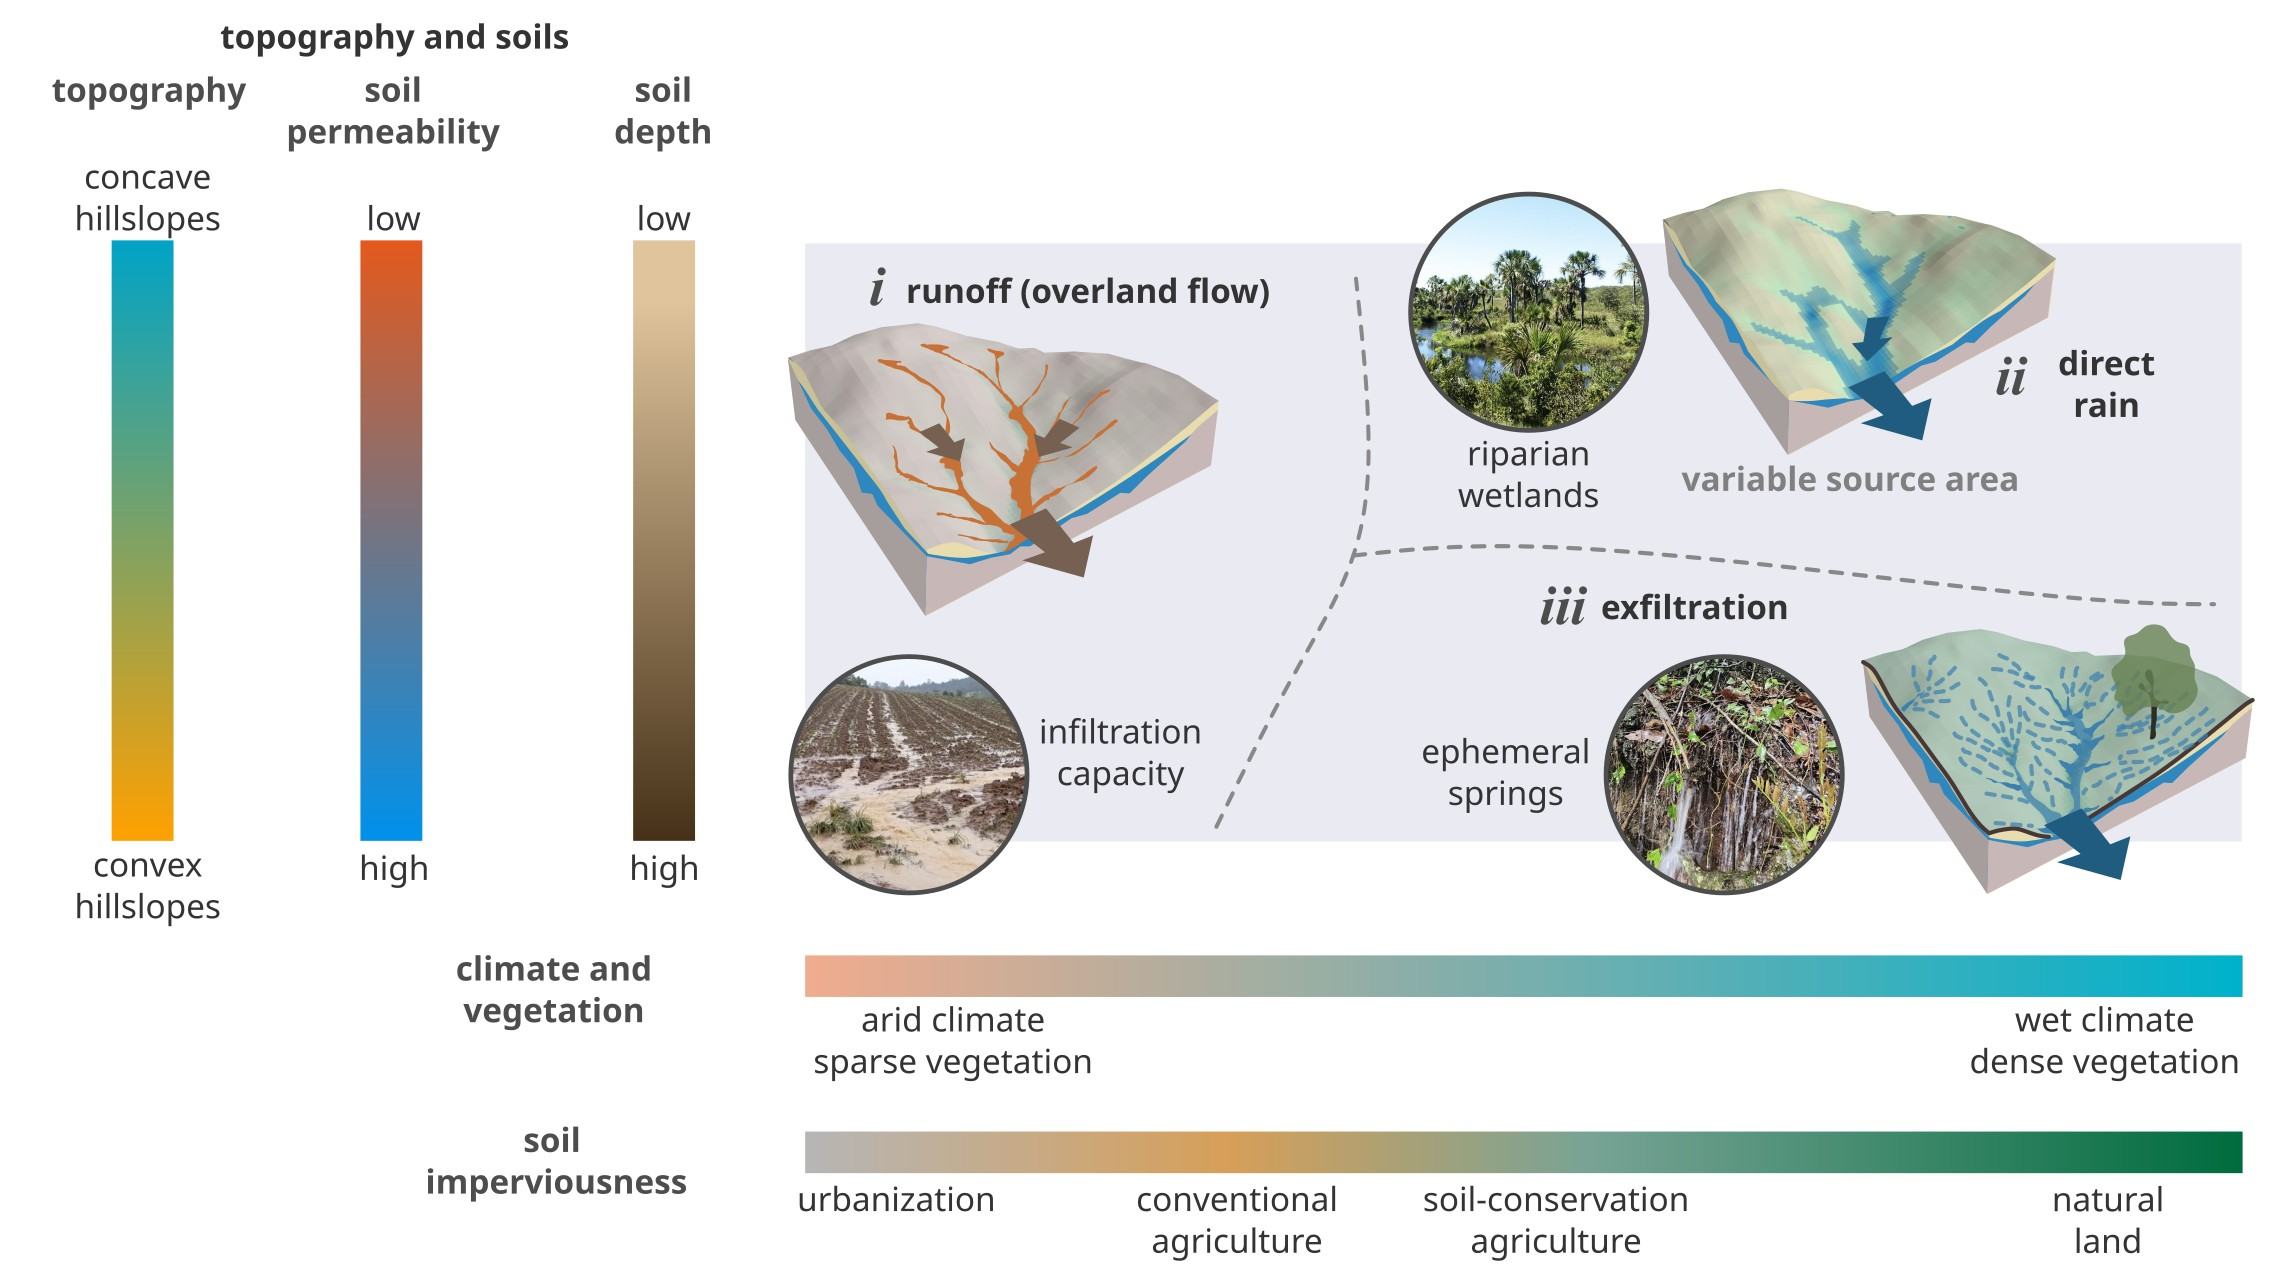
\includegraphics[width=0.98\linewidth]{figs/fig_processes_en.jpg}		
\caption[Differentiation of rapid response mechanisms.]
{\textbf{---\;Differentiation of rapid response mechanisms.}
    Schematic view proposed by Thomas Dunne (1983) \cite{Dunne1983} on the new \gls{paradigma} of rapid response mechanisms in zero-order basins. Runoff, considered the only mechanism in the Hortonian \gls{paradigma}, has been reserved for special conditions in arid climates or anthropized environments, such as farms or cities, where the soil’s infiltration capacity is very low (detail \textrm{\textit{i}}). At least two new mechanisms are differentiated: rapid responses due to saturation excess, or direct rain on \gls{sat_areas} (detail \textrm{\textit{ii}}), and; rapid responses due to exfiltration in \gls{nasc_efemeras}, dominant in deeper, structured soils with macropores (detail \textrm{\textit{iii}}).
}
\label{fig:hydro:diff} 		
\end{figure}

\par In Section \ref{sec:epis:kuhn}, I highlighted that, according to Thomas Kuhn, the success of a scientific \gls{teoria} is primarily associated with its \textit{competitiveness} in relation to other ideas circulating within the \gls{comunidade-cientifica}. Thus, a \gls{teoria} tends to establish itself as the hegemonic \gls{paradigma} when it efficiently explains known phenomena and opens promising avenues for investigation for new generations of researchers. In the absence of structured competing theories in this sense, Horton’s \gls{percept-model} for explaining rapid and slow hydrological responses provided these two attributes to a \gls{comunidade-cientifica} strongly marked by \gls{bias-engineer} and \gls{bias-fluvial}. These two characteristics have a shielding effect on perceptions that are technically irrelevant for solving typical downstream problems, as they do not require details about what happens in zero-order basins. Ironically, this was precisely the objective of the \acrshort{scs} -- to protect the soil on the hillslopes. The Hortonian \gls{model}, whether partially or completely incorrect, did not prevent good estimates of design flows for bridges, dams, and water balance in large basins, among others. After all, the equifinality of systems allows similar behaviors to manifest from distinct mechanics (until the day everyone is surprised). In strictly technical terms, to some extent, the development of the \acrshort{cn} method by the \acrshort{scs} \textit{perpetuated} the ideas of the \gls{age_inf}, being generally the basic method required or accepted by technical guidelines in engineering projects and the main module for generating runoff in various distributed hydrological models in software such as \texttt{SWAT} and \texttt{SWMM}.

\par Although the \gls{paradigma} of infiltration may have consolidated simply due to a lack of competitors, its crisis has been present since its formation in the 1930s and 1940s. For example, the rainfall intensity and soil \gls{infmax} data measured by Horton’s own laboratory suggest that it is highly \textit{unlikely} he observed widespread \gls{sf-runoff} in his experimental basin at La Grange Brook (14.4 ha, New York) \cite{Beven2004c}. The laboratory data, evaluated by Keith Beven, indicate that the soil in the main covers of the basin (fields and orchards) exhibited a relatively high \gls{infmax} compared to the recorded rains. In fact, the reconciliation between Horton’s \gls{infmax} measurements of the soil \textit{in situ}, the \textbf{field value}, and estimates at the basin scale, the \textbf{effective value}, possibly never made much sense with each other, requiring numerous \gls{aux-hyp} and \gls{neglig-premis} (the \textbf{scale problem}, which we will address later). This was made clear in Betson's (1964) article \cite{Betson1964}, which achieved excellent fittings of a \gls{concept-model} to observed data only after \textit{relaxing} the Hortonian \gls{model}, implying a \textbf{partial contribution area} concept of surface runoff. From a rationalist perspective, Betson attempted to \say{save} Horton’s \gls{teoria} by admitting \textit{ad hoc} modifications to avoid its refutation. Even though statistically well-fitted, the results hinted that a small and relatively constant fraction of the basins in the Tennessee River valley produced \gls{sf-runoff} (basins ranging from 500 ha to 8.4 km², North Carolina).

\par However, it was throughout the 1960s that the \gls{age_inf} faced its ultimate crisis in the scientific realm. Not coincidentally, this period witnessed the \textbf{International Hydrological Decade} (1965-1974), a United Nations (\texttt{UNESCO}) program developed to promote research in \gls{hydrology}. The revolution in perceptions within the \gls{comunidade-cientifica} occurred after a profusion of empirical evidence accumulated in the literature, reporting the observation of new mechanisms of \gls{hydro-response} from hillslopes, which will be described in the following sections. At least three new rapid response mechanisms (or potentially rapid) can be summarized beyond those posited by Horton: (1) \textbf{\gls{subsur_flow}}, (2) \textbf{\gls{rse}}, and (3) \textbf{\gls{trans_flow}}. The first two refer to new rainwater contributing to rises. The last consists of old water stored underground, which also contributes to the rapid response (with surprisingly high prevalence rates). The nomenclature surrounding these mechanisms is somewhat confusing in the literature even today, perhaps due to the fact that water lacks a visible label, complicating differentiation out of context (for example, water emergence in springs can represent either a slow or fast response). In contrast to the Hortonian \gls{model}, these rapid responses include surface and subsurface pathways controlled by other parts of the \gls{system} beyond the topsoil, such as \textbf{\gls{macropor}} (preferential lateral and vertical pathways in the soil) and topography (dynamic patterns of soil saturation). Essentially, empirical evidence in the second half of the twentieth century irreversibly exposed the complexity of processes in zero-order basins.

\par A landmark for the beginning of the end of the \gls{age_inf} was Mike Kirkby's (1969) article \cite{Kirkby1969}, which reviewed results from various experimental studies and presented a new way to understand and name hydrological processes in zero-order basins. At this point, Kirkby (1969) definitively marks the importance of rapid responses of water moving through the soil via a network of macropores (subsurface runoff). After more than a decade of accumulating new empirical evidence, a landmark for the rise of the new \gls{paradigma} was Thomas Dunne's (1983) article \cite{Dunne1983}, which definitively organized a new schematic view of rapid hydrological responses, illustrated in Figure \ref{fig:hydro:diff}, proposing a promising new research program in both pure and applied fronts. Dunne (1983) makes clear the idea that different climates, scales, and landscapes favor the \textit{dominance} of one mechanism over another, even though they may occur simultaneously or alternate seasonally. For example, in semi-arid climates, factors such as long dry periods and the formation of soil crusts favor Horton’s mechanism—the \gls{infmax} tends to be insufficient, and there are often no saturated areas in valley bottoms at the end of the dry season. In contrast, in humid tropical climates, the formation of deep soils or excess water during the rainy season may favor either mechanism. Ultimately, this revolution produced new understandings of the complex relationships between these mechanisms, as demonstrated by Jeffrey McDonnell (1990) \cite{mcdonnell1990} in the case of the MaiMai Experimental Basin (New Zealand). However, McDonnell (2013) \cite{Mcdonnell2013} also critiques the entrenched \gls{paradigma}: the hegemonic research program primarily focuses on \textit{differentiating} the multiple hydrological responses, reaffirming the idea of complexity and uniqueness of each environment. While this attitude may continue \textit{ad infinitum}, he argues that the true objective of hydrological science might be to produce \textit{generalizations}, theories that are \textit{unifying}. In this spirit, the prevailing hydrological \gls{paradigma} might deserve the title of \textbf{\gls{age_diff}}.

\subsection{The function of macropores}

% figure
\begin{figure}[t!] 
\centering				
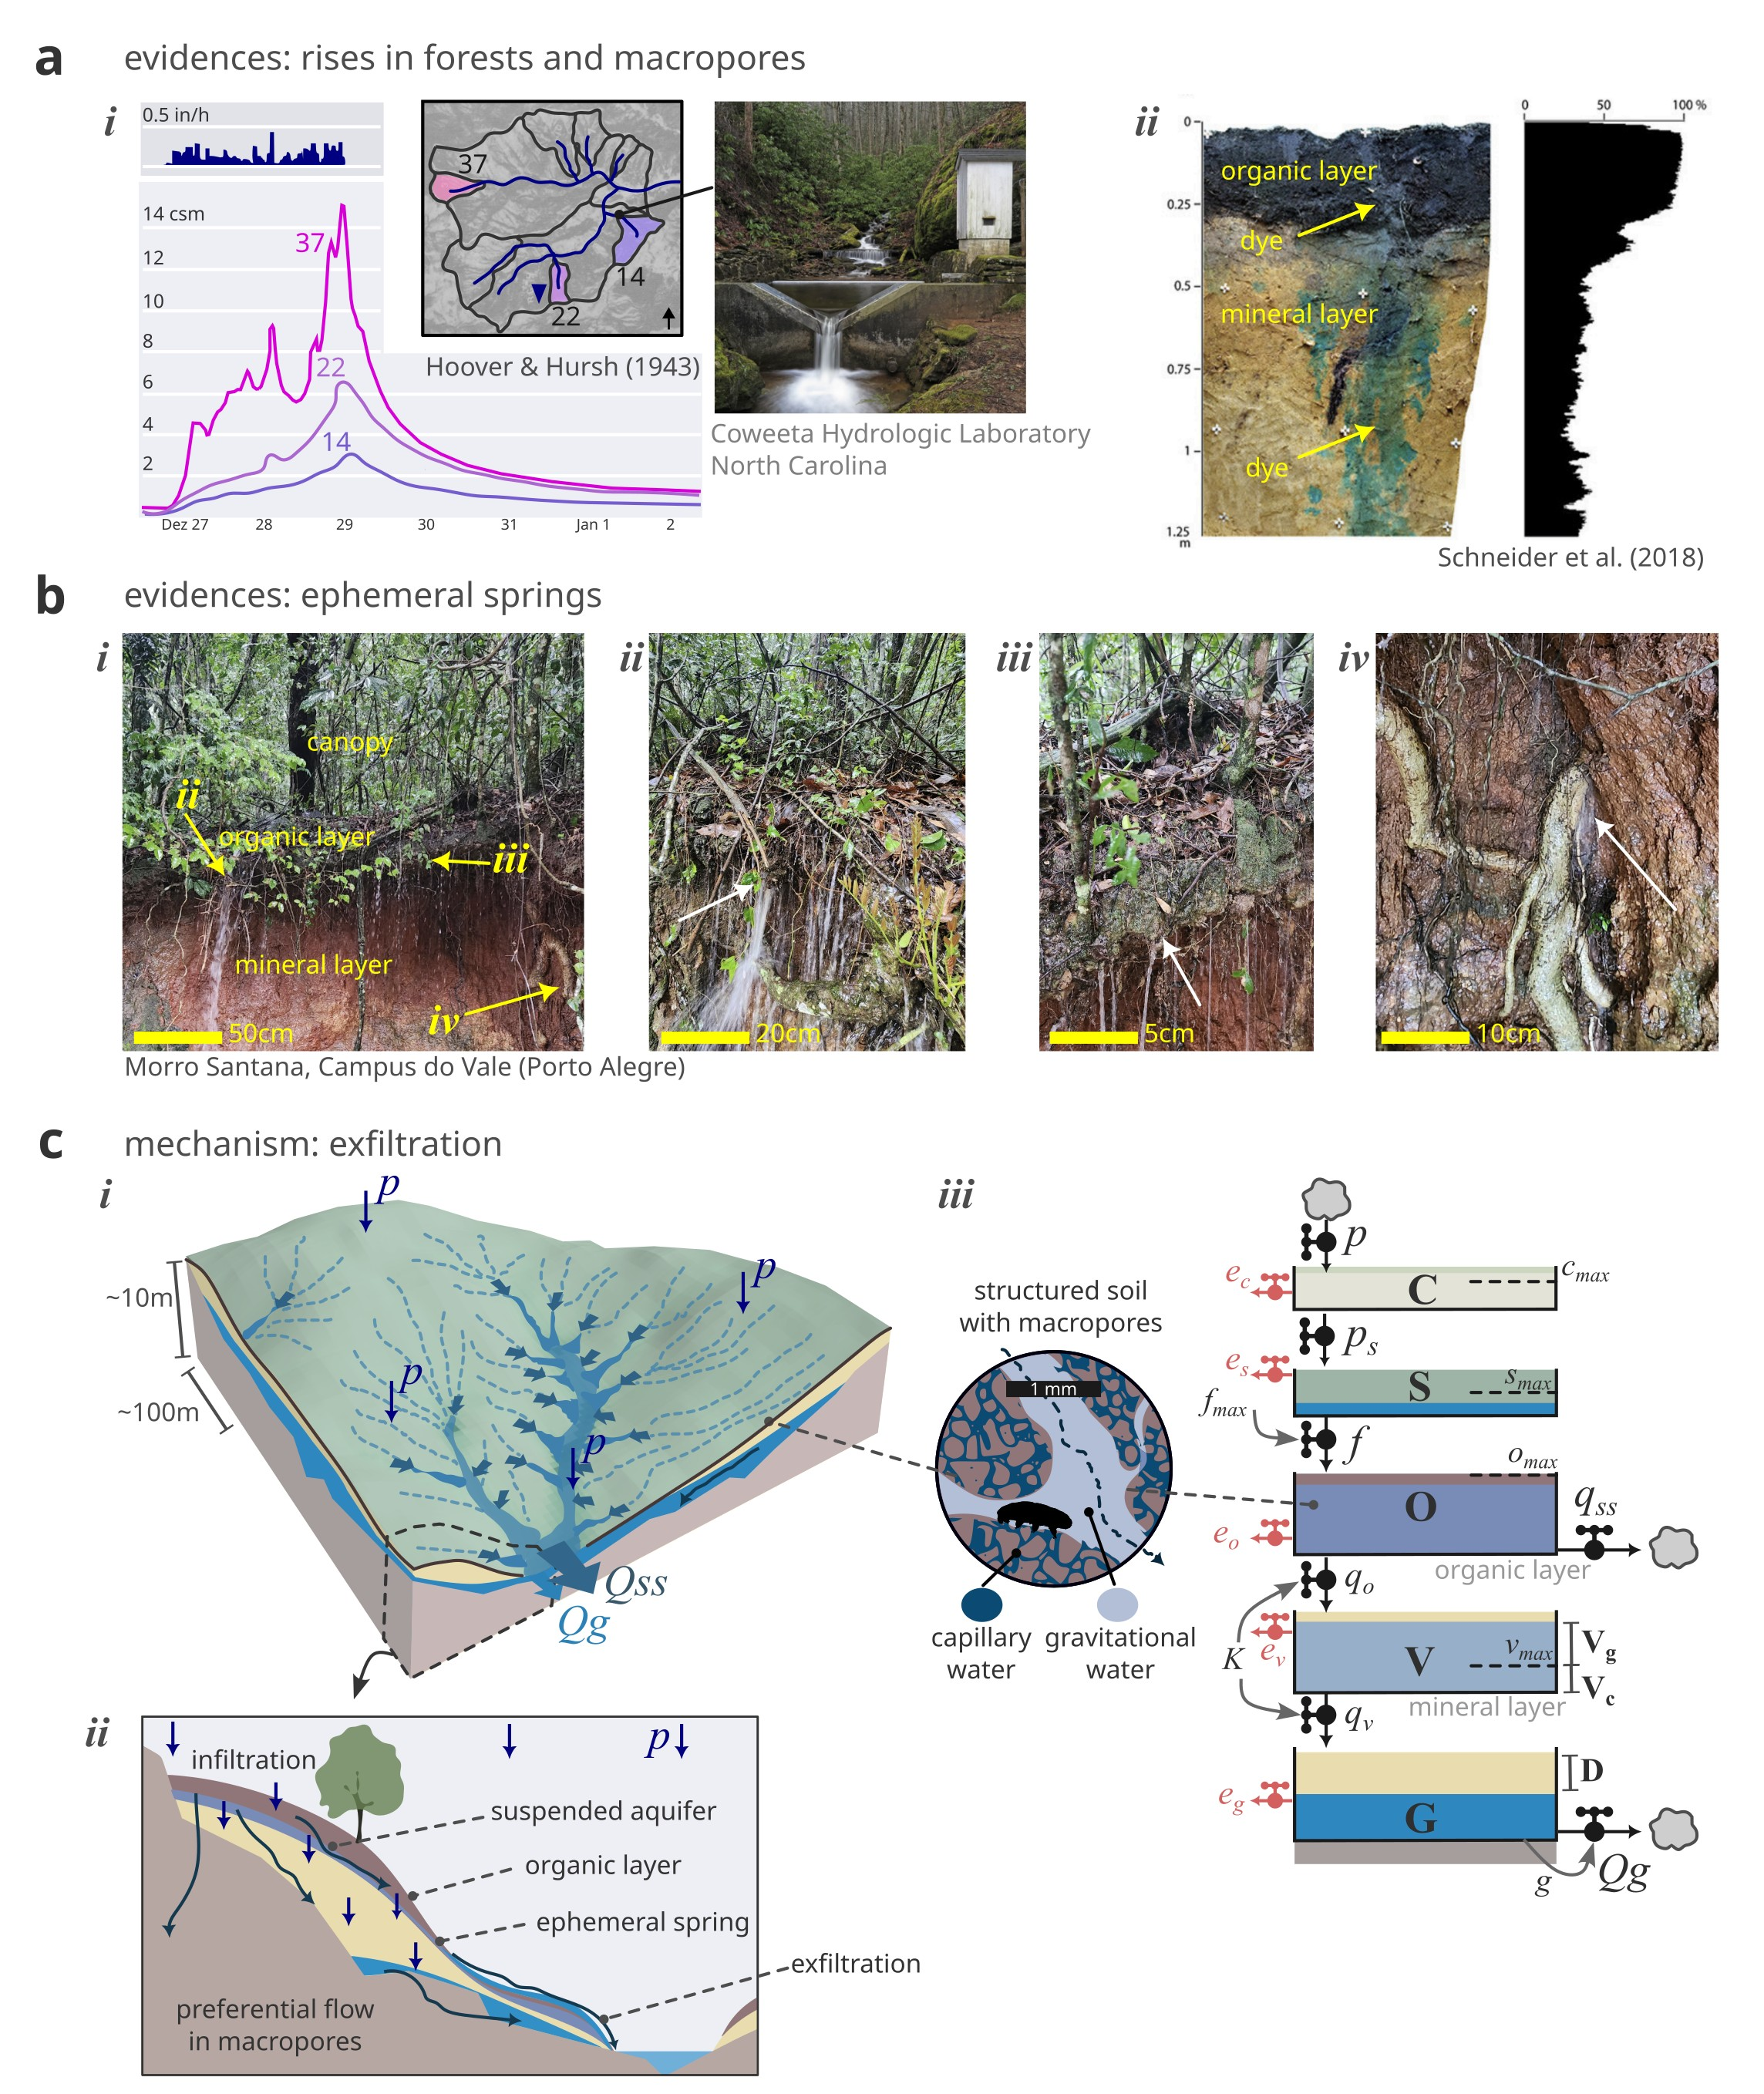
\includegraphics[width=0.98\linewidth]{figs/fig_macropores_en.jpg}		
\caption[Rapid exfiltration through macropores]
{\textbf{---\;Rapid exfiltration through macropores.}
    Macropores and preferential subsurface pathways produce rapid \gls{subsur_flow} responses, especially in forests.\;\textbf{a}\;---\;Evidence: rises without runoff in basins at the Coweeta Experimental Forest (North Carolina, United States) reported by Hoover \& Hursh (1943) \cite{Hoover1943} (detail \textrm{\textit{i}}), and; the distribution of macropores in the soil profile highlighted by dyes, reported by Schneider et \text{al.} (2018) \cite{Schneider2018} (detail \textrm{\textit{i}}).\;\textbf{b}\;---\;Evidence: \gls{nasc_efemeras} observed on June 16, 2023, at a road cut on the Vale Campus of the Federal University of Rio Grande do Sul (Morro Santana, Porto Alegre). Despite the extraordinary rain on that day (141.7 mm in 24 hours), no runoff was observed in the forest soil. \textrm{\textit{i}} -- profile of the bank; \textrm{\textit{ii}} -- preferential flow; \textrm{\textit{iii}} -- flow at the interface between horizons; \textrm{\textit{iv}} -- turbulent flow in a fracture in granite, created by a root.\;\textbf{c}\;---\;Systematization of the \gls{nasc_efemeras} mechanisms: rainwater infiltrates rapidly, creating a suspended aquifer at the transition between the organic and mineral horizons. This suspended aquifer emerges at various points in the basin, facilitated by macropores and preferential subsurface pathways, creating \gls{nasc_efemeras} during and shortly after rainfall. Source of the photograph in \textbf{a}: https://www.be-roberts.com/se/cwta/cwta1.htm .
}
\label{fig:hydro:macro} 		
\end{figure}

\par In the late 1930s and early 1940s, the scientific literature already recognized the weaknesses of Horton’s \gls{model}, asserting that the rapid response of small basins should include one or more \textit{subsurface} mechanisms. Snyder (1939) \cite{Snyder1939}, for example, suggests using the term direct runoff to denote the rainwater that contributes to the river flood \textit{without ever having moved through the soil}. In this context, Barnes (1939) \cite{Barnes1939} divides the components of river flow into \textit{three} (rather than \textit{two}): (1) surface runoff; (2) storm seepage; and (3) base flow. By \say{storm seepage}, Barnes referred to a rapid subsurface flow of rainwater that moves \textit{laterally} through the \gls{unsat-zone}, feeding the stream channels at a much faster rate than expected from the \gls{g-coef}:

\begin{adjustwidth}{100pt}{0pt}
\medskip
\small This consists of water which has penetrated only the upper soil-layers during a rainstorm or a thaw and has filtered more or less horizontally through the soil to discharge into the stream-system by seepage. It was observed by the writer in 1936 while analyzing discharge records of Zumbro River in Minnesota and called by him \say{secondary base-flow}. -- Bertram Barnes (1939, p. 721) \cite{Barnes1939}.
\medskip
\end{adjustwidth}

\noindent Thus, a distinction is made between \textbf{\gls{nasc_perenes}}, fed by the flow of true groundwater (unconfined aquifer), and \textbf{\gls{nasc_efemeras}}, fed by the subsurface flow of rainwater (suspended aquifer). This response mechanism was greatly reinforced by studies conducted by Charles Hursh at the Coweeta Experimental Forest (North Carolina, United States), with results reported for various forested basins ranging in size from 16 to 760 hectares \cite{Hoover1943, Hursh1944}, generating the \gls{model} illustrated in the details of Figure \ref{fig:hydro:macro}\textbf{c}. For example, Hursh \& Brater (1941) \cite{Hursh1941} claim that \gls{sf-runoff} was never observed on the hillslopes of one of the monitored basins, despite the rapid responses observed in river flow:

\begin{adjustwidth}{100pt}{0pt}
\medskip
\small Surface storm-runoff as overland-flow has not been observed on this drainage-area; nevertheless, characteristic flood-hydrographs are produced by heavy rains. -- Hursh \& Brater (1941, p. 863) \cite{Hursh1941}.
\medskip
\end{adjustwidth}

\noindent This claim, followed by data in subsequent studies (see Figure \ref{fig:hydro:macro}\textbf{a}, in detail \textit{i}), inevitably introduces a \textit{counterexample} to the \gls{teoria} of \gls{infmax}. After all, if there is no \gls{sf-runoff}, the only available response in Horton’s \gls{percept-model} is the \textit{slow} response caused by the \gls{qv} from the aquifer, which is responsible for the \gls{deple-curve}. Among other mechanisms at work in the basin, detailed later, the authors point to the existence of \textit{rapid subsurface responses} that include both water flow in highly permeable soil layers (unsaturated flow) and the formation of temporary suspended aquifers (saturated flow), which develop in different parts of the landscape during rainfall. In this regard, Hursh \& Fletcher (1942) \cite{Hursh1942} emphasize the importance of soil \gls{macropor}. Especially in forests, this property would help explain the dominance of preferential subsurface flows, significantly increasing the soil’s \gls{water_gravit}, in contrast to \gls{water_capilar}:

\begin{adjustwidth}{100pt}{0pt}
\medskip
\small The exact nature of this macro-pore space occurring in different horizons of the soil profile has yet to be described. It includes all large underground channels formed from decayed roots, fractured rock, insect and animal burrows, and larger spaces that may exist. It also includes macro-pore spaces formed through the complex structural patterns created by the aggregation of soil particles in the presence of organic materials. In the upper horizons of natural soils these biological openings and structural patterns built up from lattice-like aggregates are far more important in determining noncapillary porosity than the single grain soil particle size. Root channels and animal burrows are of particular significance in the detention storage and draining of gravitational water. A single earthworm burrow may be far more important in draining through a block of heavy soil than the entire cross sectional area of the pore space. In like manner, it is conceivable that a few continuous void spaces may give rise to rapid discharge of groundwater through a soil profile which, when viewed as a uniformly pervious medium, would be expected to transmit water slowly. -- Hursh \& Fletcher (1942, p. 485) \cite{Hursh1942}.
\medskip
\end{adjustwidth}

\par Unlike recent studies with dyes, which clearly demonstrate the existence of macropores (as shown in detail \textit{ii} of Figure \ref{fig:hydro:macro}\textbf{a}, with recent results from Schneider et \text{al.} (2018) \cite{Schneider2018}), the authors from Coweeta presented no evidence beyond observations of aggregated processes, such as rain, flow, and well levels. This research gap was permanently addressed in the 1960s when a new wave of studies provided more detailed quantitative results obtained through a more experimental approach than observational. Still in the context of the Coweeta Experimental Forest, Hewlett and Hibbert (1963) \cite{Hewlett1963} used a lysimeter to demonstrate the critical role of water flow in the \gls{unsat-zone} in sustaining base flow in streams. Whipkey (1965) \cite{Whipkey1965} detailed lateral flows in the soil profile of a hillslope in Ohio (USA). The hillslope was monitored by a trench at its base, demonstrating the dynamics of \gls{subsur_flow}, especially in the upper organic layers, where high \gls{cond-hyd} was measured due to the presence of macropores. Here, the function of \textbf{\gls{perm_trans}} between the soil horizons appears, especially between the \gls{o-horizon} (upper) and the mineral horizon (lower). This discontinuity generates a loss of hydraulic head that results in \textit{lateral} flow in the \gls{unsat-zone}. I personally observed this process during a severe storm on June 16, 2023, at the Vale Campus of the Federal University of Rio Grande do Sul, at the base of Morro Santana, Porto Alegre (see details in Figure \ref{fig:hydro:macro}\textbf{b}). According to the \texttt{INMET} Station \texttt{83967}, June 16, 2023, recorded 141.7 mm of rain, which is above the monthly average for that month (around 130 mm). Despite such extreme rain and streams practically overflowing, I did not observe surface runoff in the forested areas of the campus, except where the terrain's channel forced the emergence of the suspended aquifer (i.e., through the expansion of riparian wet areas).

\par Other trench studies reaching similar conclusions to Whipkey's (1965) in the United States include: Ragan (1968) in Vermont \cite{Ragan1968}; Beasley (1976) in Mississippi \cite{Beasley1976}, and; Harr (1977) in Oregon \cite{Harr1977}. In the latter case, it was reported that \gls{subsur_flow} was 6 to 9 times greater in the upper soil layers than in the lower layers, corroborating the function of \gls{macropor}. In the same study, the authors report that \gls{subsur_flow} was responsible for about 97\% of the rapid response during rises. This was consistent with earlier results from Patric and Swanston (1968) \cite{patric1968}, who cut down all the trees on a slope in Alaska and applied sprinkler irrigation. They observed no \gls{sf-runoff} -- the applied water traveled through preferential subsurface pathways, emerging rapidly at the base of the slope. In the British Isles, Weyman (1970) \cite{weyman1970} reported that unsaturated subsurface runoff constitutes the main rapid response in an experimental basin, while Jones (1971) \cite{Jones1971} noted that the widespread occurrence of the phenomenon known as \textit{piping} -- the formation of natural tunnels in the soil profile -- contributes to high velocities in subsurface response. Consolidating this new generation of field research, results from the MaiMai experimental basin (New Zealand) established a new experimental research program, combining water balance, trenches, and the novelty of chemical tracers, dyes, and isotopes. In the case of MaiMai, Mosley (1979) \cite{Mosley1979} reaffirms (almost forty years after Hursh) the crucial role of \gls{macropor} and natural tunnels in \gls{subsur_flow} while addressing some theoretical objections:

\begin{adjustwidth}{100pt}{0pt}
\medskip
\small Freeze [1972, p. 1282] considerou que um valor limiar de condutividade hidráulica saturada da ordem de 0,002 cm/s é necessário para que a \gls{subsur_flow} seja significativa, mas em um solo que contém canais de raízes, túneis e zonas de afloramento, a condutividade hidráulica saturada não é um fator limitante. O fluxo de corante traçador através de macroporos no solo foi observado a taxas até 3 ordens de magnitude maiores, e a resposta sensível e rápida da \gls{subsur_flow} às variações na precipitação sugere que o fluxo por macroporos, e não pela matriz do solo, contribui para as enchentes nos canais.\footnote{Tradução livre de: \textit{Freeze [1972, p. 1282] considered that a threshold value for saturated hydraulic conductivity of the order of 0,002 cm/s is necessary for subsurface stormflow to be significant, but in a soil that contains root channels, pipes, and seepage zones, saturated hydraulic conductivity is not a limiting factor. Flow of dye tracer through macropores in the soil was observed at rates up to 3 orders of magnitude greater, and the sensitive as rapid response of subsurface flow to variations in precipitation suggests that flow through macropores rather than through soil matrix contributes to channel stormflow.}} -- Paul Mosley (1979, p. 806) \cite{Mosley1979}.
\medskip
\end{adjustwidth}

\subsection{The influence of topography}

% figure
\begin{figure}[t!] 
\centering				
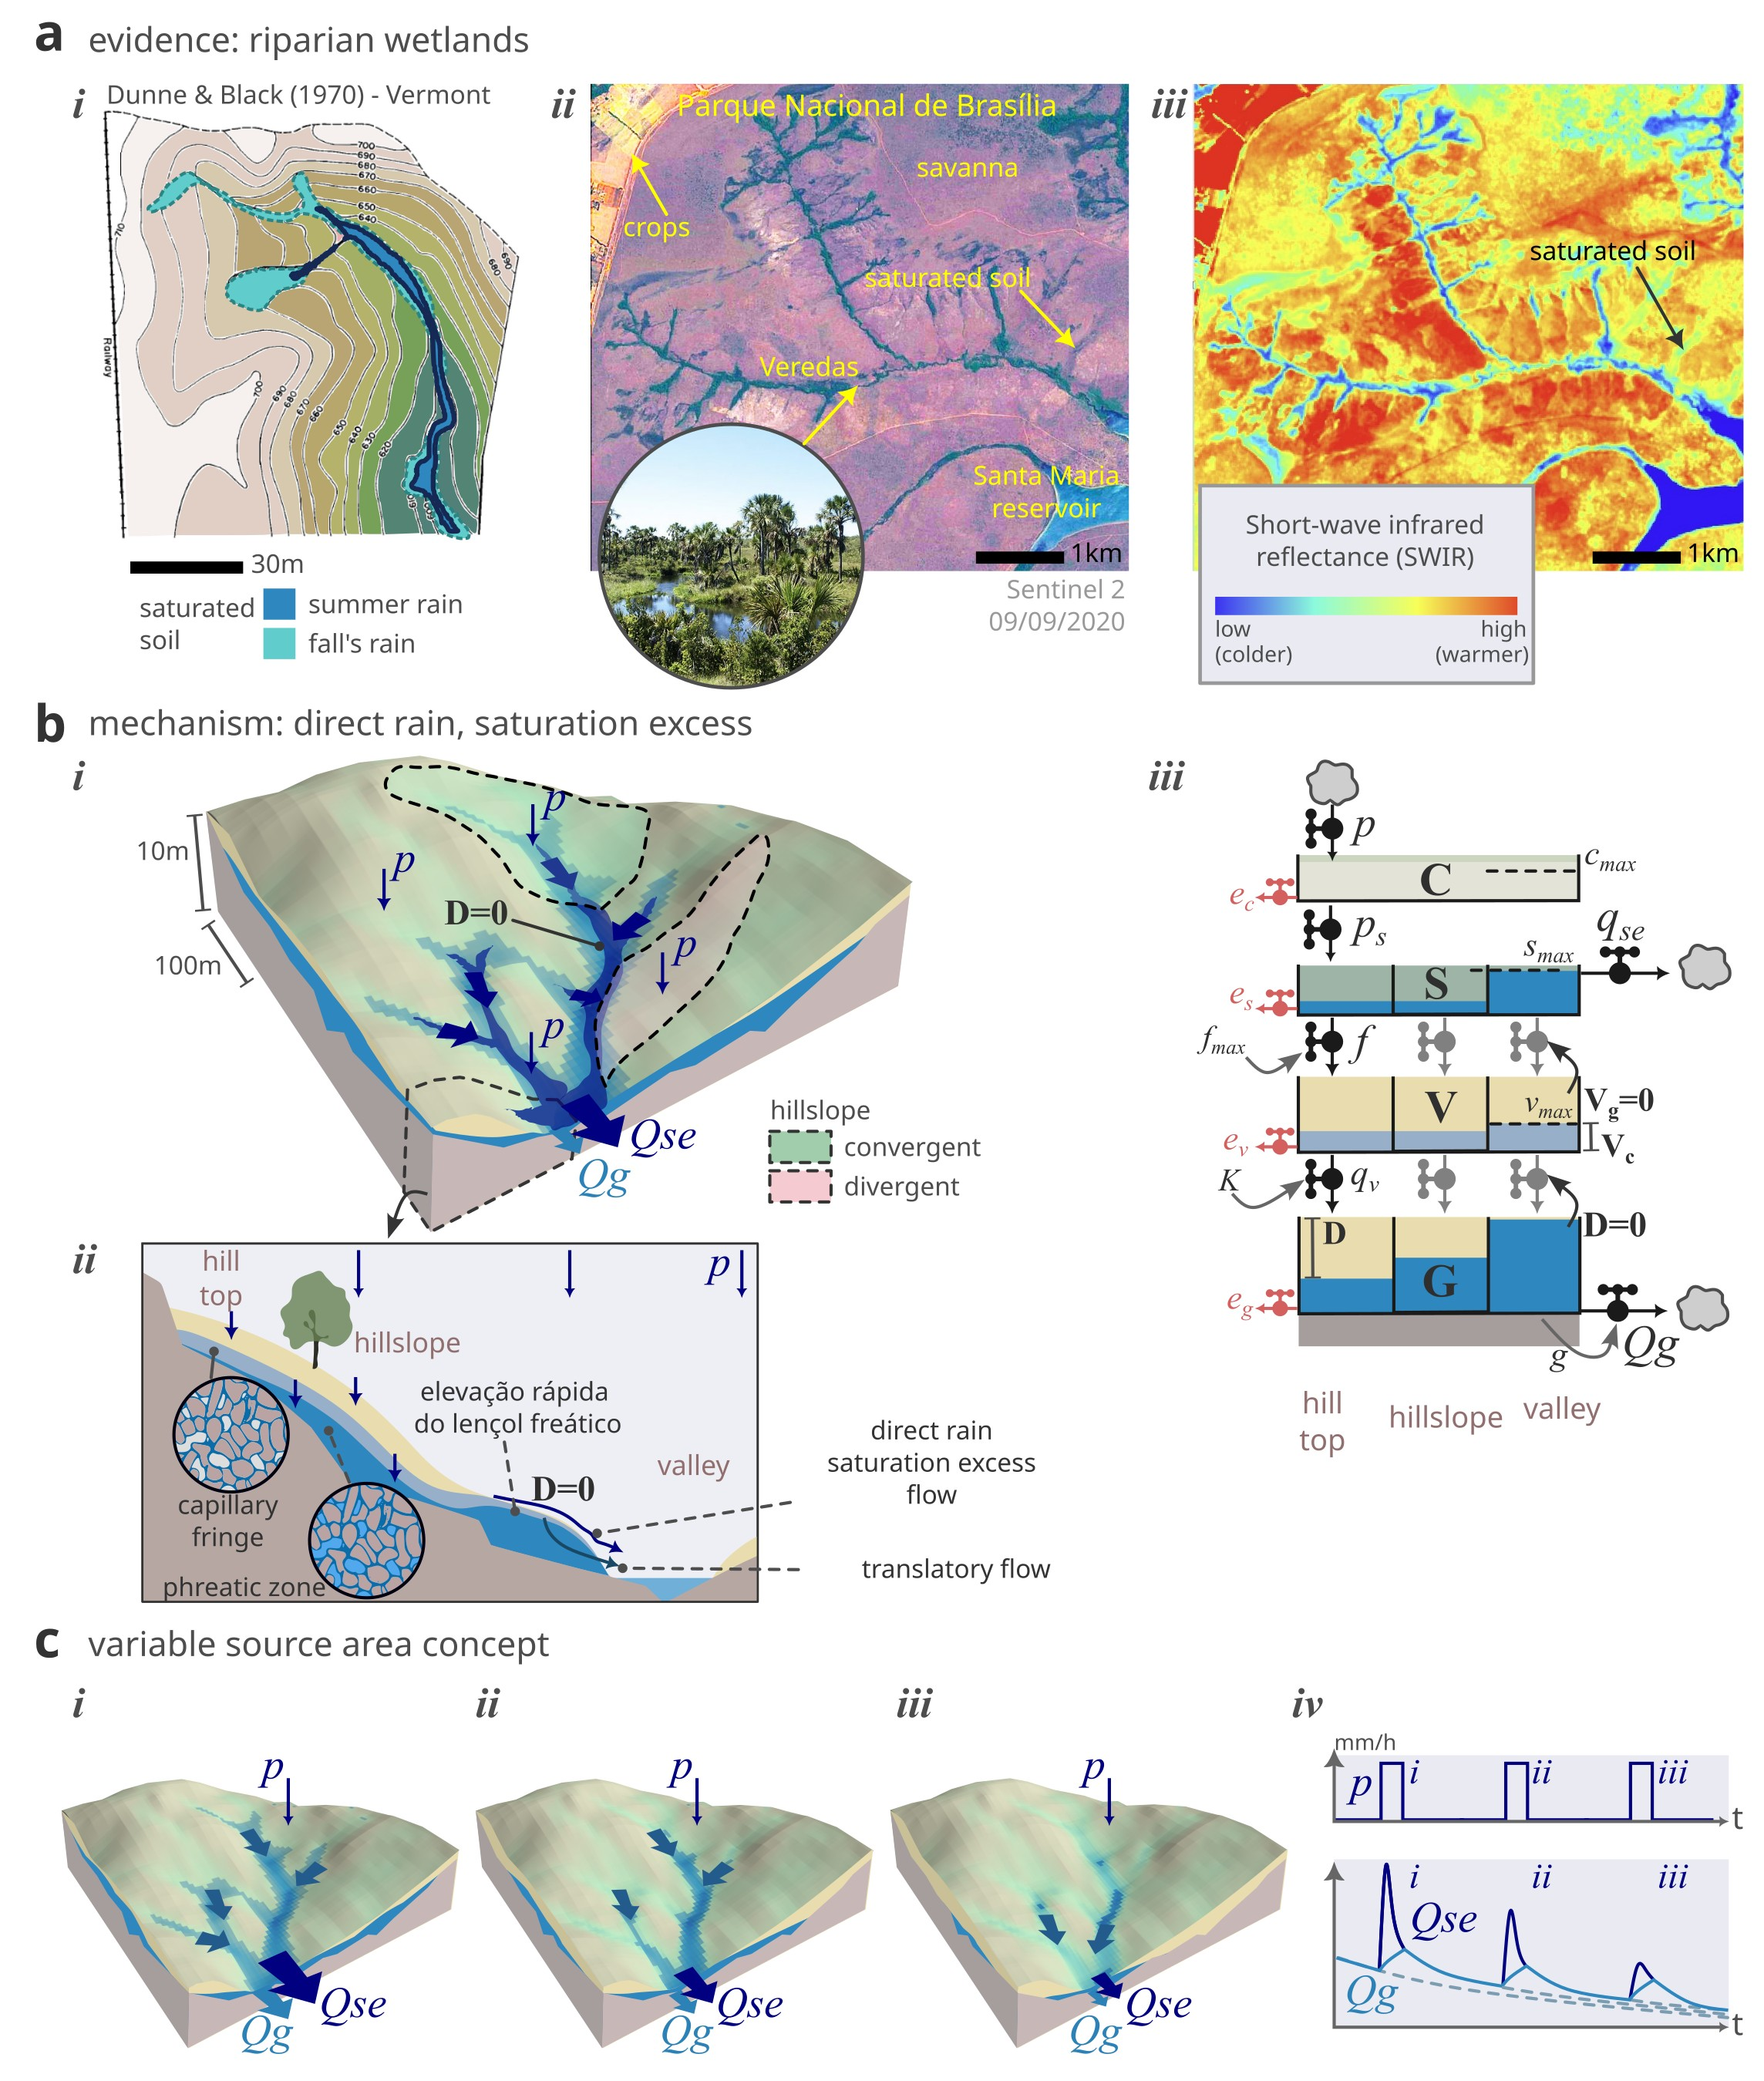
\includegraphics[width=0.98\linewidth]{figs/fig_topo_en.jpg}		
\caption[Topography and variable contributing area]
{\textbf{---\;Topography and the \gls{vsa}.}
    Topography plays a crucial role in the formation of \gls{sat_areas} that vary in extent during rainfall and throughout the seasons. These saturated soil areas thus produce \gls{rse}, as well as rapid subsurface responses from \gls{trans_flow}.
    \;\textbf{a}\;---\;Evidence: map by Dunne \& Black (1970) in Vermont (United States), demonstrating the extent of \gls{sat_areas} at different times of the year (detail \textrm{\textit{i}}), and; wet veredas in the dry season at the Brasília National Park, observed through short-wave infrared reflectance from a Sentinel-II scene on September 9, 2020 (details \textrm{\textit{ii}} and \textrm{\textit{iii}}).
    \;\textbf{b}\;---\;Systematization of the mechanism of runoff due to saturation excess. The soil in different parts of the basin (valley bottom, hillslope, and hilltop) saturates at different rates, generating rapid responses primarily in the valley bottoms. Convergent slopes tend to produce more \gls{rse} than \gls{spurs}, where \gls{qv} and \gls{ground-flow} prevail.
    \;\textbf{c}\;---\;Schematic representation of the retraction of \gls{sat_areas} during a dry spell (seasonal dynamics). This process also exhibits ephemeral dynamics during and shortly after rainfall events. Source of the photograph in \textbf{b}: https://commons.wikimedia.org/wiki/File:Veredas.jpg .
}
\label{fig:hydro:topo} 		
\end{figure}

\par The Hortonian \gls{paradigma} has not only been refuted by the recognition of \gls{subsur_flow}, as empirical evidence has also accumulated to support the existence of two additional, less intuitive rapid response mechanisms occurring in \textbf{\gls{sat_areas}}. These mechanisms, illustrated in Figure \ref{fig:hydro:topo}, result from the interaction of rain with a shallow and dynamic groundwater table, one being \gls{rse}, and the other \gls{trans_flow} (details in the next section). Both are interrelated, are strongly controlled by the terrain's topography, and also have consequences for the manifestation of \gls{subsur_flow} in macropores, as we will see later. The first of these emerges in the literature when direct precipitation in the area surrounding channels and springs is cited by Hursh \& Brater (1941) \cite{Hursh1941} as one of the sources of river runoff in the basins of the Coweeta Experimental Forest:  

\begin{adjustwidth}{100pt}{0pt}
\medskip
\small Contributions from areas of normally shallow water-tables located in close proximity to the stream, and occurring in soil-profiles which are quickly saturated. Where such conditions occur along a stream, it is expected that there will be an actual increase in the width of the channel and subsequent increase in the amount of channel-precipitation. Areas of high water tables adjacent to spring-heads would be expected to contribute similarly. -- Hursh \& Brater (1941, p. 870) \cite{Hursh1941}.
\medskip
\end{adjustwidth}

\noindent This is certainly one of the pioneering descriptions of the concept of \textbf{\gls{vsa}}: the generation of \gls{sf-runoff} as a function of the \textit{expansion and contraction of wet areas} in valley bottoms, adjacent to streams. This mechanism, illustrated in Figure \ref{fig:hydro:topo}\textbf{c}, allows any \gls{ground-rain} to transform into \gls{ex-rain} when it falls on saturated soil areas, which helps explain the prevalence of rises even in basins with high \gls{infmax} soils (as in the case of La Grange Brook, near where Robert Horton lived \cite{Beven2004c}). This concept was well organized by Cappus (1960) \cite{Cappus1960} in a study in the Alrance Experimental Basin (315 ha, France). The author claimed to have evidence for a \say{new \gls{teoria} of surface runoff}, in which the basin area can be divided into a \textit{surface runoff zone} and an \textit{infiltration zone}. The former includes a \textit{fixed} part of impermeable areas and a \textit{variable} part of permeable areas that are nearly completely saturated with water:

\begin{adjustwidth}{100pt}{0pt}
\medskip
\small
The experimental basin can be divided into two zones \(S_r\) and \(S_i\) of variable extents: --- The runoff zone \(S_r\) of area \(A_r\) includes, on one hand, fixed extent impermeable zones (roads, paved paths, compacted dirt paths from repeated traffic of people or livestock, rocky surfaces, etc.) and, on the other hand, variable extent zones consisting of permeable land, but almost completely saturated with water. The rain that falls in the zone \(S_r\) entirely transforms into \gls{sf-runoff} or subsurface runoff. --- The infiltration zone \(S_i\) of area \(A_i\) consists of unsaturated permeable land. The sandy-textured soil, which forms the surface layers of the experimental basin, is characterized by a very high \gls{infmax} \(f\) that exceeds the intensity of all rains that may fall on this basin—except for those of extremely rare occurrence. Thus, except in very exceptional cases, the rain that falls in the zone \(S_i\) is completely absorbed by infiltration and consequently generates no runoff.
\footnote{Freely translated from: 
\textit{
Le Bassin expérimental peut être partagé en deux zones $S_r$ et $S_i$ d'étendues variables:\;--- La zone de ruissellement $S_r$ de superficie $A_r$ comporte, d'une part, des zones imperméables d'étendue fixe (routes, chemins empierrés, chemins de terre tassée par le passage répété des hommes ou du bétail, surfaces rocheuses, etc.) et, d'autre part, des zones d'étendue variable constituées de terrains perméables, mais à peu près complètement saturés d'eau. La pluie tombant sur la zone Sr se transforme entièrement en ruissellement superficiel ou hypodermique. --- La zone d'infiltration $S_i$ de superficie $A_i$ est constituée par les terrains perméables non saturés. Le sol de texture sableuse, qui forme les couches superficielles du Bassin expérimental est caractérisé par une capacité d'infiltration $f$ très forte qui dépasse l'intensité de toutes les pluies pouvant tomber sur ce bassin — à l'exception seulement de pluies d'une rareté extrême — ainsi, sauf en des cas très exceptionnels, la pluie tombant sur la zone $S_i$ est entièrement absorbée par infiltration et ne donne lieu par conséquent à aucun ruissellement.
}} -- Cappus (1960, p. 503) \cite{Cappus1960}.
\medskip
\end{adjustwidth}

\noindent Tsukamoto (1963) \cite{Tsukamoto1963} also structured a similar \gls{teoria}, based on results obtained in a basin at the University of Tokyo Forest (106.7 ha, Japan). In his paper, he points out that riparian areas exhibit rapid saturation responses due to the influence of the \textbf{\gls{fringe}} of groundwater, generating \gls{sf-runoff} in this part of the slope, as opposed to the higher and well-drained parts of the terrain. The experimental results from Ragan (1968) \cite{Ragan1968}, mentioned above, also demonstrated rapid rises in the water table near the stream during monitored rainfall events. Even Betson (1964) \cite{Betson1964}, while attempting to uphold the Hortonian \gls{percept-model}, noted that half of the runoff was possibly generated by a swamp area in one of the basins analyzed in his study.

\par To corroborate the \gls{teoria} of \gls{vsa}, Dunne \& Black (1970) \cite{Dunne1970, Dunne1970b} published detailed results for a small experimental basin in Vermont (United States). In this study, the authors present maps of saturated soil areas that follow the terrain's channel (detail \textit{i} in Figure \ref{fig:hydro:topo}\textbf{a}), which showed variations both throughout the year (seasonal dynamics) and during rainfall events (ephemeral dynamics). The seasonal dynamics of these wet areas is explained by the increase in \gls{qv} of groundwater during the wetter season, which expands the extent of spring emergence zones in the valley bottoms. Detail \textit{ii} in Figure \ref{fig:hydro:topo}\textbf{a} demonstrates evidence of seasonal dynamics from short-wave infrared (\texttt{SWIR}) reflectance with a Sentinel-II scene on September 9, 2020, in the Brasília National Park. This period is marked by dry conditions, but the riparian areas remain moist, forming the Veredas. On the other hand, the ephemeral dynamics are explained by a rapid rise of the \gls{sat-zone} when the \gls{fringe} is very close to the surface (more details ahead).

\par The unequivocal observation of the dynamics of saturated areas by Dunne \& Black (1970) solidified the perception that \textit{topography} exerts an important control in the \gls{hydrology} of zero-order basins, and not just the \textit{surface} of the soil, as postulated by the infiltration \gls{paradigma}. In this sense, Anderson \& Burt (1978) \cite{Anderson1978} demonstrated that, in a basin in the Quantock Hills (England), the rapid rise of the water table along the channels of the \textbf{\gls{hollows}} is much greater than in the \textbf{\gls{spurs}}. The former tend to generate relatively more \gls{rse} and also more \gls{subsur_flow}, as the sudden rise of groundwater activates the macropore network in the soil. In the \gls{spurs}, on the other hand, slower processes of \gls{qv} and \gls{ground-flow} predominate. 

\par In this context, the mechanism of \gls{sf-runoff} defended in Horton’s \gls{teoria} (infiltration excess) was not exactly refuted but reserved as a response mechanism limited to extraordinary precipitation events or areas with altered soil, whether in natural environments (such as rocky outcrops and arid regions) or anthropized environments (such as agriculture and urban areas). This implies that the use of the \acrshort{cn} method from the \acrshort{scs} is justified when its application is directed towards extreme rainfall events or in urban and rural basins where the Hortonian mechanism is clearly dominant. However, this restriction is not explicitly stated in the official manuals of the method, which also include \acrshort{cn} values for forests and other natural land covers. Additionally, simulation models such as \texttt{SWAT} and \texttt{SWMM} utilize continuous simulation (various rainfall events) and represent any land cover. It is worth noting that Horton (1936) \cite{Horton1936} came close to analytically deducing this mechanism in one of his papers, as he highlights that sloping soil hillsides induce the water table to intercept the surface above the valley bottom level, causing the emergence of a saturated surface in this convergent part of the topography \cite{Beven2004b}.

\subsection{The water age paradoxes}

\begin{figure}[t!] 
\centering				
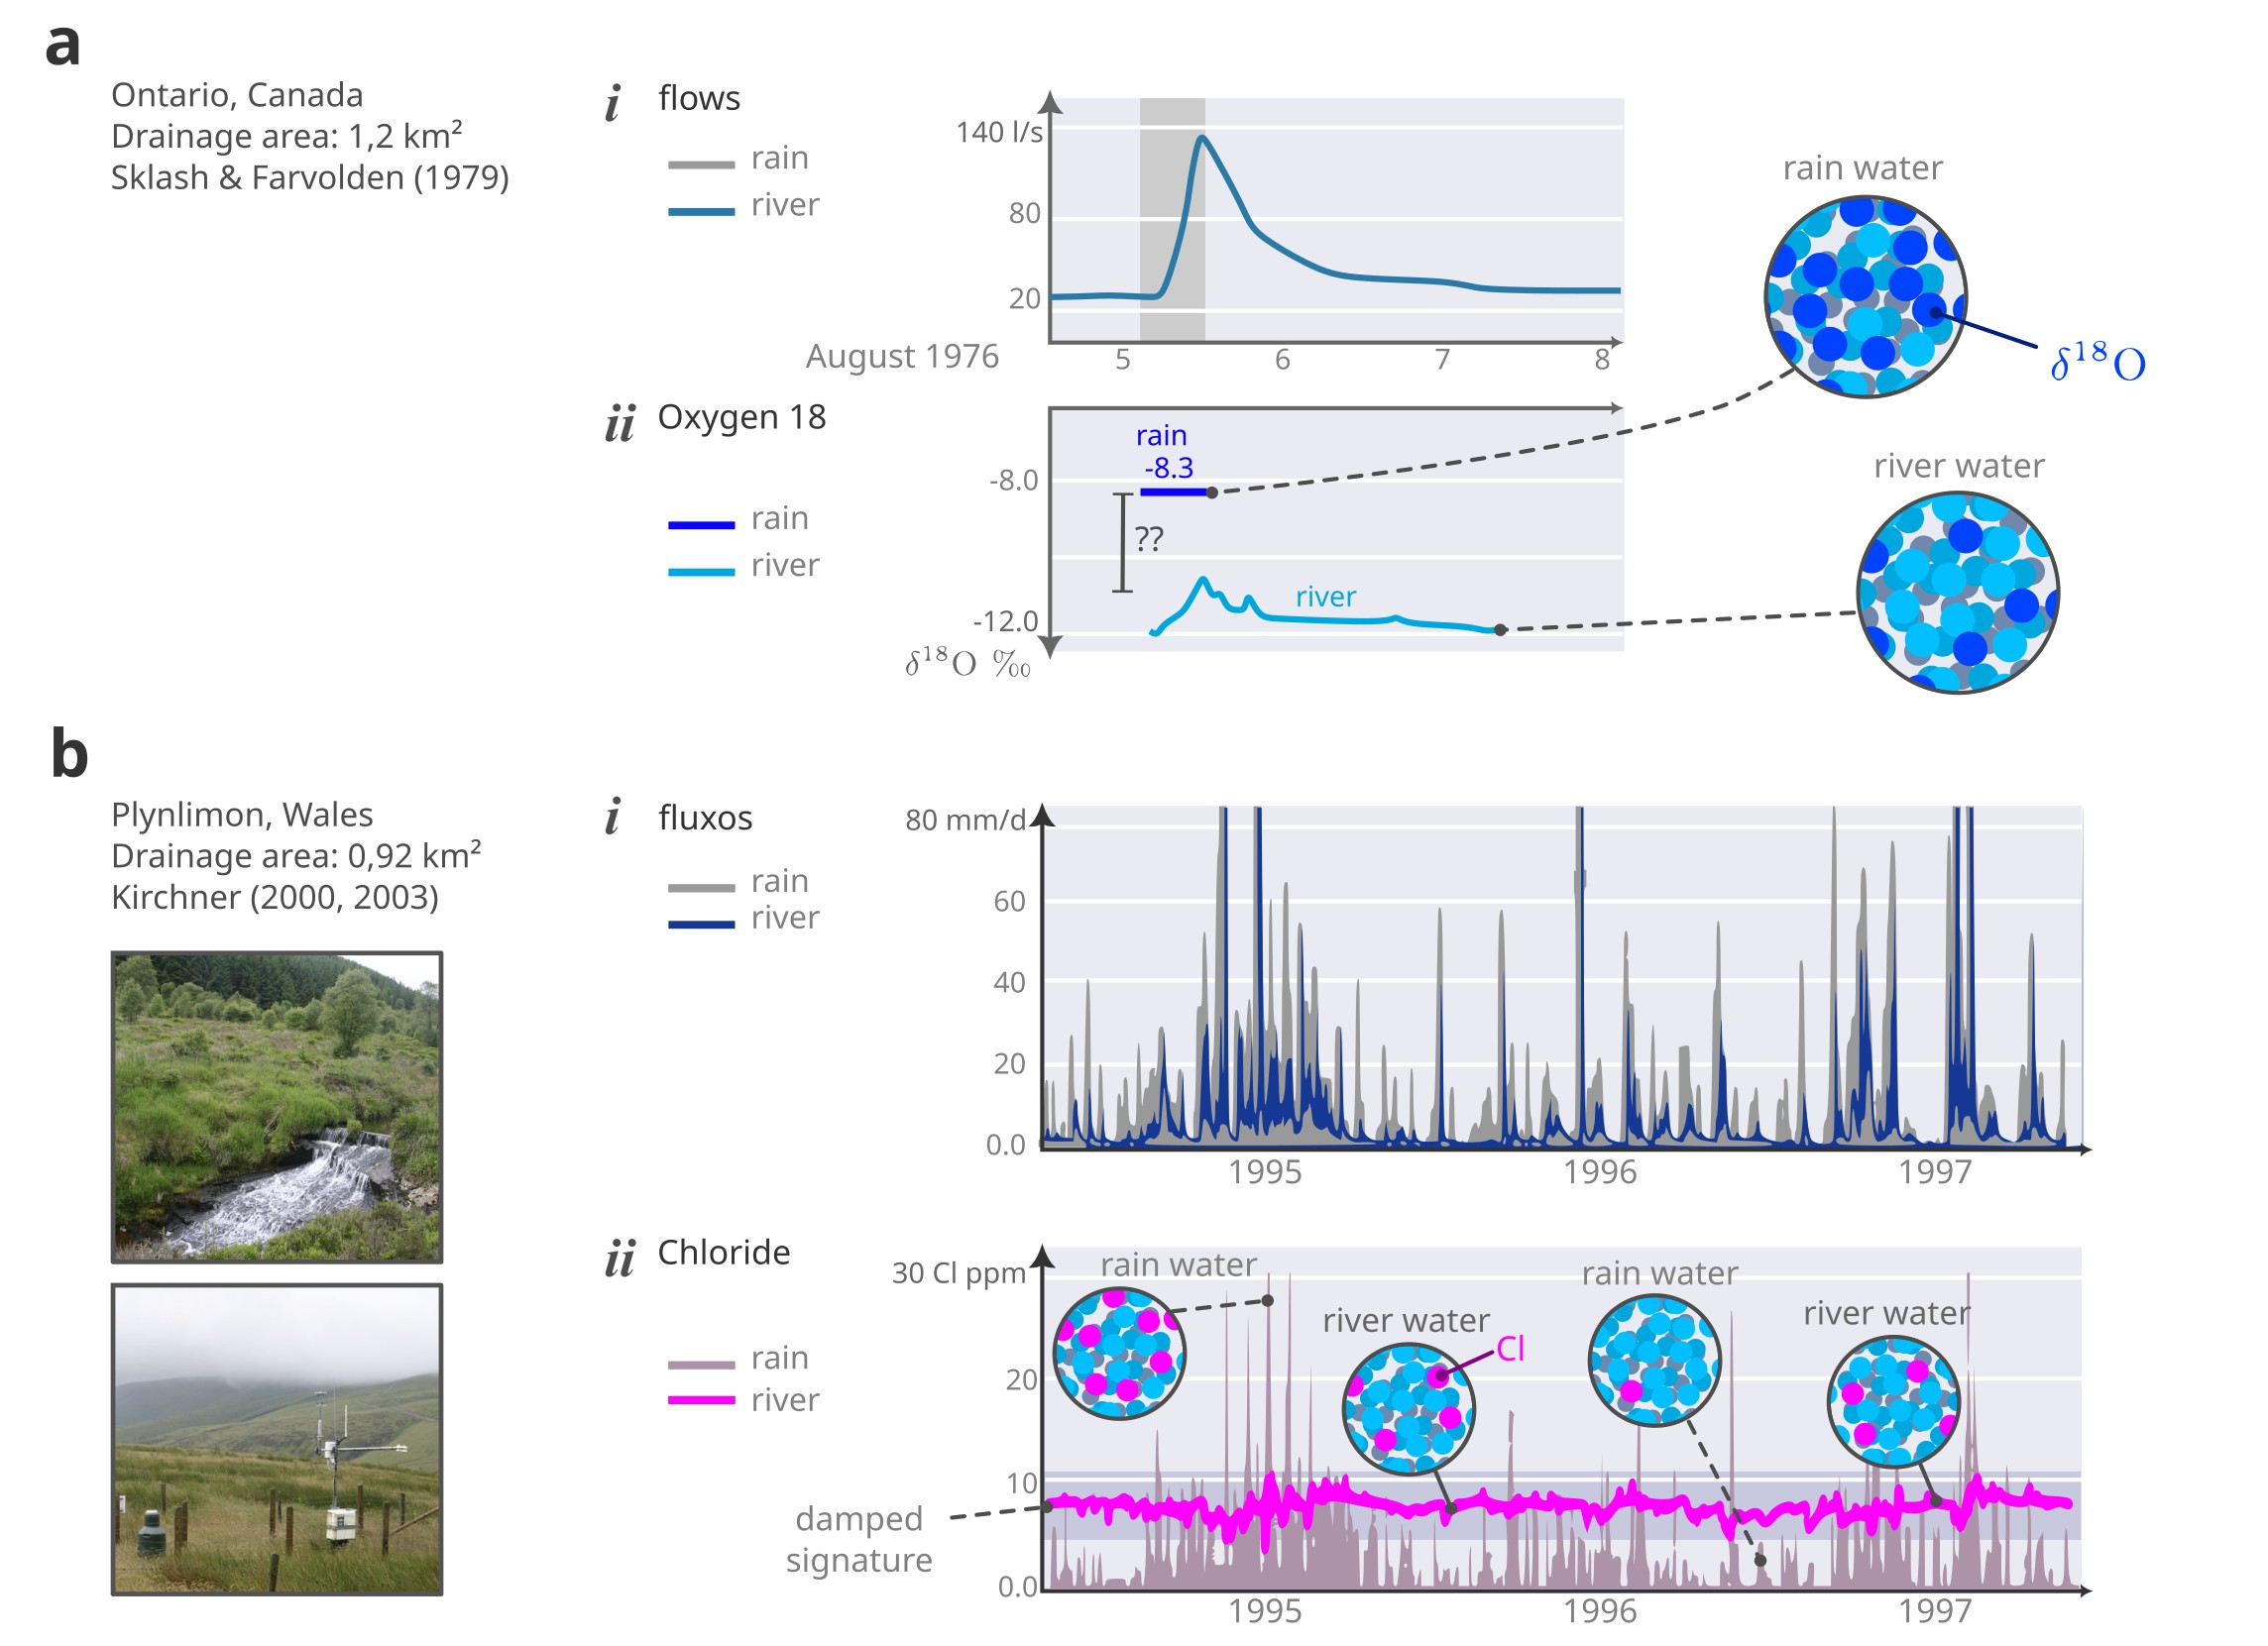
\includegraphics[width=0.98\linewidth]{figs/fig_paradox2_en.jpg}		
\caption[The old water paradox]
{\textbf{---\;The \gls{old_water_paradox}.}
    Analyses of \gls{iso_sign} and geochemistry of rainwater and river water during rises make it clear that they are waters of different ages, thus creating a paradox. \;\textbf{a}\;---\;Evidence provided by Sklash \& Farvolden (1979) \cite{sklash1979} in a rural basin in Ontario, Canada (1.2 km² drainage area). The flows clearly denote a rapid response from the basin (flood) to the rainfall event (detail \textrm{\textit{i}}). However, the \gls{iso_sign} with Oxygen-18 shows that the water in the flood is not the same as the rainwater (detail \textrm{\textit{ii}}).\;\textbf{b}\;---\;The same paradox observed with Chloride (marine aerosol) by Kirchner \textit{et al.} (2000, 2003) \cite{kirchner2000, Kirchner2003} in an experimental basin in Plynlimon, Wales (0.92 km² drainage area). The flows are typical rapid responses (detail \textrm{\textit{i}}), but the river signature shows a pronounced damping over the years, suggesting a long-duration mix (detail \textrm{\textit{ii}}). Source of the photographs: Ecological Continuity Trust \cite{ect_plynlimon}.
}
\label{fig:hydro:paradox2} 		
\end{figure}

\par Translational subsurface runoff, in turn, is conceptually speculated by Hewlett \& Hibbert (1967) \cite{Hewlett1967}, in a clearly revolutionary article in the field of \gls{hydrology} \cite{McDonnell2009}. While criticizing the hegemonic \gls{paradigma} of the time (the infiltration capacity \gls{teoria}), the authors organize new relevant concepts, such as the terms \say{rapid and slow responses} and \say{variable contributing area}, paving the way for the advent of the new \gls{paradigma}. In this direction, the authors suggest a mechanism of \textit{instantaneous} subsurface response that occurs when the \gls{fmc} of the soil is exceeded by the infiltration of rainwater in the riparian zones, where there is greater influence from capillarity fringes. In summary, they postulate that this response, although rapid, would not exactly be rainwater but water that had settled in the soil matrix \textit{before} the event occurred. In this process, the thickness of water films on soil particles in the \gls{unsat-zone} suddenly reaches a limit where the pore network becomes pressurized by gravity. Therefore, the \textbf{new water} from the rain (event water) triggers a pulse, a pressure wave, that expels the water stored in the soil at the base of the slope, referred to as \textbf{old water} (pre-event water):

\begin{adjustwidth}{100pt}{0pt}
\medskip
\small
However, of the part contributed to direct runoff, a fraction will be some of the actual drops that fell during the storm -- that is, some new rain -- and the other fraction will be what we might call translatory flow, or flow produced by a process of displacement. This is a contribution to direct flow of water already stored in the soil mantle before rainfall began. It will be released in large quantities only when the soil is within field capacity range or wetter. Above the zone of saturation, we may regard such movement as due to thickening of the water films surrounding soil particles and a resulting pulse of water flux as the saturated zone is approached. -- Hewlett \& Hibbert (1967, p. 279) \cite{Hewlett1967}.
\medskip
\end{adjustwidth}

\par Although the \gls{teoria} makes sense and cites laboratory studies, the text by Hewlett \& Hibbert (1967) does not provide empirical evidence obtained in the field to justify the reality of this mechanism. However, this gap was filled by Pinder and Jones (1969) \cite{pinder1969}, who evaluated the separation of flood hydrographs in three monitored basins in Nova Scotia (ranging from 647.5 ha to 13.5 km², Canada). Unlike conventional graphical methods, they inferred the separation between \gls{sf-runoff} and subsurface flow using chemical tracers and a simple mass balance \gls{model}\footnote{The developed \gls{model} consists of two mixing compartments: $C_{tr}Q_{tr} =C_{dr}Q_{dr} + C_{gw}Q_{gw}$, where: $C$ is the concentration of some conservative solute; $Q$ is the flow; $tr$ denotes total flow; $dr$ denotes direct runoff, and; $gw$ denotes groundwater flow.}. In the presented case, sodium, calcium, bicarbonate, magnesium, and sulfate concentrations were monitored before and during flood events. The results indicated a substantial prevalence of groundwater flow during rises, accounting for 32\% to 42\% of the maximum hydrograph flow. However, this did not eliminate the alternative explanation of a subsurface response from rainwater (new water) that dissolved the monitored solutes while rapidly moving through the soil. Evidence in favor of groundwater (old water) became much more robust with the advent of hydrogen and oxygen isotope monitoring, such as Deuterium ($^{2}\text{H}$), Tritium ($^{3}\text{H}$), and Oxygen-18 ($^{18}\text{O}$), which are ideal markers that are part of the water molecule itself\footnote{Unlike common solutes, the concentration of $^{18}\text{O}$ is measured by the difference in parts per thousand ($\delta^{18}\text{O}$ ‰) of the ratio of $^{18}\text{O}/^{16}\text{O}$ of a standard and the sample: $\delta^{18}\text{O} = (\frac{^{18}\text{O}/^{16}\text{O} \,\text{sample}}{^{18}\text{O}/^{16}\text{O}\,\text{standard}} - 1) \times 1000$. The standard is usually the mean ocean water (\texttt{SMOW}). Waters depleted of $^{18}\text{O}$ relative to the standard exhibit negative $\delta^{18}\text{O}$, and vice versa.}. In locations with significant variability in the \textbf{\gls{iso_sign}} of the precipitated water, it is possible to estimate how much of this new water is present during rises\footnote{Obviously, if the rainwater is isotopically indistinguishable from the river water just before the event, then it is impossible to extract any relevant information.}. This strategy was suggested by Dinçer et \text{al.} (1970) \cite{dincer1970} in a study in the mountains of Czechoslovakia that demonstrated the effect of \textbf{\gls{term_frac}}\footnote{The main cause of the fractionation of these isotopes in the atmosphere arises from the difference in vapor pressure between isotopically heavy and light water molecules: ${\text{H}_{2}}^{18}\text{O}$ has a lower vapor pressure than ${\text{H}_{2}}^{16}\text{O}$ and, therefore, ${\text{H}_{2}}^{16}\text{O}$ remains preferentially in the liquid phase during both evaporation and condensation processes. Thus, the observed concentrations of $\delta^{18}\text{O}$ in precipitation tend to be incrementally negative as moist air masses move over continents \cite{sklash1976}.} on the concentrations of $^{3}\text{H}$ and $^{18}\text{O}$ in snow layers that precipitated and melted over the seasons. Subsequently, the results published by Martinec et \text{al.} (1974) \cite{martinec1974} noted that river water in the Swiss mountains exhibited a relatively low variability in $^{18}\text{O}$ concentration, approaching the long-term average of seasonal oscillations observed in precipitation. The strategy then took on well-defined contours with the article by Sklash et \text{al.} (1976) \cite{sklash1976}, which, in addition to organizing the logic of the method, showed that in two monitored basins in Ontario (Canada), the contribution of groundwater to the maximum flood flow ranged from 55\% (in upstream basins) to 70\% (in downstream basins draining an area of 700 km$^2$). These results carry revolutionary implications:

\begin{adjustwidth}{100pt}{0pt}
\medskip
\small
The most important finding is that the pre-storm component of storm runoff for the 16 May storm was large. For example, at peak total discharge, the pre-storm component of Big Otter Creek at Vienna was 70 $\pm$ 9\% of storm runoff. These results substantiate the findings of Pinder \& Jones (1969) and Fritz \textit{et al.} (1974), even though the basins in the present study are one to two orders of magnitude larger in areal extent.These results are not consistent with the simulated results of Freeze (1972b), the field results of Dunne \& Black (1970a,b), and Hewlett \& Hibbert (1967), or the theoretical implications of Horton (1933). The results are particularly encouraging, though, in light of the large subsurface (prestorm) component of snowmelt noted by Dinçer \textit{et al.} (1970). -- Sklash et \text{al.} (1976, p. 276) \cite{sklash1976}.
\medskip
\end{adjustwidth}

\noindent Michael Sklash continued studies of this type, corroborating the existence of this process in basins in Canada, New Zealand, and the British Isles \cite{sklash1979, sklash1986, sklash1996}. For example, the article by Sklash \& Farvolden (1979) \cite{sklash1979} in Canada presents similar results for a basin with intensive agriculture (1.2 km², in the Hillman Creek Experimental Basin, Ontario, Figure \ref{fig:hydro:paradox2}\textbf{a}) and two highly forested basins (1.0 km² and 3.9 km², in the Ruisseau des Eaux Volées Experimental Basin, Québec). In addition to reporting the surprising prevalence of old water in rises (between 80\% to 94\% of total runoff), the authors contribute to the \gls{teoria} of rapid rises in groundwater in valley bottoms to explain the phenomenon. In the MaiMai Experimental Basin (New Zealand), Sklash et \text{al.} (1986) \cite{sklash1986} present results that drastically revise the interpretations of Mosley (1979) \cite{Mosley1979}. As mentioned above, Mosley (1979) argues for the dominance of \gls{subsur_flow} (new water) in this basin. The unequivocal prevalence of old water in rises, obtained with isotopic markers, created a certain impasse in the \gls{comunidade-cientifica}, which since then has proposed plausible mechanisms \cite{buttle1994}. In this context, McDonnell (1990) \cite{mcdonnell1990} synthesizes the response mechanisms in the MaiMai basin, introducing the concept of \textbf{activation of subsurface flow} from the entry of rainwater into the macropore network of the hillslopes, i.e., through \gls{subsur_flow}. In this scheme (illustrated in Figure \ref{fig:hydro:paradox}\textbf{a}), he emphasizes the role of \textit{vertical} shortcuts in the soil profile, created by macropores, which allow the new rainwater to rapidly lodge in the capillary fringes of the \gls{sat-zone}, thereby activating the hydraulic head necessary to quickly expel the old groundwater at the base of the slope. A new review by McGlynn et \text{al.} (2002) \cite{mcglynn2002} also highlights the relevant effect of the \textbf{\gls{bedrock_topo}} of the slope (the underlying relatively impermeable bedrock). It is suggested that the irregularities of this layer can create \textbf{stagnation zones} or \textbf{pockets} that store water underground for much longer than expected. The eventual hydraulic activation of these relatively inaccessible parts expels old water at the base of the slope, facilitated by the presence of macropores. Indeed, the influence of underlying geological structures (fractures) on the emergence of groundwater had already been mentioned by Huff et \text{al.} (1982) \cite{Huff1982}, but without analyzing the age of the water using isotopes.

\begin{figure}[t!] 
\centering				
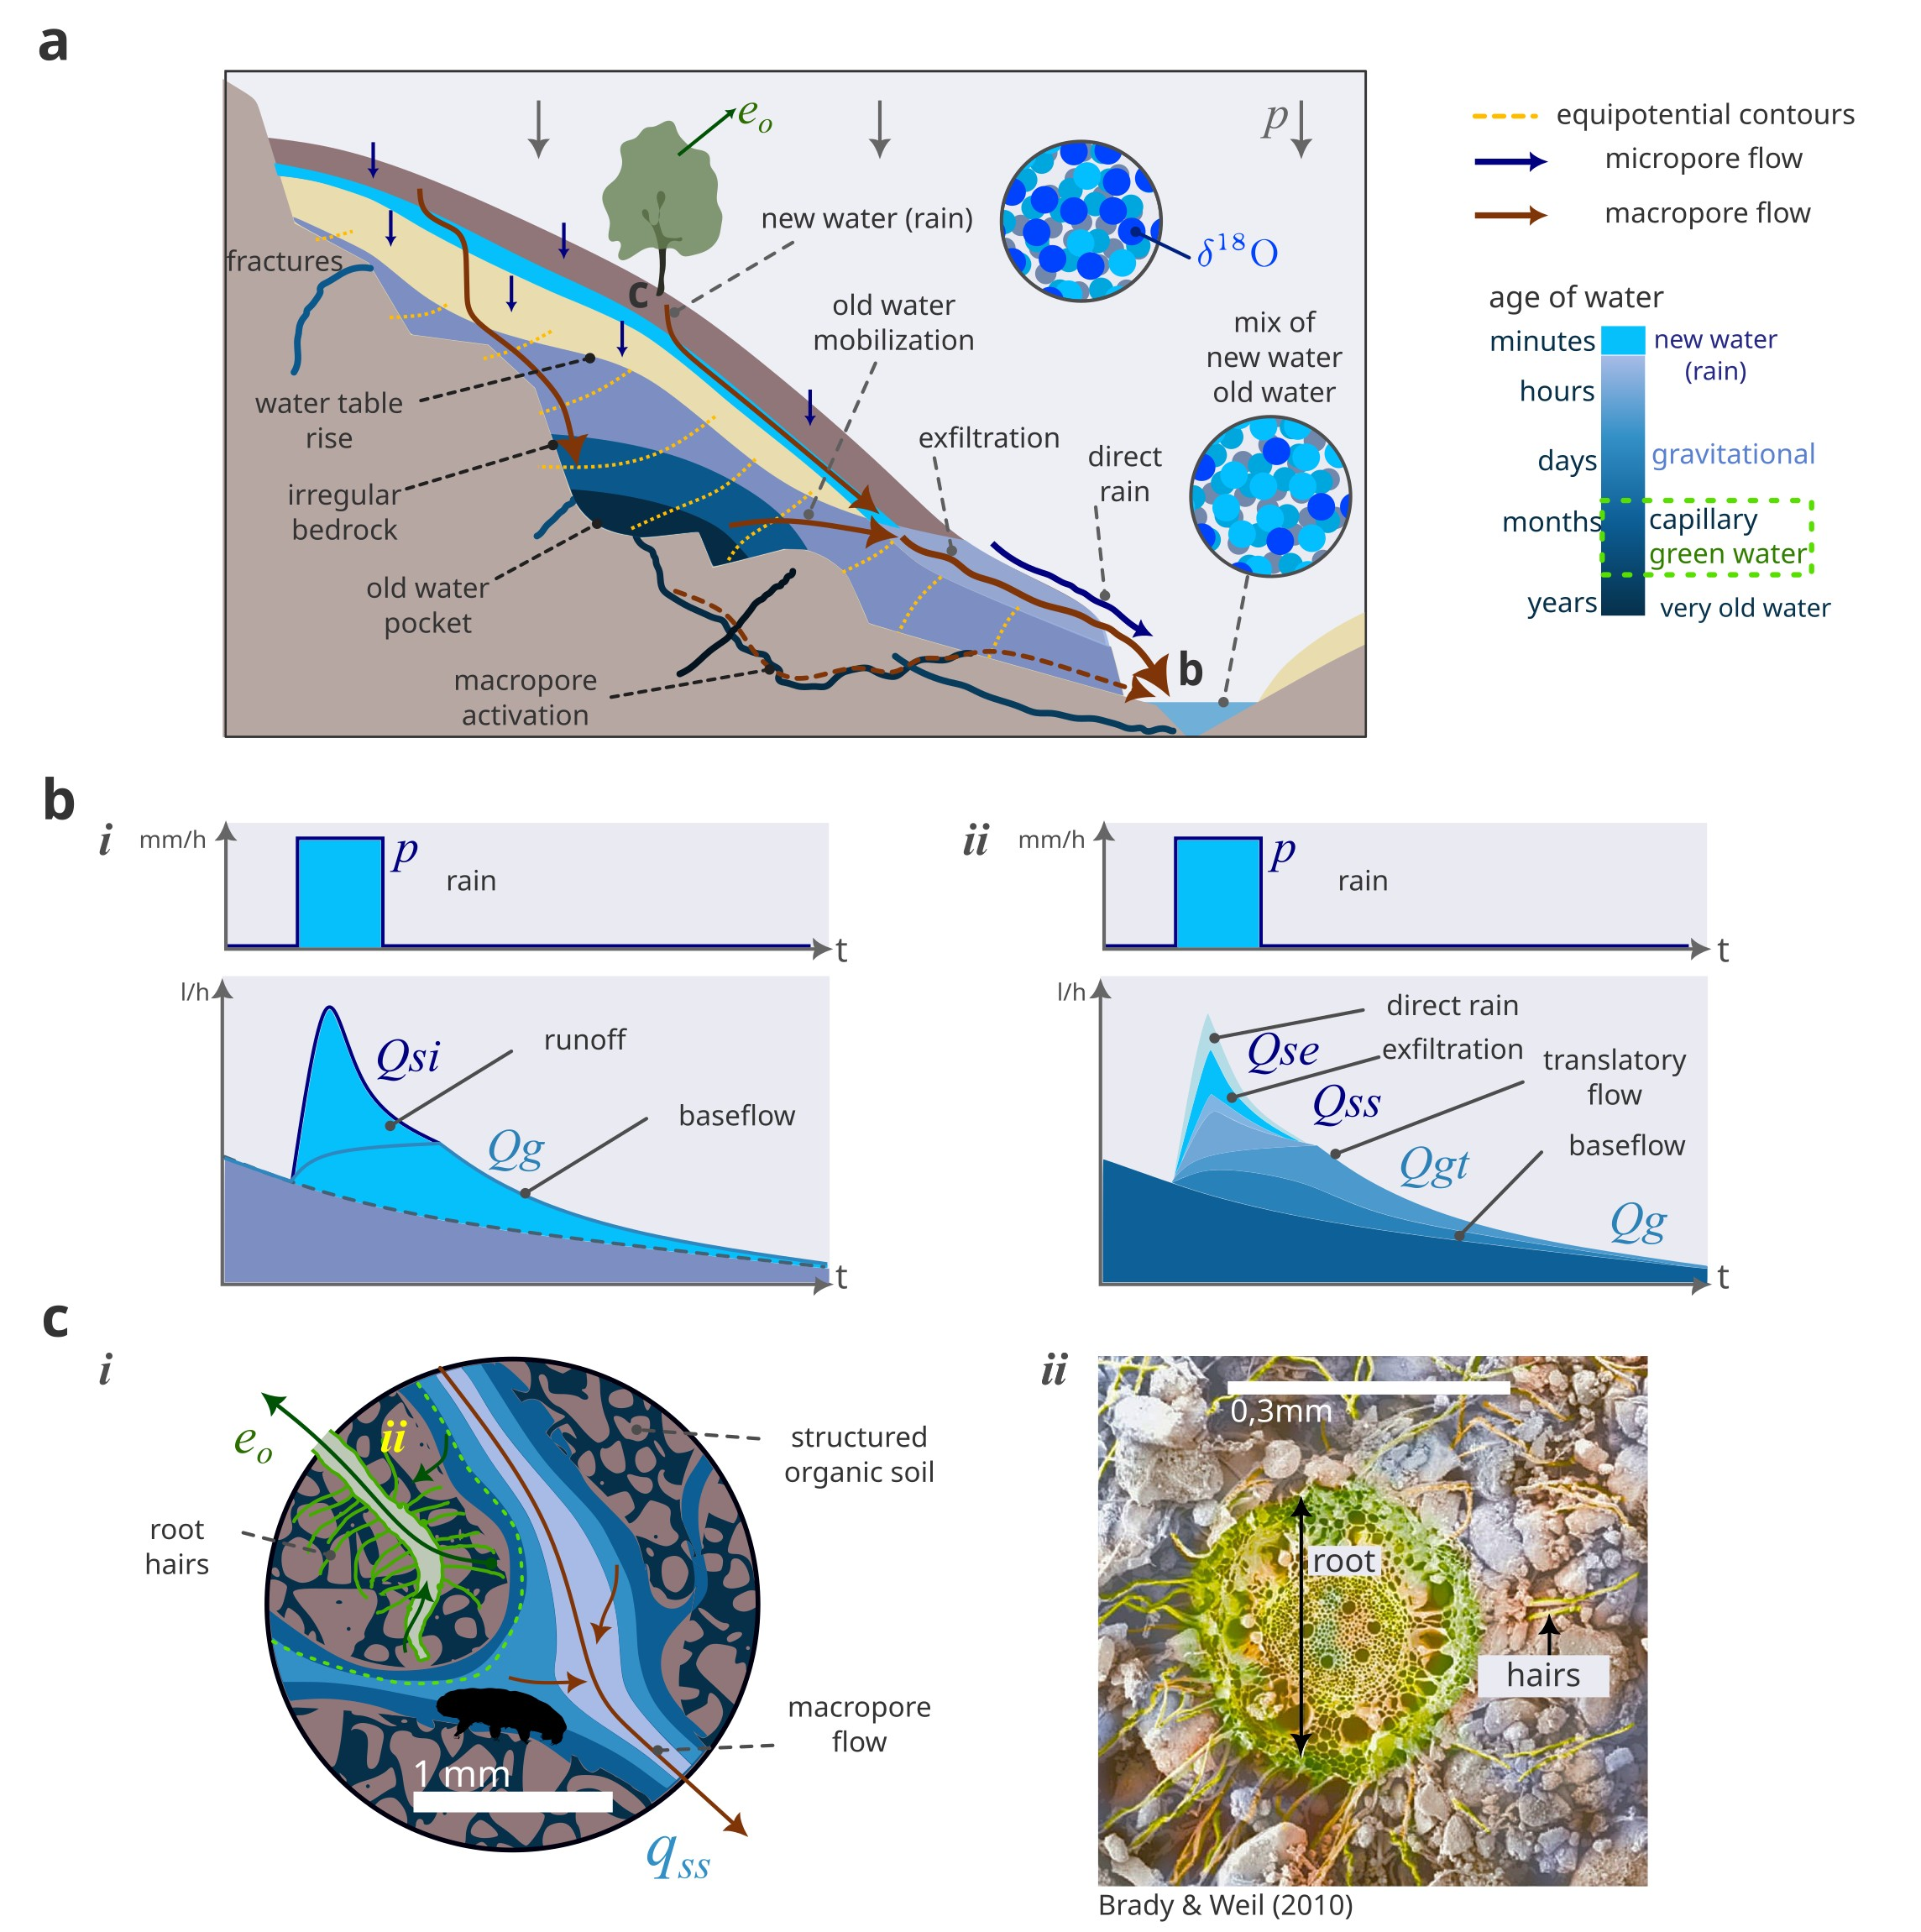
\includegraphics[width=0.98\linewidth]{figs/fig_paradox_en.jpg}		
\caption[Mobilization of old water]
{\textbf{---\;Mobilization of old water.}\;\textbf{a}\;---\;The rise of the water table combined with flow through macropores (fractures and preferential pathways) helps explain the dominance of old water in the rapid responses of rivers. Vertical shortcuts allow new water (rain) to mix with older water in stagnation zones (pockets) at the aquifer's threshold, activating hydraulic head in fractures and preferential pathways, resulting in the rapid expulsion of old water.\;\textbf{b}\;---\;Differences between the Hortonian \gls{model} of rapid response (Type 3 flood) and the \gls{model} obtained from isotopic analyses.\;\textbf{c}\;---\;Water in the soil also shows an age differentiation, which is perceived in the evapotranspiration flows of plants (detail \textrm{\textit{i}}). The \gls{water_capilar} is absorbed by fine roots, while \gls{water_gravit} drains to the base of the slope (detail \textrm{\textit{ii}}). Photograph from electron microscopy adapted from Brady \& Weil (2010) \cite{brady2010}. 
}
\label{fig:hydro:paradox} 		
\end{figure}

\par The evidence, impasses, and plausible mechanisms proposed to explain the dominance of old water in rapid responses further increase in complexity given the results of \textbf{\gls{geo-sign}}, which tend to exhibit high variability. In this sense, Burns et \text{al.} (2001) \cite{burns2001quantifying} suggest that the surface responses in the Panola Mountain Experimental Basin (Georgia, United States) end up mixing with groundwater in the riparian zone before entering the channels. Seibert et \text{al.} (2003) \cite{seibert2003groundwater} also emphasize the difference in \gls{geo-sign} between the water in the riparian zone (anoxic conditions) and the water in well-drained hillslope soils (greater aeration). This complexity has led to some perplexity, expressed by Kirchner (2003) \cite{Kirchner2003} in the so-called \textit{double paradox of catchment hydrology and geochemistry}, or simply \textbf{\gls{old_water_paradox}}. For him, this paradox has two components that, although related, are somewhat contradictory: (1) \gls{hydrology}: the rapid mobilization of old water—the quick replacement of old water by new, as postulated by \gls{trans_flow}, and; (2) Geochemistry: the chemical variability of old water—the fact that old water assumes different chemical signatures depending on the flow velocity. In this sense, based on chloride concentrations\footnote{An analogous strategy to that used with isotopes is possible in basins with marine aerosol deposition, with chloride being an inert marker that can be analyzed in rainwater.} monitored in a basin in Wales, Kirchner et \text{al.} (2000) \cite{kirchner2000} propose a \textbf{\gls{geo_hydro_sep}} of the soil, where pores and fractures exhibit a fractal structure of residence times (see Figure \ref{fig:hydro:paradox2}\textbf{b}). This implies why the slopes of the basins transmit \textit{hydrological signals} much faster than \textit{geochemical signals}. This concept becomes clearer through Iorgulescu et \text{al.} (2007) \cite{Iorgulescu2007}, who reinforce the difference between the \textit{wave} speed (\textbf{celerity}) of water and the \textit{molecular} speed of water—beyond material, flood flow is an energy flow. In the same spirit, McDonnell (2014) \cite{mcdonnell2014} also draws a new perspective on evapotranspiration flows, particularly regarding the age of the water that plants consume, proposing the possibility of a \textbf{\gls{eco_hydro_sep}} of the soil, which he refers to as \textbf{\gls{two_world}}. In this situation, the water consumed by the roots and \textbf{fine roots} of plants (known as \textit{green} water) would be \gls{water_capilar}, relatively older than \gls{water_gravit} (see Figure \ref{fig:hydro:paradox}\textbf{b}). Evaristo et \text{al.} (2015) \cite{Evaristo2015} provide evidence supporting this \gls{hipotese}, showing that ecological separation is common in various biomes—plants use soil water with an \gls{iso_sign} distinct from the water contributing to the \gls{qv} of groundwater and to river runoff.

\section{Limitations of hydrological models} \label{sec:hydro:others}

\par Accompanying the scientific revolution brought about by empirical evidence regarding runoff mechanisms on hillslopes, the 1960s was also marked by the advent of the first hydrological models simulated on digital computers. This occurred largely due to a confluence of factors, such as the intellectual context of von Bertalanffy's General Systems Theory and the practices of Jay Forrester's \gls{sys-dyn}, following the emergence of digital mainframe computers. Keith Beven reports that by 1971, he had counted over a hundred hydrological models in the literature, which were basically versions of the Stanford University \gls{model}, the \textit{Stanford Watershed Model IV} (\texttt{SWM}) \cite{Beven2019a}. The \gls{model} was developed starting in 1959 as Norman Crawford's doctoral thesis, supervised by Ray Linsley, and later gave rise to a program called the \textit{Hydrologic Simulation Program, Fortran} (\texttt{HSPF}), developed for and with the support of the U.S. Environmental Protection Agency (\texttt{USEPA}) \cite{Burges2004a}. This pioneering \gls{model} clearly exemplifies the influence of the ontology offered by \gls{sys-dyn}: a network of reservoirs connected by flows that is solved numerically. In this case, the SWM is only slightly more intricate than the minimalist \gls{model} presented in the previous chapter, with four reservoirs (canopy, \gls{unsat-zone}, \gls{sat-zone}, and drainage channels) and three response mechanisms (including a subsurface response in addition to \gls{sf-runoff} and groundwater flow). However, the \gls{model} does not represent water storage on the surface, nor does it differentiate topographic aspects in a way that surface runoff can be separated into \gls{sf-runoff} or \gls{rse}. But this is not exactly a problem in \gls{sys-dyn}; it is sufficient to add a new compartment and connect the flows. The flexibility provided by \gls{sys-dyn}, in this sense, introduced it as a conceptual and procedural \gls{paradigma} in hydrological modeling, resulting in both a proliferation of models from this period and an increased theoretical understanding of the importance of \textbf{scale} throughout the modeling process.

\subsection{On data and processes} \label{sec:hydro:databased}

\par Before the advent of hydrological simulations, however, the approach to obtaining flood hydrographs from rainfall data primarily relied on the concept of \textbf{\gls{unit_hydro}} of the basin, introduced by Sherman (1932) \cite{Sherman1932a}. This concept is based on the \gls{teoria} that the \gls{hydro-response} of a basin can be summarized as a linear process of kinematic propagation through the channel network from a rainfall pulse, which can be reduced to a unit pulse. According to the \textbf{principle of superposition}, more complex rainfall pulses can be integrated over time (convolution method). In this case, the fundamental parameter of a basin is its \textbf{\gls{time_conc}}, which is relatively larger in elongated basins than in rounded basins, even if they have exactly the same area. The systemic view allowed this process to be represented as a series of connected reservoirs, a "cascade," resulting in the parameterization of a Gamma distribution, or \textbf{\gls{nash-model}}:
\begin{linenomath*}
\begin{equation}
\label{eq:kalinin}
Q(t) = \frac{\nu}{k\; \Gamma(n)} e^{-t/k} (t/k )^{n-1}
\end{equation}
\end{linenomath*}
\noindent Where $\nu \; [\text{L}^{3}]$ is the volume of the hydrograph; $n \; [\text{-}]$ can be interpreted as the effective number of reservoirs; and $k \; [\text{T}]$ can be interpreted as the average residence time of the reservoirs. Reportedly, this parameterization was first obtained independently by Kalinin \& Miyukov (1957) \cite{Kalinin1957a} in the Soviet Union, and later by Nash (1958) in England \cite{Nash1958a}. From this, the notion emerged that the response of the basin is analogous to a \textit{function} or \textit{filter} that acts on the rainfall signal (or other input signals). This approach to obtaining hydrographs, which represents a modeling \gls{paradigma} with its own ontology, evolved into what Todini \cite{Todini2007a} refers to as \textbf{\gls{models_data}}, in contrast to \textbf{\gls{models_process}}. The \gls{models_data} today encompass a set of techniques that include, for example, artificial neural networks. This approach is visibly contaminated by the \gls{bias-fluvial}; after all, it is impossible to \textit{explain} exactly where and how runoff was generated based on a truly hydrological \gls{teoria}—the basin is treated as a black box. In this regard, Todini argues that this family of models sought to maximize \textbf{\gls{pred_cap}} at the expense of \textbf{\gls{explan_cap}}, that is, to produce results that have "physical meaning." An attempt to re-establish the \gls{explan_cap} of \gls{models_data} is the modeling approach termed \textit{Data Based Mechanistic} (\texttt{DBM}), schematized by Young (2002) \cite{Young2002a}. This technique results not only in predictions of flow but also identifies internal structures and \gls{parameters} that possess \gls{explan_cap}. In this context, Todini argues:
\begin{adjustwidth}{100pt}{0pt}
\medskip
\small
Although the DBM modelling approach recognises the importance of the  physical coherence of the identified model structure, it derives it from the observations, thus disregarding de facto the results of at least 50 years of research efforts aimed at specifying the physical hydrological mechanisms that generate rises. This contrasts with the Bayes principle which would combine the observations with all possible a priori knowledge on the hydrological processes and possibly on the parameter values to obtain less uncertain a posteriori forecasts. -- Todini (2007, p. 471) \cite{Todini2007a}.
\medskip
\end{adjustwidth}
\noindent As highlighted in Chapter \ref{chap:episteme}, \textit{models are symbolic vehicles for theories}. In this sense, \gls{models_data} are, in their essence, \textbf{statistical models}: they establish a \gls{teoria} about the data \textit{themselves}, about their internal relationships. As mentioned in Chapter \ref{chap:systems}, such models tend to be \textit{overfitted to the data}, allowing for good interpolations but making extrapolations problematic, not contributing to the learning process that \gls{sys-dyn} offers. Process-based models, on the other hand, instantiate a representation of a \textit{target system} that exists in an objective reality \textit{beyond} the data—the watershed. Therefore, a truly hydrological \gls{model}, based on processes, is capable of simulating the behavior of a basin \textit{even without any empirical observation available} (a synthetic scenario, for example), as modeling is a process of \textbf{\gls{infer-dedu}}. The role of empirical evidence, in this sense, is to reject or corroborate the \gls{teoria} conveyed by the \gls{model}.

\subsection{The incommensurability dilemma} \label{sec:hydro:incomm}

\par Despite the appeal in terms of \gls{explan_cap}, \gls{models_process}, enabled by \gls{sys-dyn}, have also begun to demonstrate their limitations, especially in light of the evidence supposedly associated with the \gls{parameters}. Even when representing known \gls{hydro-response} mechanisms, the highly \textit{aggregated} nature of the instantiated compartments has made it increasingly clear that defining the \gls{parameters} of a hydrological \gls{model} to achieve good results is not a trivial practice, requiring a long process of trial and error, marked by many nuances\footnote{According to Keith Beven, in the early days of rainfall-runoff modeling, there was a story that the only person who could truly calibrate the Stanford Model, with all its \gls{parameters}, was Norman Crawford, who wrote the original version of the \gls{model} as part of his doctoral thesis (Beven 2012, p. 233 \cite{Beven2012}).}. To make matters worse, the \gls{parameters} values that produced results adhering to empirical observations rarely coincided with field-measured values. For instance, Amorocho \& Hart (1964) \cite{Amorocho1964a} draw attention to unrealistic results obtained internally within this type of \gls{model}, due to \textbf{\gls{comp-eff}} in the mass balance imposed on the compartments. For these reasons, Todini suggests that calibrating hydrological models with optimization methods without greater concern for the physical coherence of the \gls{parameters} ultimately transforms a process-based \gls{model} into a data-based \gls{model}, as the focus tends to be on adjusting \gls{input-data} (rain) and output (flow), rather than explaining phenomena in an objective reality \cite{Todini2007a}. This limitation arises from two inexorable and inseparable problems in hydrological modeling: (1) the \textbf{\gls{problem-equifinal}} and, (2) the \textbf{\gls{scale_problem}}.

\par The \gls{problem-equifinal} was explored in Chapter \ref{chap:episteme} (Section \ref{sec:epis:under}), being a milder version of the \gls{problem-subdet} of theories that postulate unobservable entities. The term "equifinality" was introduced by von Bertalanffy in General Systems Theory (Chapter \ref{chap:systems}, Section \ref{sec:sys:systems}), conveying the notion that \gls{sys-open} systems can converge to similar structures. In modeling, it is associated with the fact that systems with different structures or even \gls{parameters} can exhibit similar \textit{behaviors}, as in the case of slow responses illustrated in the prototype \gls{model} from Section \ref{sec:systems:model}. Thus, the \gls{proc-calib} of a \gls{model} with partial information about its processes (only observed flow, for example) \textbf{does not} guarantee that other internal processes are adequately represented in empirical terms—hence the discrepancy between observed and adjusted \gls{parameters}. But even if \textit{complete} information exists, the \gls{scale_problem}, discussed below, implies that the differences between the scale represented by the \gls{model} and the scale of observations are \textit{incommensurable}, or incompatible, introducing the \gls{error-commensu} $\varepsilon_{\Delta}$ in the results of the \gls{model} (see Equation \eqref{eq:total-error}, the \gls{eq-total-error}). It is noteworthy that the issue of \gls{scale-similarity} was a problem promptly recognized in the field of reduced \gls{scale-models}, but was only appreciated from the 1980s onward in hydrological modeling.

\subsection{Approaches using vector fields} \label{sec:hydro:physical}

\par In light of the difficulties in reconciling field observations with adjustments of modeled systems and the increasing computational capacity available through \textit{mainframes}, Freeze \& Harlan (1969) inaugurated a new perspective on hydrological modeling, originating what they termed \textbf{\gls{models-phys}}. This form of modeling, like that in \gls{sys-dyn}, is based on the description of processes. The difference, however, is that the processes described by these models are derived \textit{directly} from laws postulated by Physics: the conservation of mass, momentum, and energy. The article by Freeze \& Harlan established a \say{design} of a physically based \gls{model} that fundamentally differs from \gls{sys-dyn} in its ontological aspects. Unlike the systemic \gls{paradigma}, which is based on aggregated compartments connected by flows and feedbacks, the physical \gls{paradigma} consists solely of \textbf{velocity vector fields} that act continuously, distributed in three-dimensional space $\mathbb{R}^3$ and modulated by initial and boundary conditions. With this, the authors aimed to provide a superior alternative to systemic models:
\begin{adjustwidth}{100pt}{0pt}
\medskip
\small
With hydrologic systems models, it is possible to simulate streamflow hydrographs with a high degree of accuracy for a variety of hydrologic and geographic conditions. The Stanford Watershed Model IV (Crawford and Linsley), is the best-known and most successful model of this type. If the model we espouse is to offer promise for the future, it must be able to compete with the systems approach in terms of practical results and utility. A case could then be made for its superiority on the basis that a better understanding of the internal processes and their effects on the overall hydrologic system is desirable and could be beneficial to the solution of practical problems. -- Freeze \& Harlan (1969, p. 242) \cite{Freeze1969a}.
\medskip
\end{adjustwidth}
\noindent In other words, the authors believed that the solution to avoid the apparent problems in the \gls{proc-calib} of \gls{sys-dyn} models was to apply the laws of Physics (Fluid Mechanics) directly to describe the \gls{hydro_cicle} in the basins—after all, there was no need to reinvent the wheel. The only hindrance might have been the available computational capacity, although on the other hand, it would not be necessary to calibrate the models through any intensive search method, as the \textit{truly} physical \gls{parameters} could be defined \textit{a priori}, such as channel roughness or hydraulic conductivity. Another promised advantage was the ability for continuous integration among the parts of the \gls{system}, such as \gls{sf-runoff} and subsurface flow. They pointed out that, although certain processes of the \gls{hydro_cicle} at the time still lacked physically based studies (such as evaporation processes), unidimensional flow in channels and three-dimensional flow in porous media were already well established by the St. Venant and Darcy-Richards equations, respectively. Variations for different boundary conditions or \gls{neglig-premis} could be developed, and solutions obtained in new theoretical studies.

\par A good example of the physically-based approach (and its problematic aspects) is the modeling of flow in porous media, specifically water in soil. In this case, the logic emerges from \textbf{\gls{darcy-law}}. This law was experimentally derived by Henry Darcy (1803-1858) using a pipe filled with sand, where he observed that the flow of water in the pipe $Q \; [\text{L}^{3}\text{T}^{-1}]$ is directly proportional to the cross-sectional area of the pipe $A \; [\text{L}^{2}]$ and to the difference in hydrostatic potential between the inlet and outlet $\Delta z \; [\text{L}]$ \cite{Simmons2008a}. At the same time, the flow is inversely proportional to the length of the pipe $l \; [\text{L}]$. To transform these relationships into a dimensionally consistent equation, the \textbf{hydraulic conductivity} $K \; [\text{L}\,\text{T}^{-1}]$ is introduced \footnote{For any fluid and any porous medium, $K$ is defined as: $K = \frac{c}{\mu}$, where $c \; [\text{M}\,\text{T}^{-2}]$ is the permeability of the porous medium, and; $\mu \; [\text{M}\,\text{L}^{-1}\,\text{T}^{-1}]$ is the viscosity of the fluid.}:
\begin{linenomath*}
\begin{equation}
\label{eq:darcy}
Q  = K \frac{A}{l}\Delta z 
\end{equation}
\end{linenomath*}
\noindent This is an analysis at the \textbf{\gls{glob-scale}}, that is, evaluating the \textit{aggregated} behavior of the \gls{system} of the pipe. But then a crucial analytical move is made to migrate to the \textbf{\gls{loc-scale}}. This is done by \textit{assuming} that it is possible to represent \textit{infinitesimal elements} of the soil, which leads to the definition of the gradient of hydrostatic potential $\nabla \Phi \; [\text{L}\text{L}^{-1}]$:
\begin{linenomath*}
\begin{equation}
\label{eq:darcy-2}
\nabla \Phi = \frac{\Delta z}{l} 
\end{equation}
\end{linenomath*}
\noindent Therefore, from Equation \eqref{eq:darcy} it follows that:
\begin{linenomath*}
\begin{equation}
\label{eq:darcy-3}
Q/A = K \nabla \Phi \quad \Rightarrow \quad u = K \nabla \Phi
\end{equation}
\end{linenomath*}
\noindent Where $u \; [\text{M}\,\text{T}^{-2}]$ is the \textbf{Darcy velocity}\footnote{The \textbf{real velocity} of the fluid is higher since the fluid must flow through a relatively smaller section, where there are connected pores.} of the fluid. For a three-dimensional spatial domain $\mathbb{R}^3=\{x, y, z \}$:
\begin{linenomath*}
\begin{equation}
\label{eq:darcy-4}
u_x = - K\frac{\partial \Phi}{\partial x} \quad 
u_y = - K\frac{\partial \Phi}{\partial y} \quad 
u_z = - K\frac{\partial \Phi}{\partial z}
\end{equation}
\end{linenomath*}
\noindent Which makes the \gls{darcy-law} assume the following differential and vector notation\footnote{The negative sign denotes that the direction of velocity is opposite to the gradient of hydrostatic potential.}:
\begin{linenomath*}
\begin{equation}
\label{eq:darcy-5}
\textbf{u} = - K \nabla \Phi
\end{equation}
\end{linenomath*}

\par The maneuver to \textit{collapse} the \gls{glob-scale} into a \gls{loc-scale} of infinitesimal elements is a typical \textbf{\gls{idealization}} of the Galilean type, where a mathematical representation in a \textit{limit condition} is deduced from the representation of an \textit{observed condition} (see Section \ref{sec:sys:represent}). Galileo used the inclined plane to then idealize the limit condition of the vertical angle for freely falling objects. In the case of flow in porous media, the \gls{darcy-law} for a pipe filled with sand assumes the form of Equation \eqref{eq:darcy-5} in the limit of infinitesimal soil elements. The complete formulation to describe the movement of water in soil, including flows in the \gls{unsat-zone}, is described by the Richards Equation (or Darcy-Richards). Richards (1931) \cite{Richards1931a} coupled the Darcy Equation with the mass balance in the \gls{loc-scale} (in the assumed infinitesimal elements), producing a \gls{system} of partial differential equations that need to be solved over time and in three-dimensional space\footnote{The Richards Equation can take different notations, but generally it establishes the expansion of hydrostatic potential to include, in addition to gravitational potential $\Delta z$, also the capillary potential of water, so that: $\Phi = \Delta z + \psi$. Thus, the hydraulic conductivity of the fluid becomes variable in saturated conditions, even exhibiting hysteresis effects.}.

\par The innovative modeling proposal made by Freeze \& Harlan (1969) was explicitly termed a \say{project}, as it was not readily operational. However, it already pointed to directions for new research in both theoretical and applied fronts so that a fully integrated \gls{model} could eventually be realized beyond the equations. This process was, in part, led by Freeze himself, in a series of articles where he presents the results of various experimental simulations in the realm of groundwater flow \cite{Freeze1974a}. In a typical demonstration of exploratory modeling, Freeze begins this movement by organizing the theoretical mathematical details (the differential equations) and numerical details (the solution methods) to simulate transient flow in unsaturated porous media within the three-dimensional domain of an idealized slope \cite{Freeze1971a}. The result obtained by Freeze consists of a solution using the \textbf{\gls{finite-diff-method}}, with a regular \textbf{\gls{comp-grid}} that can be applied to any surface geometry of slope and geological subsurface pattern (for example, impermeable beds and different soil horizons). Alternatively, Beven (1977) \cite{Beven1977a} demonstrated that it is also possible to implement numerical solutions using the \textbf{\gls{finite-elem-method}}, employing an \textbf{irregular \gls{comp-grid}}. With a focus on the plan and profile of the simulated variables, virtual experiments with models of this type show in detail the behavior of groundwater in response to spatial patterns of rainfall and water extraction by wells or channels. In subsequent advances, Freeze seeks to engage with the empirical evidence regarding the new flow mechanisms being reported by the \gls{comunidade-cientifica} at the end of the 1960s, emphasizing that the physically based \gls{model} developed naturally produced such phenomena, depending only on the boundary conditions, that is, the geometry of the slope \cite{Freeze1972a, Freeze1972b}. In this context, the physical \gls{teoria} would indicate that \gls{subsur_flow} would be dominant in convex \gls{hollows} (incised valleys) while saturation excess would dominate in concave \gls{hollows} (amphitheater-shaped valleys). 

\subsection{El Dorado -- crisis in Hydrology} \label{sec:hydro:broken}

\par The project envisioned by Freeze \& Harlan (1969) was thus realized in various models, some more and some less integrated with the \gls{hydro_cicle}, including models like \texttt{HEC-RAS} (focused on surface runoff) and \texttt{MODFLOW} (focused on groundwater) \cite{Simmons2020a}. Among the pioneering and fully integrated models, the \gls{model} Système Hydrologique Européen (SHE) stands out, developed starting in 1976 through a collaboration between the Danish Hydraulic Institute, the British Hydrology Institute, and the French consulting company SOGREAH. After ten years of development, operational results began to be released, and the structure of the \gls{model} was published in a series of articles in 1986 \cite{Abbott1986a, Abbott1986b}. According to its authors, the \gls{model} was explicitly inspired by the project of Freeze \& Harlan (1969), although they implemented a simplified version of the flow in the \gls{unsat-zone}, with a unidimensional formulation of the Darcy-Richards equation. Despite all the effort allocated and the computational complexity compared to models based on \gls{sys-dyn}, the authors of the \gls{model} \texttt{SHE} readily acknowledge its limitations, especially the \gls{scale_problem}:
\begin{adjustwidth}{100pt}{0pt}
\medskip
\small
In principle, because the parameter values are based on physical measurements, models such as the SHE should not require calibration. In practice, though, problems such as inadequate representation of the hydrological processes and the possible difference in scale between the measurement and the model grid square mean that some calibration is likely to continue to be required. In a SHE context this is regarded as a selective improvement of initial parameter estimates, by a comparison between observed and simulated hydrological variables, e.g. stream discharges or phreatic surface levels. At present this is carried out on a trial and error basis. -- Abbott et \text{al.} (1986, p. 53) \cite{Abbott1986a}.
\medskip
\end{adjustwidth}
\noindent This fact clearly breaks the promise made by Freeze \& Harlan (1969) that a physically-based \gls{model} would be free from such nuances, with the definition of \gls{parameters} made \textit{a priori}, without the need for manual or automated adjustments \textit{a posteriori}. 

\par The practical limitations of the \gls{model} \texttt{SHE} opened a gap for a crisis in hydrological modeling, providing inputs for a theoretical and philosophical discussion on scale and uncertainty issues in the 1990s and 2000s. This crisis was laid bare in the critical essay by Beven (1989) \cite{Beven1989a}, who systematically organizes the problems of \gls{models-phys}. At this point, Beven points out that, in practice, physically-based modeling applies a \textbf{scalability premise}, which is as idealizing as the other simplifications seen in \gls{sys-dyn}, with the advantage that the latter is more intuitive. For example, Beven cites the application of the \gls{model} \texttt{SHE} in a catchment in England that instantiated \gls{comp-grid} elements with a length of 250 meters, as if the physics of velocity fields were applicable at this scale. The variables simulated in a mesh element hundreds of meters long are clearly not commensurable with point empirical evidence. Furthermore, even with relatively small mesh elements (on the scale of centimeters), the models underrepresent the processes that are known to occur \textit{below} this scale. Unlike free flow in channels or in extensive, homogeneous aquifers, which are well represented by velocity fields, empirical evidence about \gls{macropor} in slopes with structured soils brings fundamental incompatibilities with the ontology of \gls{models-phys} \cite{Beven2013a, Beven2019a}. As emphasized by Hursh \& Fletcher (1942), cited above, \say{A single earthworm tunnel can be much more important in draining a mass of soil than the entire cross-sectional area of the porous space}. By instantiating continuous velocity fields, the Darcy-Richards equation simply does not capture the local complexity of the soil's macropore structure (or, equivalently, fractures in a fractured aquifer). From a scientific standpoint, Kirchner (2006) \cite{Kirchner2006a} reminds us that elegant differential equations do not guarantee good results for good reasons—this is a role reserved for empirical evidence and hypothesis testing.

\par With the advent of strong criticisms and discussions, the defense of \gls{models-phys} took on a pragmatic tone, with a much milder discourse compared to that articulated by Freeze \& Harlan (1969). In this vein, Woolhiser (1996) \cite{Woolhiser1996a} suggests that the development of models that realistically represent hydrological processes directly from physical \gls{teoria} may have been a great illusion of the \gls{comunidade-cientifica}, analogous to the search for \say{El Dorado}. On the other hand, Simmons et \text{al.} (2020) \cite{Simmons2020a} argue that the central spirit of Freeze \& Harlan's project was to promote the \textit{coupling} between the various compartments of the \gls{hydro_cicle}, such as the atmosphere, soil, subsurface, and rivers—and not to obtain a supposedly true description of reality. Since most of the criticisms revolved around the representation of continuous fields (the ontology) and their philosophical consequences, the essence of the project remains alive and produces important \textit{insights} by integrating various sciences, such as \gls{hydrology}, Climatology, and Ecology, into a modeling platform. For this reason, they emphasize that the term \say{physically-based} leads to a false interpretation of the ultimate purposes, with \say{integrated models} being a more appropriate designation. An undeniable pragmatic fact that contributes to this direction, brought by Fatichi et \text{al.} (2016) \cite{Fatichi2016a}, is that complex problems often require complex solutions. That is, various practical applications need \textbf{\gls{models-ditrib}}, which represent hydrological processes in sufficient detail in two- or three-dimensional space to aid in decision-making regarding water resource management, such as flood mapping and land use changes. Moreover, Clark et \text{al.} (2017) \cite{Clark2017a} argue that the philosophical problems of scale and uncertainty, while inevitable, are increasingly assimilated by integrated models, especially with \textbf{scaling techniques}, featuring nested parameterizations that can range from the finest mesh element of the \gls{loc-scale}, through intermediate scales, to the \gls{glob-scale} of the modeling domain.
 
\section{Scale issues} \label{sec:hydro:sim}

\subsection{Upscaling and downscaling}

\par The relevance of scale in hydrological modeling took clear shape in the 1990s, particularly following the review by Blöschl \& Sivapalan (1995) \cite{Bloschl1995a}. These authors present a comprehensive conceptual paper that transforms the \gls{scale_problem}, although inevitable, into something manageable through a structured approach. The starting point of their analysis is the \gls{dual-sci-mgmt}, that is, the distinction between \textbf{\gls{pred-models}}, used to solve specific practical issues, and \textbf{\gls{explore-models}}, aimed at formalizing and articulating theories about the \gls{system} hydrological. The practical problems of water resource management, the main targets of the application of hydrological models, vary substantially in terms of temporal scale, from hours, for flood alerts, to decades, for the impacts of land use changes. In this context, challenges related to scale in modeling arise when models are configured to operate predictively, with their \gls{parameters} conditioned by empirical observations under specific time and space conditions, and then applied to produce predictions in different situations. A classic example already mentioned is the difficulty Horton faced when using point measurements of infiltration capacity to make predictions at the watershed scale in La Grange Brooke \cite{Beven2004c}. This difference in conditions necessitates an information transfer between scales, or \textbf{\gls{scalab}}, which is often non-trivial, as highlighted in the discussion about \gls{models-phys}. Thus, the concept of scale is defined by the attributes of time and space, which can be summarized as a \textbf{characteristic velocity}. The scale problem, therefore, presents itself as a problem of \gls{scalab}, that is, in the difficulty of transferring information between different velocities.

% figure
\begin{figure}[t!] 
\centering				
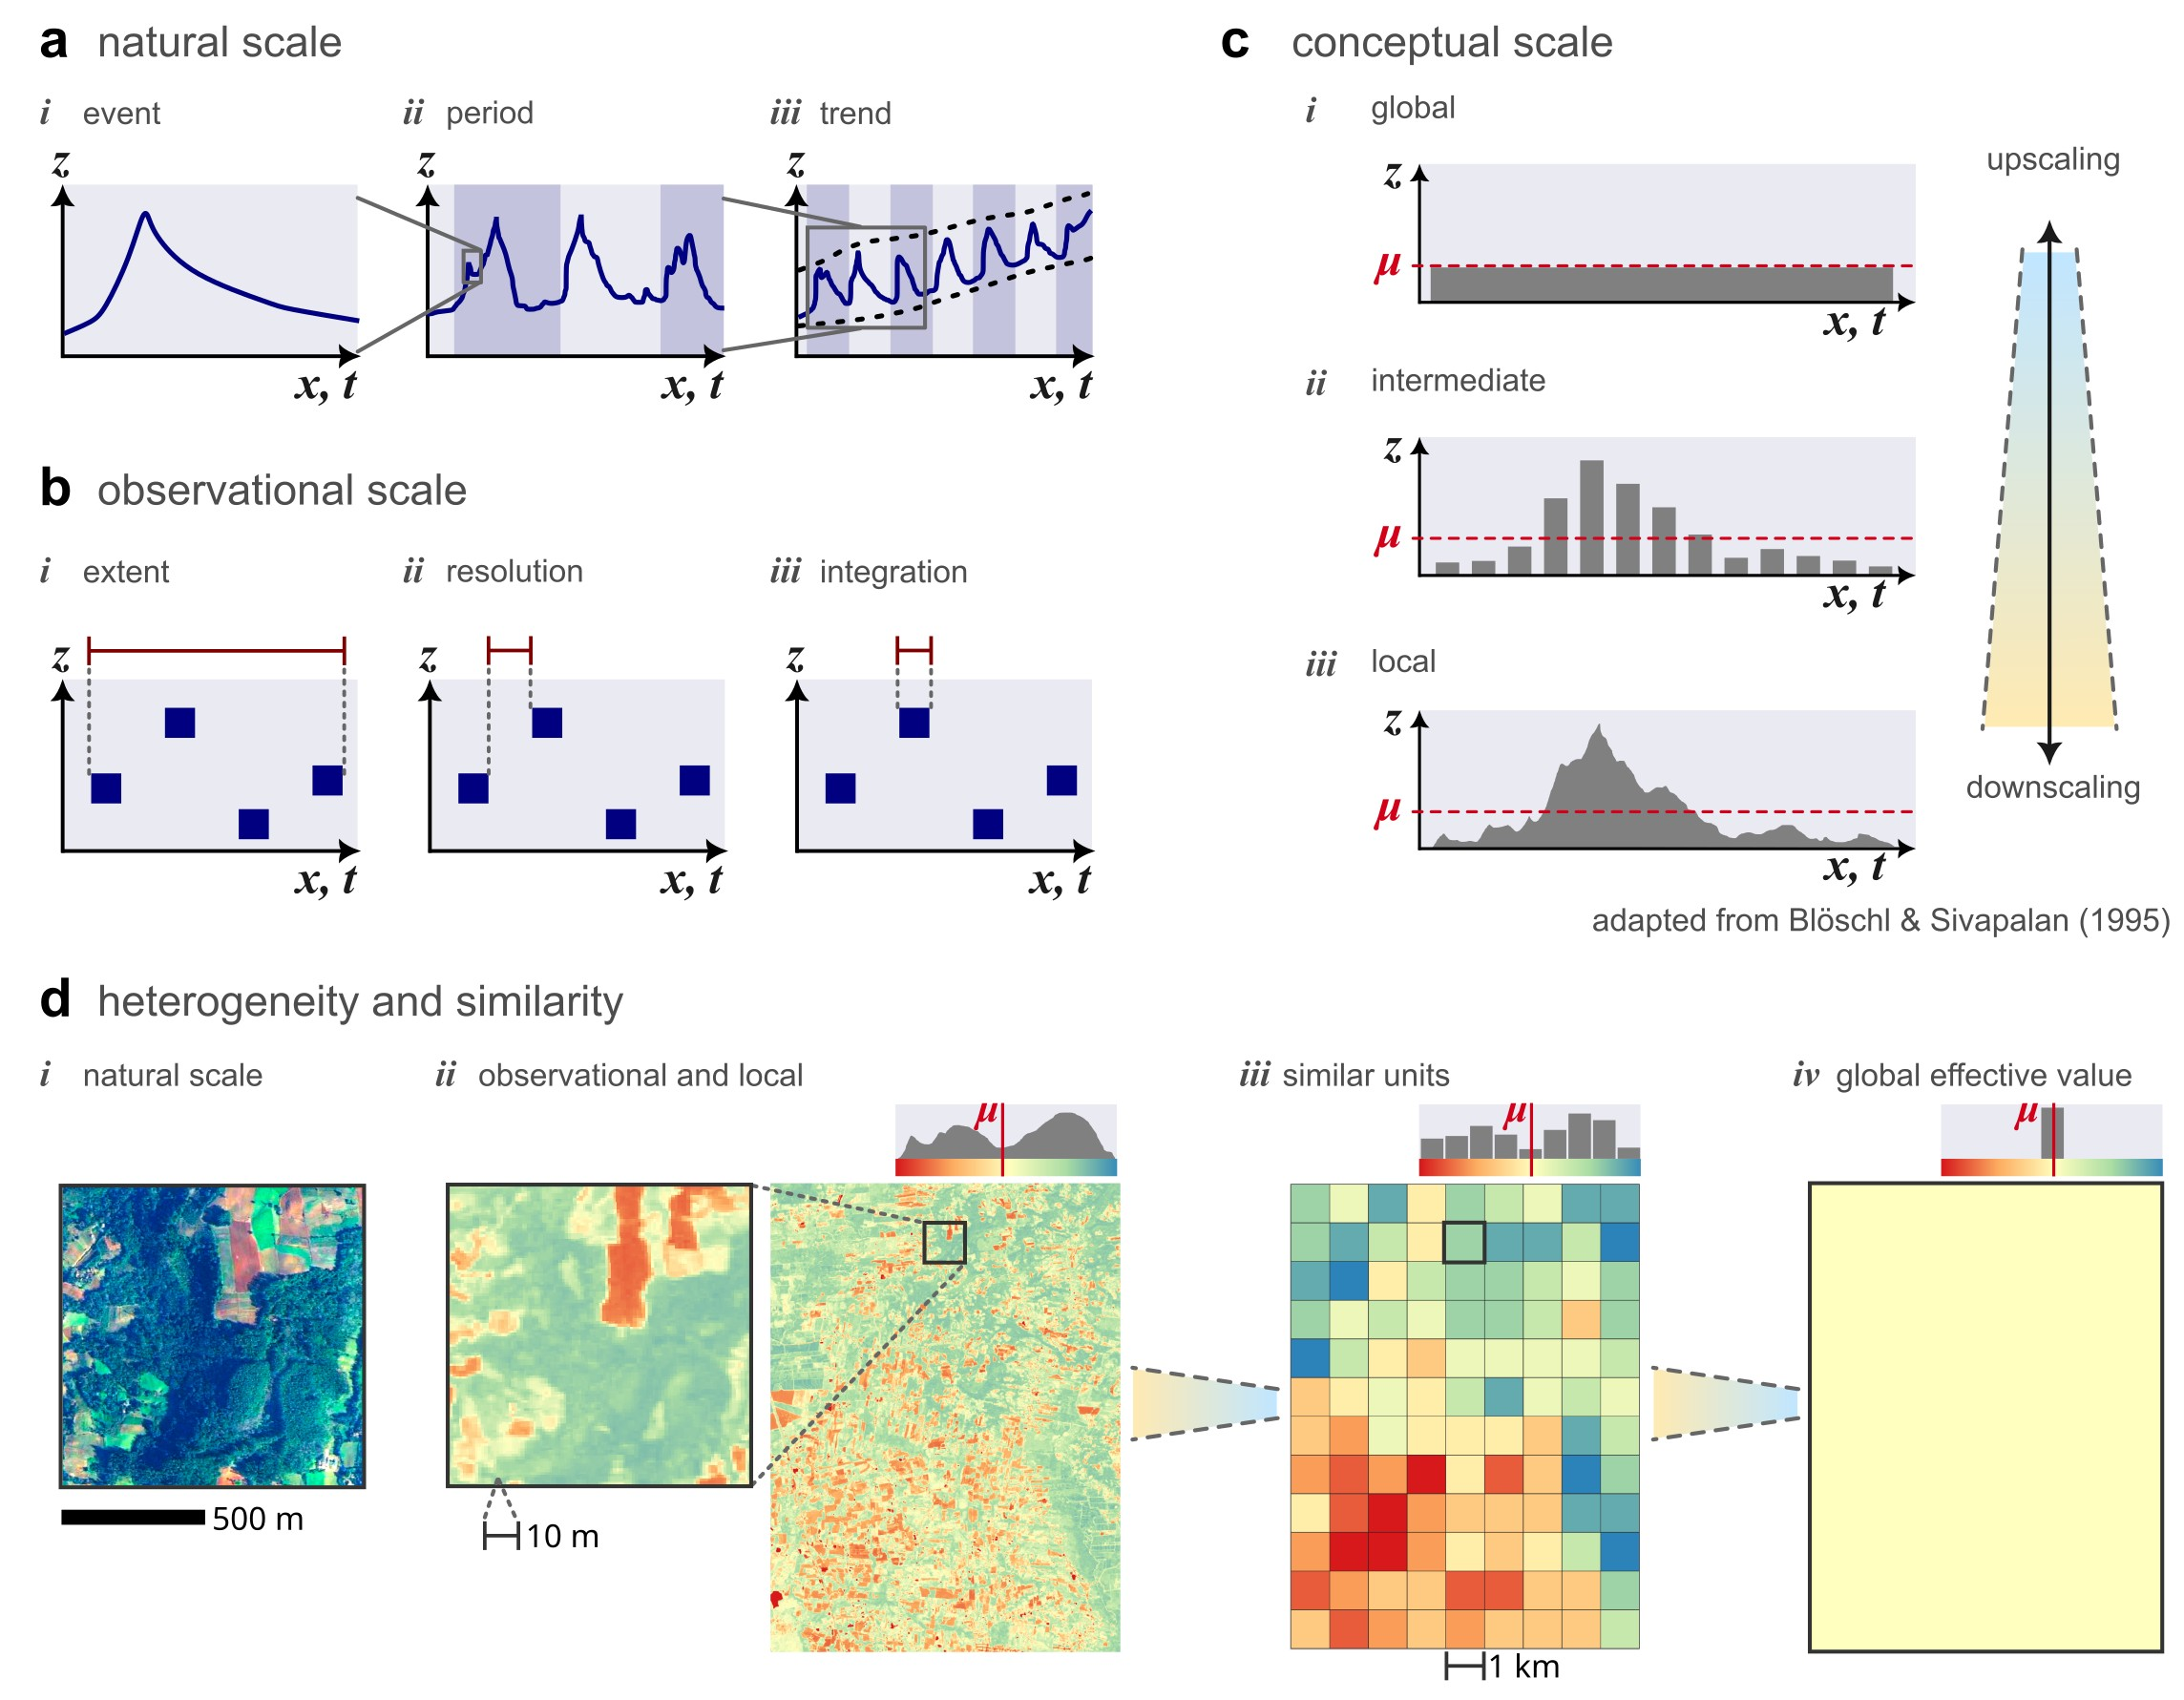
\includegraphics[width=0.98\linewidth]{figs/fig_scale_en.jpg}		
\caption[Schematic representation of different scales]
{\textbf{---\;Schematic representation of different scales.}
    Organized system by Blöschl \& Sivapalan (1995) \cite{Bloschl1995a} on the scales to be reconciled in time and space.\;\textbf{a}\;---\;The \gls{nat-scale} of processes varies in: (\textrm{\textit{i}}) event scale; (\textrm{\textit{ii}}) period scale, and; (\textrm{\textit{iii}}) trend scale.\;\textbf{b}\;---\;The \gls{obs-scale} presents three aspects: (\textrm{\textit{i}}) extent; (\textrm{\textit{ii}}) resolution, and; (\textrm{\textit{iii}}) integration.
    \;\textbf{c}\;---\;The \gls{model-scale} mediates between the \gls{nat-scale} and observational through \gls{scalab} methods. The \gls{model} operates at nested scales: (\textrm{\textit{i}}) \gls{glob-scale}; (\textrm{\textit{ii}}) intermediate scales, and; (\textrm{\textit{iii}}) \gls{loc-scale}.
    \;\textbf{d}\;---\;Effective values across scales: \gls{nat-scale}, where processes occur (\textrm{\textit{i}}); the \gls{obs-scale} establishes the lower limit of the local \gls{model-scale} (\textrm{\textit{ii}}); intermediate scale of similar units (\textrm{\textit{iii}}), and; effective process value at the \gls{glob-scale} (\textrm{\textit{iv}}).
}
\label{fig:hydro:scaling} 		
\end{figure}

\par Blöschl \& Sivapalan (1995) also advance to establish the crucial notion that there are three scales to be understood and reconciled in a modeling exercise: the \textbf{\gls{nat-scale}}, the \textbf{\gls{obs-scale}}, and the \textbf{\gls{model-scale}} (Figure \ref{fig:hydro:scaling}). The \gls{nat-scale} refers to the actual characteristic velocity exhibited by hydrological processes. It can be classified in different ways: as the lifespan of intermittent \textbf{events}, such as rises; by the \textbf{period} of annual events, such as snowmelt or the arrival of wet seasons; or by the duration of \textbf{trends} in long-duration stochastic processes, which exhibit some degree of autocorrelation, such as the depletion or filling of aquifers (Figure \ref{fig:hydro:scaling}\textbf{a}). The authors also expand this idea to spatial scales, defined by extent and trends in space, depending on the nature of the process. Some processes, like precipitation, do not have a preferred scale, as they distribute across multiple scales due to the nesting of subprocesses of both small and large scales, often with \textbf{spectral gaps} between them, that is, intervals where certain scales are less frequent. River runoff also follows this nested process structure, with flood peaks resulting from overlapping rapid response mechanisms and slower response mechanisms, such as groundwater or the occupation of large floodplains. Even rapid responses occur at different nested scales, such as flash rises from small soil plots and the formation of \gls{sat_areas} or \gls{nasc_efemeras}, manifesting at the slope scale. The \gls{obs-scale}, in turn, consists of the scale occupied by empirical evidence, arising from the need to manage a finite number of samples. It has three main aspects: the \textbf{extent} or coverage of the dataset, the \textbf{resolution} or spacing between samples, and the interval of \textbf{integration} of the sample (Figure \ref{fig:hydro:scaling}\textbf{b}). If sampling were infinite (or infinitesimal), the \gls{obs-scale} would coincide with the \gls{nat-scale}, capturing even the sample noise. In contrast, a very sparse sampling captures only the trend of the process, at best. A typical example of this is a rain gauge that, when read daily, reports the accumulated rainfall over a one-day interval, which may be much larger than the natural duration of a rain that occurred for only a few minutes. Nevertheless, this reading captures the trend of rainfall on a weekly or monthly scale. On the other hand, detailed soil samples can provide information about extremely localized hydraulic conductivity, which does not reflect the actual effect of macropores and preferential pathways at the slope scale. In this case, the process scale is broader, making point samples incomparable. Ideally, observations should be compatible with the scale of the processes of interest, positioning the sampling at an optimal point between the noise range and the trend range.

\par The \gls{nat-scale} and the \gls{obs-scale} relate in hydrological modeling by being mediated by the \gls{model-scale}, which is the scale of representation of the \gls{model} itself (Figure \ref{fig:hydro:scaling}\textbf{c}). Here lies the challenge of \gls{scalab}, as the \gls{model-scale} is often much larger or much smaller than the \gls{obs-scale}, introducing the inevitable \gls{error-commensu} $\varepsilon_{\Delta}$. As previously discussed, both the soil reservoir instantiated by \gls{sys-dyn} and an element of \gls{comp-grid} in a physically-based \gls{model} represent massive blocks that are incomparable with any point observation obtained in the field. Still, this error can be minimized by representing the \gls{sys-target} simultaneously at scales close to the available observations. In practice, this means dividing the \gls{model} into at least two nested levels: a more aggregated \textbf{\gls{glob-scale}} and a more detailed \textbf{\gls{loc-scale}}. Intermediate scales can also be incrementally instantiated, depending on the simulated hydrological processes and the available observations. At the \gls{glob-scale}, for example, the highly aggregated processes of the watershed are represented, such as river flow at a river section and the final flow of evapotranspiration, accumulated results of various subprocesses at smaller scales. At the \gls{loc-scale}, the details of these subprocesses are represented in small plots or mesh elements, such as rainfall input and runoff generation in different parts of the landscape. In this sense, the storage and flow variables, the \gls{parameters}, and the \gls{input-data} need to be compatible at all levels, necessitating the transfer of information from one level to another, that is, they need to be scaled.

\par The solution to this situation, therefore, consists of defining a \textbf{\gls{scaling-func}} that is valid between the simulated levels. These functions perform both \textbf{\gls{upscaling}}\footnote{Translation of \textit{upscaling} in English.} of information (bottom-up transfer) and \textbf{\gls{downscaling}}\footnote{Translation of \textit{downscaling} in English.} of information (top-down transfer). For material levels and flows, which are conserved, the \gls{upscaling} function can simply be the average or the sum over a given spatial or temporal extent. The global evapotranspiration flow of a watershed, therefore, would be the average of local flows (the integral). The \gls{downscaling}, on the other hand, generally consists of a non-trivial process that strongly depends on the process in question. In the case of soil and rock properties, such as hydraulic conductivity, the only way to unpack this information is through maps that reveal its pattern or \textbf{\gls{hetspatial}}. The same mapping strategy applies to \gls{parameters} related to vegetation or land cover, such as \gls{intercep-capacity} and \gls{sfmax}. In the absence of direct information, the use of \textbf{co-variables} or indicators can be employed with a \gls{downscaling} function, or \textbf{\gls{downscaling2}}, which adds new \gls{aux-hyp} to the theoretical framework of the \gls{model}. For example, Collischonn \textit{et al.} (2007) \cite{Collischonn2007} assume the \gls{hipotese} that the local \gls{intercep-capacity} is directly proportional to the Leaf Area Index (LAI), that is: $c_{\text{max}, i} = c \cdot \texttt{LAI}_{i}$, where $c$ is a proportionality constant. On the other hand, co-variables can be applied to \textit{group} spatial regions that theoretically exhibit \textbf{\gls{hydro-simi}}, that is, regions that are sufficiently homogeneous with respect to a given process at the assessed scale. In this context, the co-variable is referred to as the \textbf{hydrological similarity index}. The homogeneous regions resulting from this grouping, referred to as \textbf{\gls{urh}}, significantly reduce computational cost as they execute block processing, as opposed to the mesh processing required at the \gls{loc-scale}. Thus, models that apply this approach in \gls{downscaling} are regarded as \textbf{\gls{models-semid}}, as they do not represent the \gls{loc-scale} completely explicitly; the information is still compacted at the intermediate scale of the \gls{urh}. Finally, another challenge at the \gls{loc-scale} consists of the \textbf{\gls{regionalization}} of values located at points or patches to their lateral neighborhoods, at the same scale, as in the case of point rainfall observations that are interpolated to represent a continuous field in space. Just like in the case of \gls{downscaling2} of \gls{parameters}, this interpolation process introduces new \gls{aux-hyp} (and their uncertainties) into the modeling process.

\subsection{Scaling in \texttt{TOPMODEL}} \label{sec:hydro:topmodel}

\par An example of \gls{scalab} that is worth presenting at this moment is the \gls{model} \texttt{TOPMODEL}, initially articulated by Beven \& Kirkby (1979) in a study of the Crimple Beck basin (England, 8 km²) \cite{Beven1979a}. This \gls{model}, instantiated in the \gls{paradigma} of \gls{sys-dyn}, despite exhibiting a relatively simple compartment structure, effectively represents the mechanism of \gls{vsa}, producing rapid hydrological responses both through flash rises and through saturation excess in wet areas. During the simulation, the \gls{model} explicitly represents the expansion and contraction of \gls{sat_areas} along the terrain's thalweg as the watershed receives more or less rain. The flow of \gls{ground-rain} that directly impacts the saturated areas eventually becomes part of the rapid response of flood events, while the remaining portion of \gls{ground-rain} falls on dry soil and can then infiltrate.

% figure
\begin{figure}[t!] 
\centering				
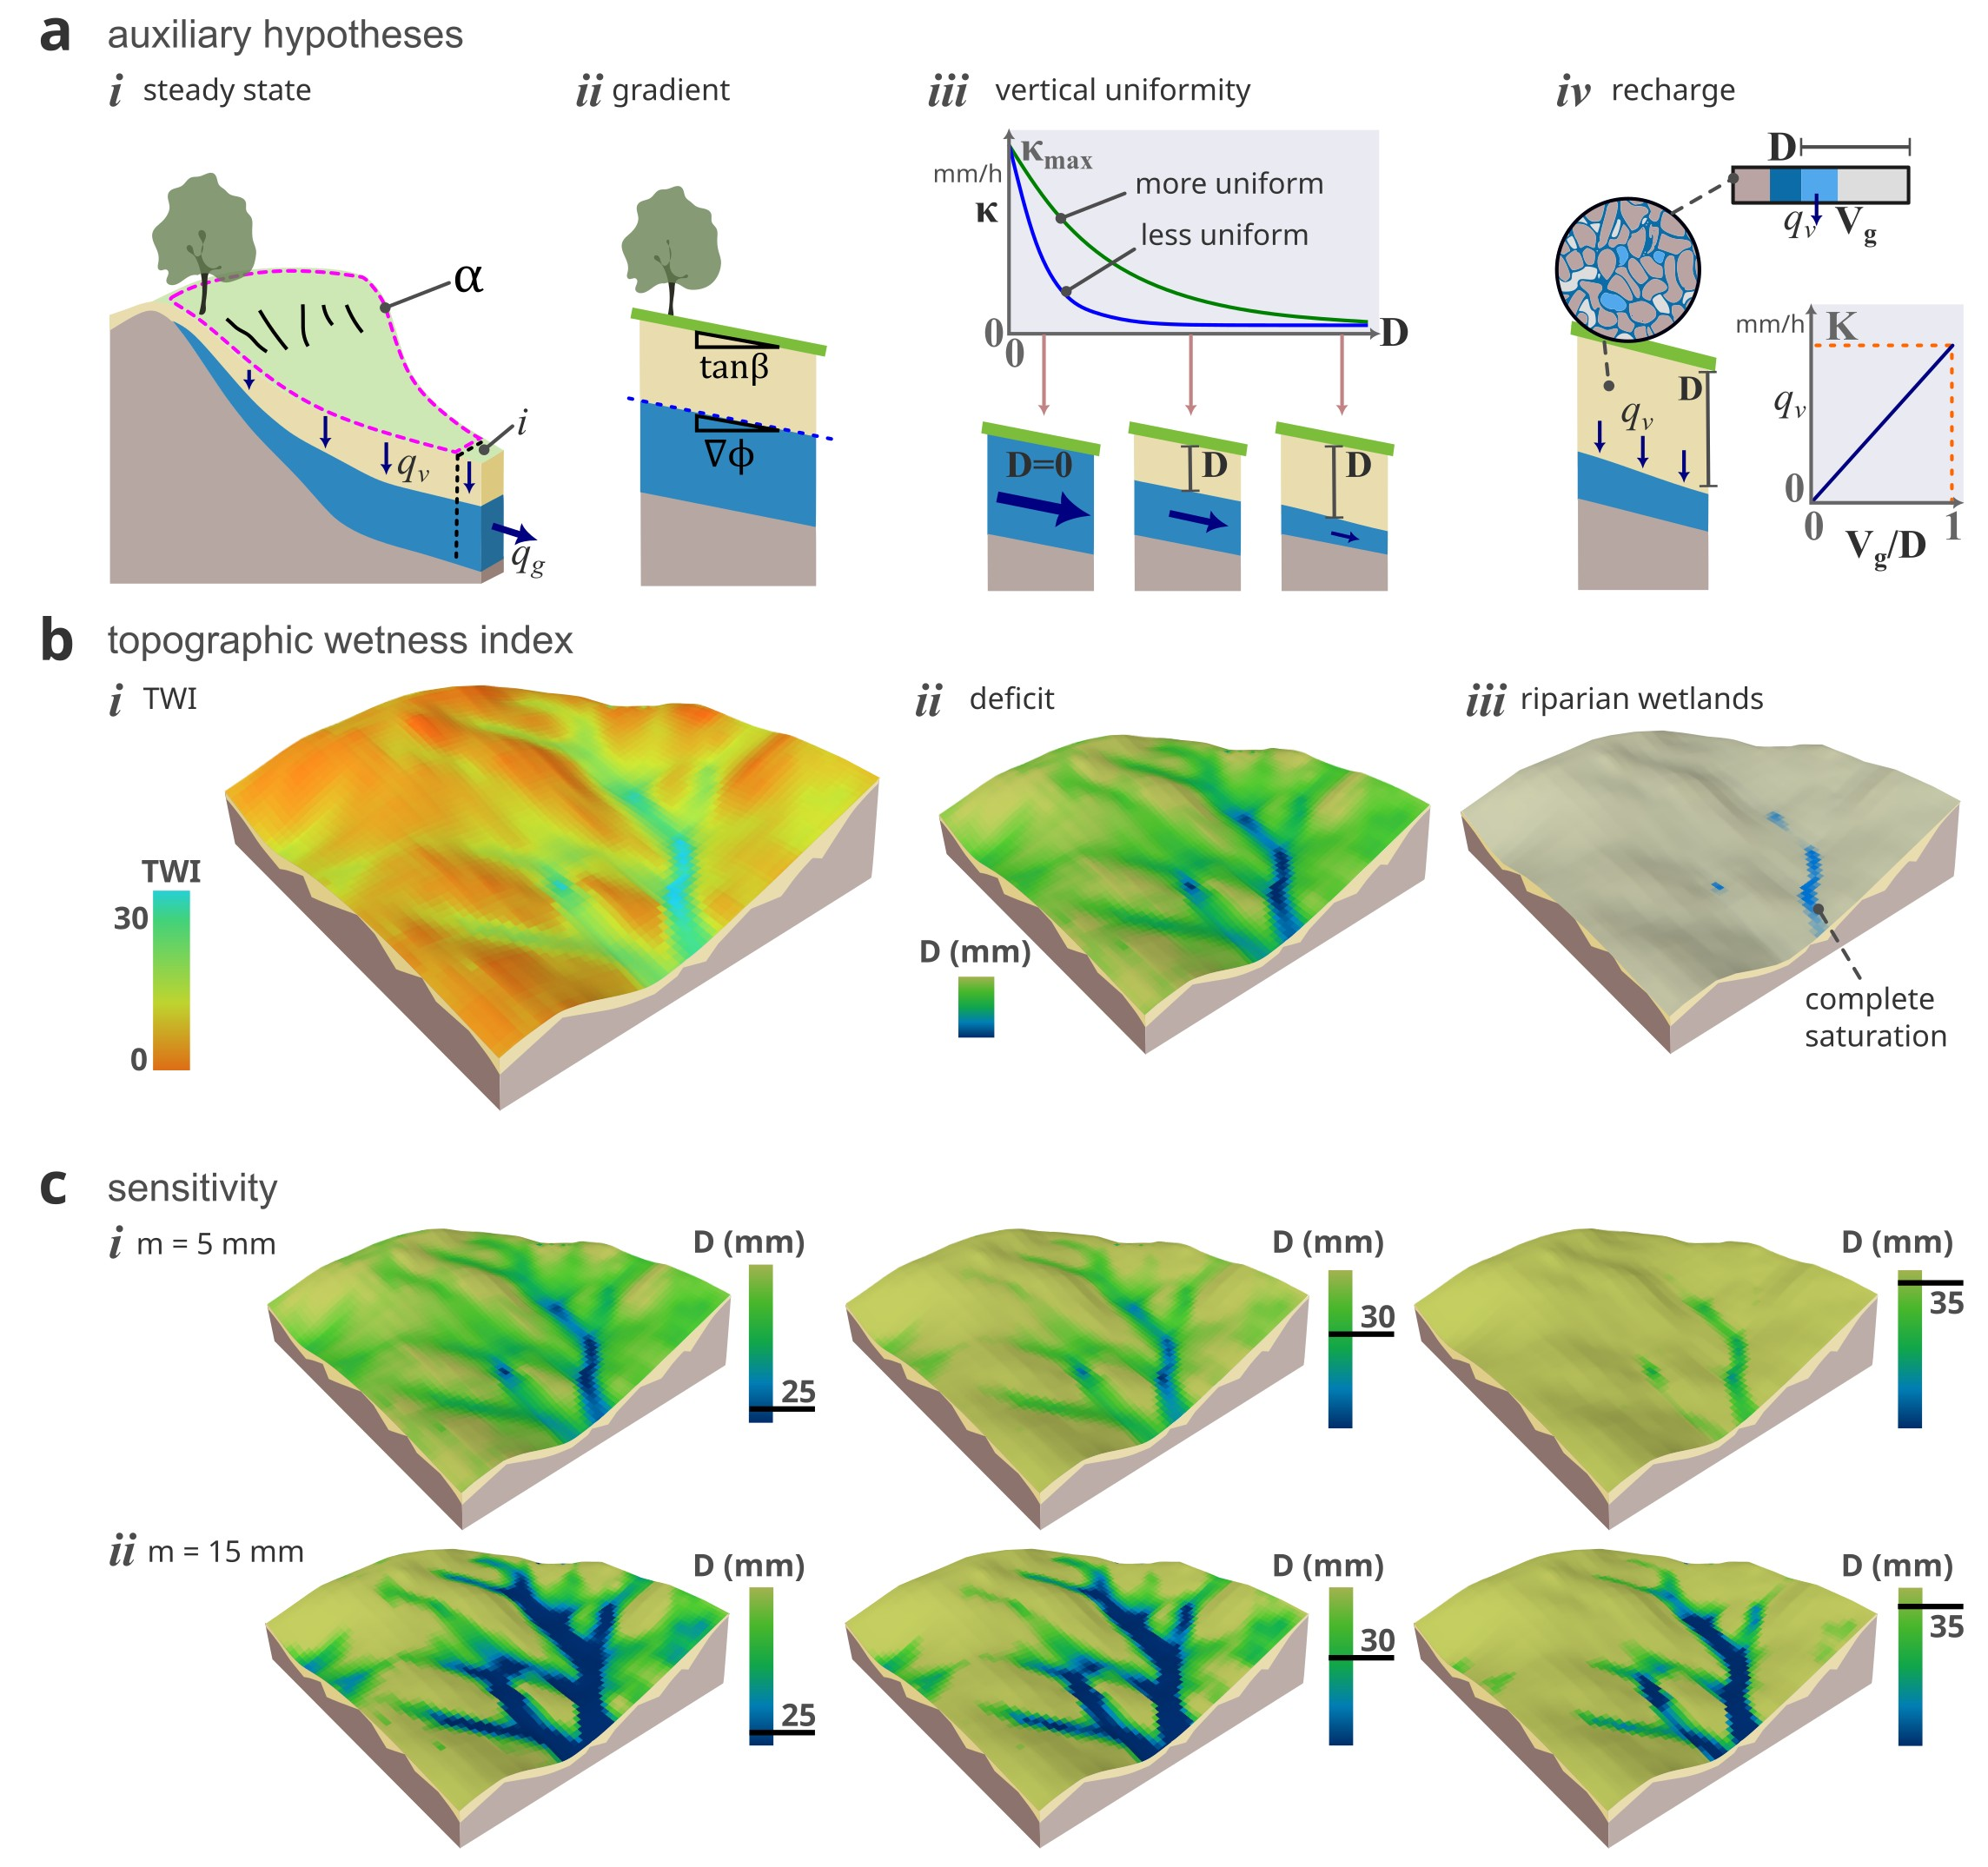
\includegraphics[width=0.98\linewidth]{figs/fig_topmodel_en.jpg}		
\caption[Hypotheses and implications of \texttt{TOPMODEL}]
{\textbf{---\;Hypotheses and implications of \texttt{TOPMODEL}.}
    The \texttt{TOPMODEL} is a \gls{model} that performs \gls{downscaling} of soil saturation from a topographic wetness index, the \gls{twi}.\;\textbf{a}\;---\;The classic version of the \texttt{TWI} in the \gls{model} is obtained by applying \gls{darcy-law} with three \gls{aux-hyp}: the \gls{hipotese} of steady-state (detail \textrm{\textit{i}}); the \gls{hipotese} of shallow soils (detail \textrm{\textit{ii}}), and; the \gls{hipotese} of vertical decay of transmissivity (detail \textrm{\textit{iii}}). A fourth auxiliary \gls{hipotese} is the flow of \gls{qv} as a linear function of the pressure in the \gls{unsat-zone} (detail \textrm{\textit{iv}}).\;\textbf{b}\;---\;The application of the \gls{scaling-func} of the \gls{model} uses the distribution of the \texttt{TWI} (detail \textrm{\textit{i}}) to determine the \gls{dgrav} and the \gls{sat_areas} at the \gls{loc-scale} (detail \textrm{\textit{ii}} and \textrm{\textit{iii}}).\;\textbf{c}\;---\; The details \textrm{\textit{i}} and \textrm{\textit{ii}} compare the sensitivity of local deficit distribution for more or less uniform soils (parameter $m$). A basin with more uniform soil ($m$ high) exhibits a more dispersed deficit distribution than a basin with less uniform soil ($m$ low). 
}
\label{fig:hydro:topmodel} 		
\end{figure}

\par Unlike the high computational cost of \gls{models-phys}, which need to numerically solve the Darcy-Richards Equation on a \gls{comp-grid}, the \texttt{TOPMODEL} approach identifies the spatial pattern of soil saturation at the \gls{loc-scale} through a low-cost computational \gls{downscaling} function (distribution). In the presence of empirical evidence solely from rainfall and discharge, both approaches are empirically equivalent, with the advantage that \texttt{TOPMODEL} is simpler (i.e., it has a greater degree of falsifiability). In this sense, the use of a physically-based \gls{model} becomes justified only when more detailed evidence becomes available, such as piezometric levels, \gls{bedrock_topo}, and water quality \gls{parameters}\footnote{For detailed mappings of contamination plume evolution in the subsurface, for example, a physically-based \gls{model} is the only alternative that offers the ontology compatible with the problem at hand.}.

\par Soil saturation in \texttt{TOPMODEL} is expressed by the \gls{dgrav} at the \gls{loc-scale} in the watershed, denoted by $D_{i} \; [\text{L}]$, where $i$ is any element of a mesh that divides the basin into $N$ elements. That is, when $D_{i} = 0$, the soil is completely saturated in element $i$, and the water from the \gls{ground-rain} that falls on this element cannot infiltrate, remaining accumulated on the surface until it reaches the \gls{sfmax}. The compaction function of this variable transfers information across scales through the simple calculation of the average:
\begin{linenomath*}
\begin{equation}
\label{eq:topmodel:d1}
D = \frac{1}{N} \sum^{N}_{i} D_{i} \quad  \forall \; i \in \{ 1, 2, ..., N\}
\end{equation}
\end{linenomath*}
Where $D \; [\text{L}]$ is the global deficit and; $D_{i} \; [\text{L}]$ is the local deficit. Thus, the \gls{dgrav} at the \gls{glob-scale} consists of the average of the deficits at the \gls{loc-scale} $D_{i}$. The distribution of gravitational deficit from \gls{glob-scale} to \gls{loc-scale}, on the other hand, is based on the use of a \textbf{\gls{tsi}}. This index is thus considered a \textit{co-variable} of the gravitational deficit, such that the \textit{deviations from the mean} between the \gls{loc-scale} and global are linearly proportional:
\begin{linenomath*}
\begin{equation}
\label{eq:topmodel:d2}
D - D_{i}  \propto \lambda_{i} - \lambda  \quad \forall \; i
\end{equation}
\end{linenomath*}
Where $\lambda_{i}\; [-]$ is the \gls{tsi} at the \gls{loc-scale}, and; $\lambda \; [-]$ is the \gls{tsi} at the \gls{glob-scale}, that is, the average obtained by:
\begin{linenomath*}
\begin{equation}
\label{eq:topmodel:d3}
\lambda = \frac{1}{N} \sum^{N}_{i} \lambda_{i} \quad  \forall \; i 
\end{equation}
\end{linenomath*}
The Equation \eqref{eq:topmodel:d2} becomes an equality when a proportionality constant is introduced:
\begin{linenomath*}
\begin{equation}
\label{eq:topmodel:d4}
D - D_{i}  = \omega (\lambda_{i} - \lambda ) \quad \forall \; i
\end{equation}
\end{linenomath*}
Where $\omega \; [\text{L}]$ is the \gls{scalab} factor. By rearranging the terms, the local gravitational deficit $D_{i}$ is obtained through the following \gls{downscaling2}:
\begin{linenomath*}
\begin{equation}
\label{eq:topmodel:d5}
D_{i}  = D + \omega (\lambda - \lambda_{i}) \quad \forall \; i
\end{equation}
\end{linenomath*}
Where $D_i$ must be truncated at zero, so as not to take negative values. In a hydrological \gls{model}, Equation \eqref{eq:topmodel:d5} aims to locally distribute the global deficit $D$ at each time step, allowing other variables at the \gls{loc-scale} to be specified, such as \gls{qv} and surface runoff. In this case, the elements $i$ where $D_i = 0$ correspond precisely to saturated soil areas, the \gls{vsa} that will invariably produce rapid runoff responses in the face of rainfall events.

\par Here, it is worth noting that Equation \eqref{eq:topmodel:d5} is a generically applicable formulation for any \gls{tsi} $\lambda_{i}$. However, Beven \& Kirkby (1979) originally deduced it theoretically from \gls{darcy-law} and some \gls{aux-hyp} (see Figure \ref{fig:hydro:topmodel}\textbf{a}), resulting in the \gls{tsi} $\lambda_{i}$ then referred to as \textbf{\gls{twi}}, which is calculated by:
\begin{linenomath*}
\begin{equation}
\label{eq:topmodel:twi}
\text{T}_{i}  = \ln{(\alpha_{i}/\tan \beta_{i})} \quad \forall \; i
\end{equation}
\end{linenomath*}
Where $\alpha_{i}\; [L^{2}L^{-1}]$ is the local drainage area per unit of contour, and; $\beta_{i} [-]$ is the local slope of the terrain. That is, the local potential for soil saturation (1) is greater the larger the drainage area, and (2) is greater the smaller the slope of the terrain. Maps of \acrshort{atwi} can thus be obtained directly from a \textbf{\gls{dem}} using geoprocessing techniques. The local slope $\beta_{i}$, for example, can be estimated using Horn's method (1981) \cite{Horn1981a} by computing the altitude differences in the west-east and north-south directions in the \textbf{mantissa}\footnote{In a rectangular mesh of elements, the mantissa consists of the eight neighboring elements surrounding any given element.} of the mesh element. On the other hand, determining the local drainage area per unit of contour $\alpha_{i}$ requires a more computationally intensive analysis, as it is necessary to trace all upstream mesh elements for each given element. This cannot occur before removing spurious depressions in the \acrshort{adem}, which cause the method to truncate. Barnes \textit{et al.} (2014) \cite{Barnes2014a} introduce an efficient algorithm for this process, as well as review various other strategies available in the literature. Once a depression-free \acrshort{adem} is obtained, the drainage area is computed using flow accumulation methods, such as the unidirectional flow method by O'Callaghan \& Mark (1984) \cite{Ocallaghan1984a} or the multidirectional flow method by Freeman (1991) \cite{Freeman1991a}. Quinn \textit{et al.} (1991) \cite{Quinn1991b} demonstrate that there is substantial sensitivity in \texttt{TOPMODEL} regarding the choice of flow accumulation method, suggesting that the multidirectional method presents better empirical adequacy. Additionally, the authors also evaluate the possibility of \textit{overlapping} methods to adjust the \acrshort{atwi} between ephemeral (multidirectional) and perennial (unidirectional) drainage regions.

\par There are three \gls{aux-hyp} that theoretically underpin Equation \eqref{eq:topmodel:twi}. The first is the \gls{hipotese} of steady-state (detail \textit{i} in Figure \ref{fig:hydro:topmodel}\textbf{a}), which establishes that a local steady-state condition is achieved at each time step, such that the lateral base flow equals the recharge flow:
\begin{linenomath*}
\begin{equation}
\label{eq:topmodel:prem1}
q_{\text{g}, i} = q_{\text{v}} \cdot \alpha_{i}  \quad \, \forall i
\end{equation}
\end{linenomath*}
Where $q_{\text{g}, i}\; [L^{2}T^{-1}]$ is the lateral base flow per unit of contour; $q_{\text{v}}\; [LT^{-1}]$ is the recharge flow, and; $\alpha_{i}\; [L^{2}L^{-1}]$ is the local drainage area per unit of contour. The second auxiliary \gls{hipotese} (detail \textit{ii} in Figure \ref{fig:hydro:topmodel}\textbf{a}) assumes that the soil is shallow enough for the local hydraulic gradient in the water table $\nabla \Phi_{i}\; [LL^{-1}]$ to be approximated by the local slope of the terrain $\tan \beta_{i}\; [LL^{-1}]$:
\begin{linenomath*}
\begin{equation}
\label{eq:topmodel:prem2}
\nabla \Phi_{i} = \tan \beta_{i} \quad \, \forall i
\end{equation}
\end{linenomath*}
The third auxiliary \gls{hipotese} (detail \textit{iii} in Figure \ref{fig:hydro:topmodel}\textbf{a}) is that local hydraulic conductivity $K_{ i}\; [LT^{-1}]$ decays exponentially with gravitational deficit, meaning that the drier the soil, the lower the hydraulic conductivity. This is a \gls{hipotese} consistent with empirical observations that the upper soil horizons, with organic layers and macropores, exhibit higher conductivity than the lower, more mineral parts. The hydraulic conductivity per unit of contour is expressed as \textbf{\gls{trans-hyd}}, leading to the \gls{hipotese} taking the following form:
\begin{linenomath*}
\begin{equation}
\label{eq:topmodel:prem3}
\kappa_{i} = \kappa_{\text{max}} \cdot e^{-D_{i}/m}  \quad \, \forall i
\end{equation}
\end{linenomath*}
Where $\kappa_{i}\; [L^{2}T^{-1}]$ is the local transmissivity; $\kappa_{\text{max}}\; [L^{2}T^{-1}]$ is the maximum transmissivity under saturated conditions; $D_{i}\; [L]$ is the local deficit, and; $m\; [L]$ is the constant of \textbf{vertical uniformity of the soil}. The larger the value of $m$, the more gradual the change in transmissivity as a function of saturation, such that: $\lim_{m\to\infty} T = T_{\text{max}}$. Considering the flows per unit of contour of the terrain, Darcy's Equation \eqref{eq:darcy-5} takes the following structure:
\begin{linenomath*}
\begin{equation}
\label{eq:topmodel:darcy1}
u = K \nabla \Phi \Rightarrow q_{\text{g,i}} = \kappa_{\text{max}} \nabla \Phi_{i} \quad \, \forall i
\end{equation}
\end{linenomath*}
Where the Darcy velocity $u \; [LT^{-1}]$ corresponds to the lateral base flow per unit of contour $q_{\text{g}, i}\; [L^{2}T^{-1}]$. Connecting Equations \eqref{eq:topmodel:prem1}, \eqref{eq:topmodel:prem2}, and \eqref{eq:topmodel:prem3} in Darcy's Equation \eqref{eq:topmodel:darcy1}:
\begin{linenomath*}
\begin{equation}
\label{eq:topmodel:darcy2}
q_{\text{v}} \alpha_{i} = \kappa_{\text{max}} e^{-D_{i}/m} \tan \beta  \quad \, \forall i
\end{equation}
\end{linenomath*}
The local deficit $D_i$ can be isolated, yielding:
\begin{linenomath*}
\begin{equation}
\label{eq:topmodel:darcy3}
D_{i} = -m \ln{(q_{\text{v}} \alpha_{i} /\kappa_{\text{max}}\tan \beta_{i})}  \quad \, \forall i
\end{equation}
\end{linenomath*}
By logarithmic properties, the following relationship is also obtained, isolating the terms of static hydrological variables from dynamic hydrological variables and purely topographic terms:
\begin{linenomath*}
\begin{equation}
\label{eq:topmodel:plug1}
\ln(q_{\text{v}}/\kappa_{\text{max}}) = - D_{i}/m - \ln(\alpha_{i} / \tan \beta_{i})  \quad \, \forall i
\end{equation}
\end{linenomath*}
Now, considering that the global deficit $D$ is the average of the local deficits $D_i$, Equation \eqref{eq:topmodel:darcy3} can be applied in Equation \eqref{eq:topmodel:d1}:
\begin{linenomath*}
\begin{equation}
\label{eq:topmodel:d6}
D = \frac{1}{N} \sum^{N}_{i} -m \ln{(q_{\text{v}} \alpha_{i} /\kappa_{\text{max}}\tan \beta_{i})} \quad  \forall \; i 
\end{equation}
\end{linenomath*}
Using summation properties and assuming $m$ and $\kappa_{\text{max}}$ are spatially homogeneous, local terms can be isolated from global terms:
\begin{linenomath*}
\begin{equation}
\label{eq:topmodel:d7}
D = \left[ -m\frac{1}{N} \sum^{N}_{i} \ln{(\alpha_{i}/\tan \beta_{i})}\right]  - \left[m \ln{(q_{\text{v}} /\kappa_{\text{max}})}\right] \quad  \forall \; i 
\end{equation}
\end{linenomath*}
Substituting \eqref{eq:topmodel:plug1} into \eqref{eq:topmodel:d7}, we arrive at:
\begin{linenomath*}
\begin{equation}
\label{eq:topmodel:d8}
D = \left[ -m\frac{1}{N} \sum^{N}_{i} \ln{(\alpha_{i}/\tan \beta_{i})}\right] + D_{i} + m \ln{(\alpha_{i}/\tan \beta_{i})} \quad  \forall \; i 
\end{equation}
\end{linenomath*}
Which is homologous to Equation \eqref{eq:topmodel:d4}, with $\lambda_{i} = \text{T}_{i}$ and $\omega = m$:
\begin{linenomath*}
\begin{equation}
\label{eq:topmodel:d9}
D_{i}= D +   m  \left[ \left( \frac{1}{N} \sum^{N}_{i} \text{T}_{i}\right) - \text{T}_{i}\right] \quad  \forall \; i 
\end{equation}
\end{linenomath*}

\par In total, the version of \texttt{TOPMODEL} articulated by Beven \& Kirkby (1979) includes seven \gls{parameters} regulating reservoirs and flows of the water balance in the soil, as well as a flow velocity parameter used in simulating the propagation of flow in the drainage network of channels. In particular, the \gls{parameters} $m$ and $Q_{\text{g},\text{max}}$ can be estimated \textit{a priori} from the \gls{deple-curve} of the river during observed recessions in cold weather (with low water loss due to evapotranspiration), as the integration of Equation \eqref{eq:topmodel:prem3} over all lateral stretches of channels determines the base flow:
\begin{linenomath*}
\begin{equation}
\label{eq:topmodel:prem3a}
Q_{\text{g}, t} = Q_{\text{g},\text{max}} \cdot e^{-D_{t}/m}  \quad \forall \; t
\end{equation}
\end{linenomath*}
Where $Q_{\text{g}}\;[L^{3}T^{-1}]$ is the base flow; $Q_{\text{g},\text{max}}\;[L^{3}T^{-1}]$ is the production capacity of the aquifer; $D_t\;[\text{L}]$ is the global deficit at time $t$, and; $m\; [L]$ is the vertical uniformity of the soil. The details in Figure \ref{fig:hydro:topmodel}\textbf{b} demonstrate how sensitive the \gls{model} is to changes in the vertical uniformity of the soil. The distribution of local deficit, in this regard, becomes increasingly more dispersed as the value of $m$ increases. This occurs evidently because it acts as a multiplier in the \gls{scaling-func} (Equation \eqref{eq:topmodel:d5}). The practical implication is that a basin with relatively more uniform soil will produce relatively more \gls{sat_areas}. The physical interpretation of this implication is that, keeping the same production capacity of the aquifer $Q_{\text{g},\text{max}}$, a more uniform soil transmits more water, draining the higher slopes more quickly as the global deficit of the basin increases.

\par The \gls{cond-hyd} of the soil is employed in \texttt{TOPMODEL} in a revision of the \gls{model} presented by Beven \& Wood (1983) \cite{Beven1983a}, under a fourth \gls{aux-hyp} concerning the flow of \gls{qv} (detail \textit{iv} in Figure \ref{fig:hydro:topmodel}\textbf{a}). In this case, the authors assume that the vertical flow of \gls{qv} at the \gls{loc-scale} tends linearly toward the value of \gls{cond-hyd} as the \gls{unsat-zone} becomes pressurized by hydraulic load\footnote{In fact, the authors introduced a peculiar term of \textit{delay per unit deficit} $t_d\; [TL^{-1}]$, causing the recharge equation to take the following form: $q_v = V_g / t_d D$. Although identical, this notation does not make much hydrological sense, especially considering that hydraulic conductivity is a well-established concept. In observance of John Sterman's modeling principles (Chapter 2), I maintained a clearer notation.}:
\begin{linenomath*}
\begin{equation}
\label{eq:topmodel:qv}
q_{\text{v}, i} = K \cdot \frac{V_{\text{g}, i}}{D_i}  \quad \forall \; i
\end{equation}
\end{linenomath*}
Where $q_{\text{v}, i}\;[LT^{-1}]$ is the local recharge; $K\;[LT^{-1}]$ is the hydraulic conductivity of the soil; $V_{\text{g}, i}\;[L]$ is the local gravitational water in the \gls{unsat-zone}, and; $D_{i} \; [\text{L}]$ is the local deficit. That is, the pressurization in the \gls{unsat-zone} is represented by the ratio of gravitational water to the saturation deficit, which can also be interpreted as the \textit{capacity} for storing gravitational water in the \gls{unsat-zone}. Thus, as the gravitational water in the \gls{unsat-zone} is constrained by the deficit, the ratio $V_{\text{g}, i}/D_i$ tends to 1 when the deficit approaches zero, or $\lim _{D_i \to 0} q_v= K$.

\par The classic version of \texttt{TOPMODEL} is essentially summarized by the concepts and equations organized above, with its main \gls{hipotese} being the \gls{downscaling} function represented by Equation \eqref{eq:topmodel:d5}. Its fundamental hallmark, therefore, is to represent rises produced both by overland runoff and by saturation excess, which is accomplished with simulated maps of \gls{sat_areas} obtained from a topographic indicator (in this case, the \texttt{TWI}). On the other hand, the other flow equations, such as the evapotranspiration flow in each reservoir of the \gls{system} and hydraulic propagation downstream, are couplings to the basic \gls{model} that can be modified or not. Authors like Ambroise \textit{et al.} (1996) \cite{Ambroise1996a} and Iorgulescu \& Musy (1997) \cite{Iorgulescu1997a} have indeed implemented generalizations in the \gls{aux-hyp}, deriving generic formulations to calculate the topographic wetness index. In the same vein, Beven \& Freer (2001) \cite{Beven2001b} produced a more complex version of the \gls{model}, called Dynamic \texttt{TOPMODEL}, where the local drainage area $\alpha_i$ is replaced by the local recharge area $\alpha_{v, i}$, which needs to be updated at each time step of the simulation (a procedure that makes this version computationally more intensive).

\par Besides the capacity for modifications, Beven \cite{Beven2012} suggests that the classic version can be instantiated as a semi-distributed \gls{model}, aggregating the mean of the \gls{tsi} into discrete ranges of its histogram in \gls{urh}. That is, in small incremental ranges of the index, it is assumed that the mesh elements exhibit \gls{hydro-simi}. This way, relatively broad regions of elements in space are scaled to a relatively small number of homogeneous blocks, drastically reducing the computational cost of simulating the \gls{model}. More detailed maps at the \gls{loc-scale} can thus be recovered after processing—one just needs to use the source map of the \gls{tsi} to position the simulated processes in their respective mesh elements. Although it is a practically oriented strategy related to the \gls{proced-model}, using a semi-distributed \gls{model} has implications for the simulated results. For instance, mesh processing in a fully distributed approach allows for the representation of spatial and temporal \gls{hetspatial} of other flows and \gls{parameters} (such as rainfall distribution, for example), which is not possible in a semi-distributed approach. Since the intensive use of simulations in diagnostic techniques requires that the simulation time of the models not be a critical bottleneck (see Section \ref{sec:sys:diags}), these issues must be weighed to arrive at an appropriate strategy for addressing the \gls{problem-dimens}.

\subsection{Scaling in \texttt{PLANS}} \label{sec:hydro:plans}

\par The \gls{model} \texttt{PLANS} is a version of \texttt{TOPMODEL} that exhibits strategies for both the generalization of the \gls{tsi} and semi-distributed modeling. Illustrated in Figure \ref{fig:hydro:plans}, the \gls{model} was developed by myself and colleagues with the explicit purpose of establishing a tool to assist in the formulation of \gls{ebp} in the context of expanding \acrfull{nbs}\footnote{The acronym \texttt{PLANS} stands for \textit{Planning Nature-based Solutions}, meaning \say{Planning Nature-Based Solutions}. The overarching goal of the initiative is to establish a toolkit of concepts and tools to address the challenges of expanding \acrshort{nbs}. The \gls{model} presented here might be designated as the hydrological module of the \texttt{PLANS} project.} in watersheds in Brazil \cite{Possantti2022a, Possantti2023a}. The term \say{\acrlong{nbs}} serves as a conceptual umbrella for a collection of techniques and approaches at different scales that draw inspiration from or utilize natural processes. We will see later, in the next chapter, that this public policy movement can benefit from the use of modeling within a framework of basic principles. The first version of the \gls{model} \texttt{PLANS} was a somewhat more complex \gls{model} than the prototype presented in the previous chapter. This initial version was used in an exploratory modeling study that applied search techniques to optimally allocate the expansion of \acrshort{nbs} over time under future scenarios \cite{Possantti2022a}. On one hand, the application of the \gls{model} successfully highlighted nuances and stimulated revisions of \gls{mental-models}. In this case, the \gls{model} found that the expansion of the listed \acrshort{nbs} yields scaling benefits in relatively more degraded watersheds—the incremental performance in more preserved areas likely does not justify the investment. On the other hand, the highly aggregated nature of this initial version did not allow for an exact assessment of \textit{where} the expansion of \acrshort{nbs} should occur, causing the \gls{model} to fail in addressing the spatial allocation problem. This shortcoming forced me to abandon the initial structure and instead instantiate a version of \texttt{TOPMODEL} tailored to address the issue of expanding \acrshort{nbs} both in time and space \cite{Possantti2023a}.

% figure
\begin{figure}[t!] 
\centering				
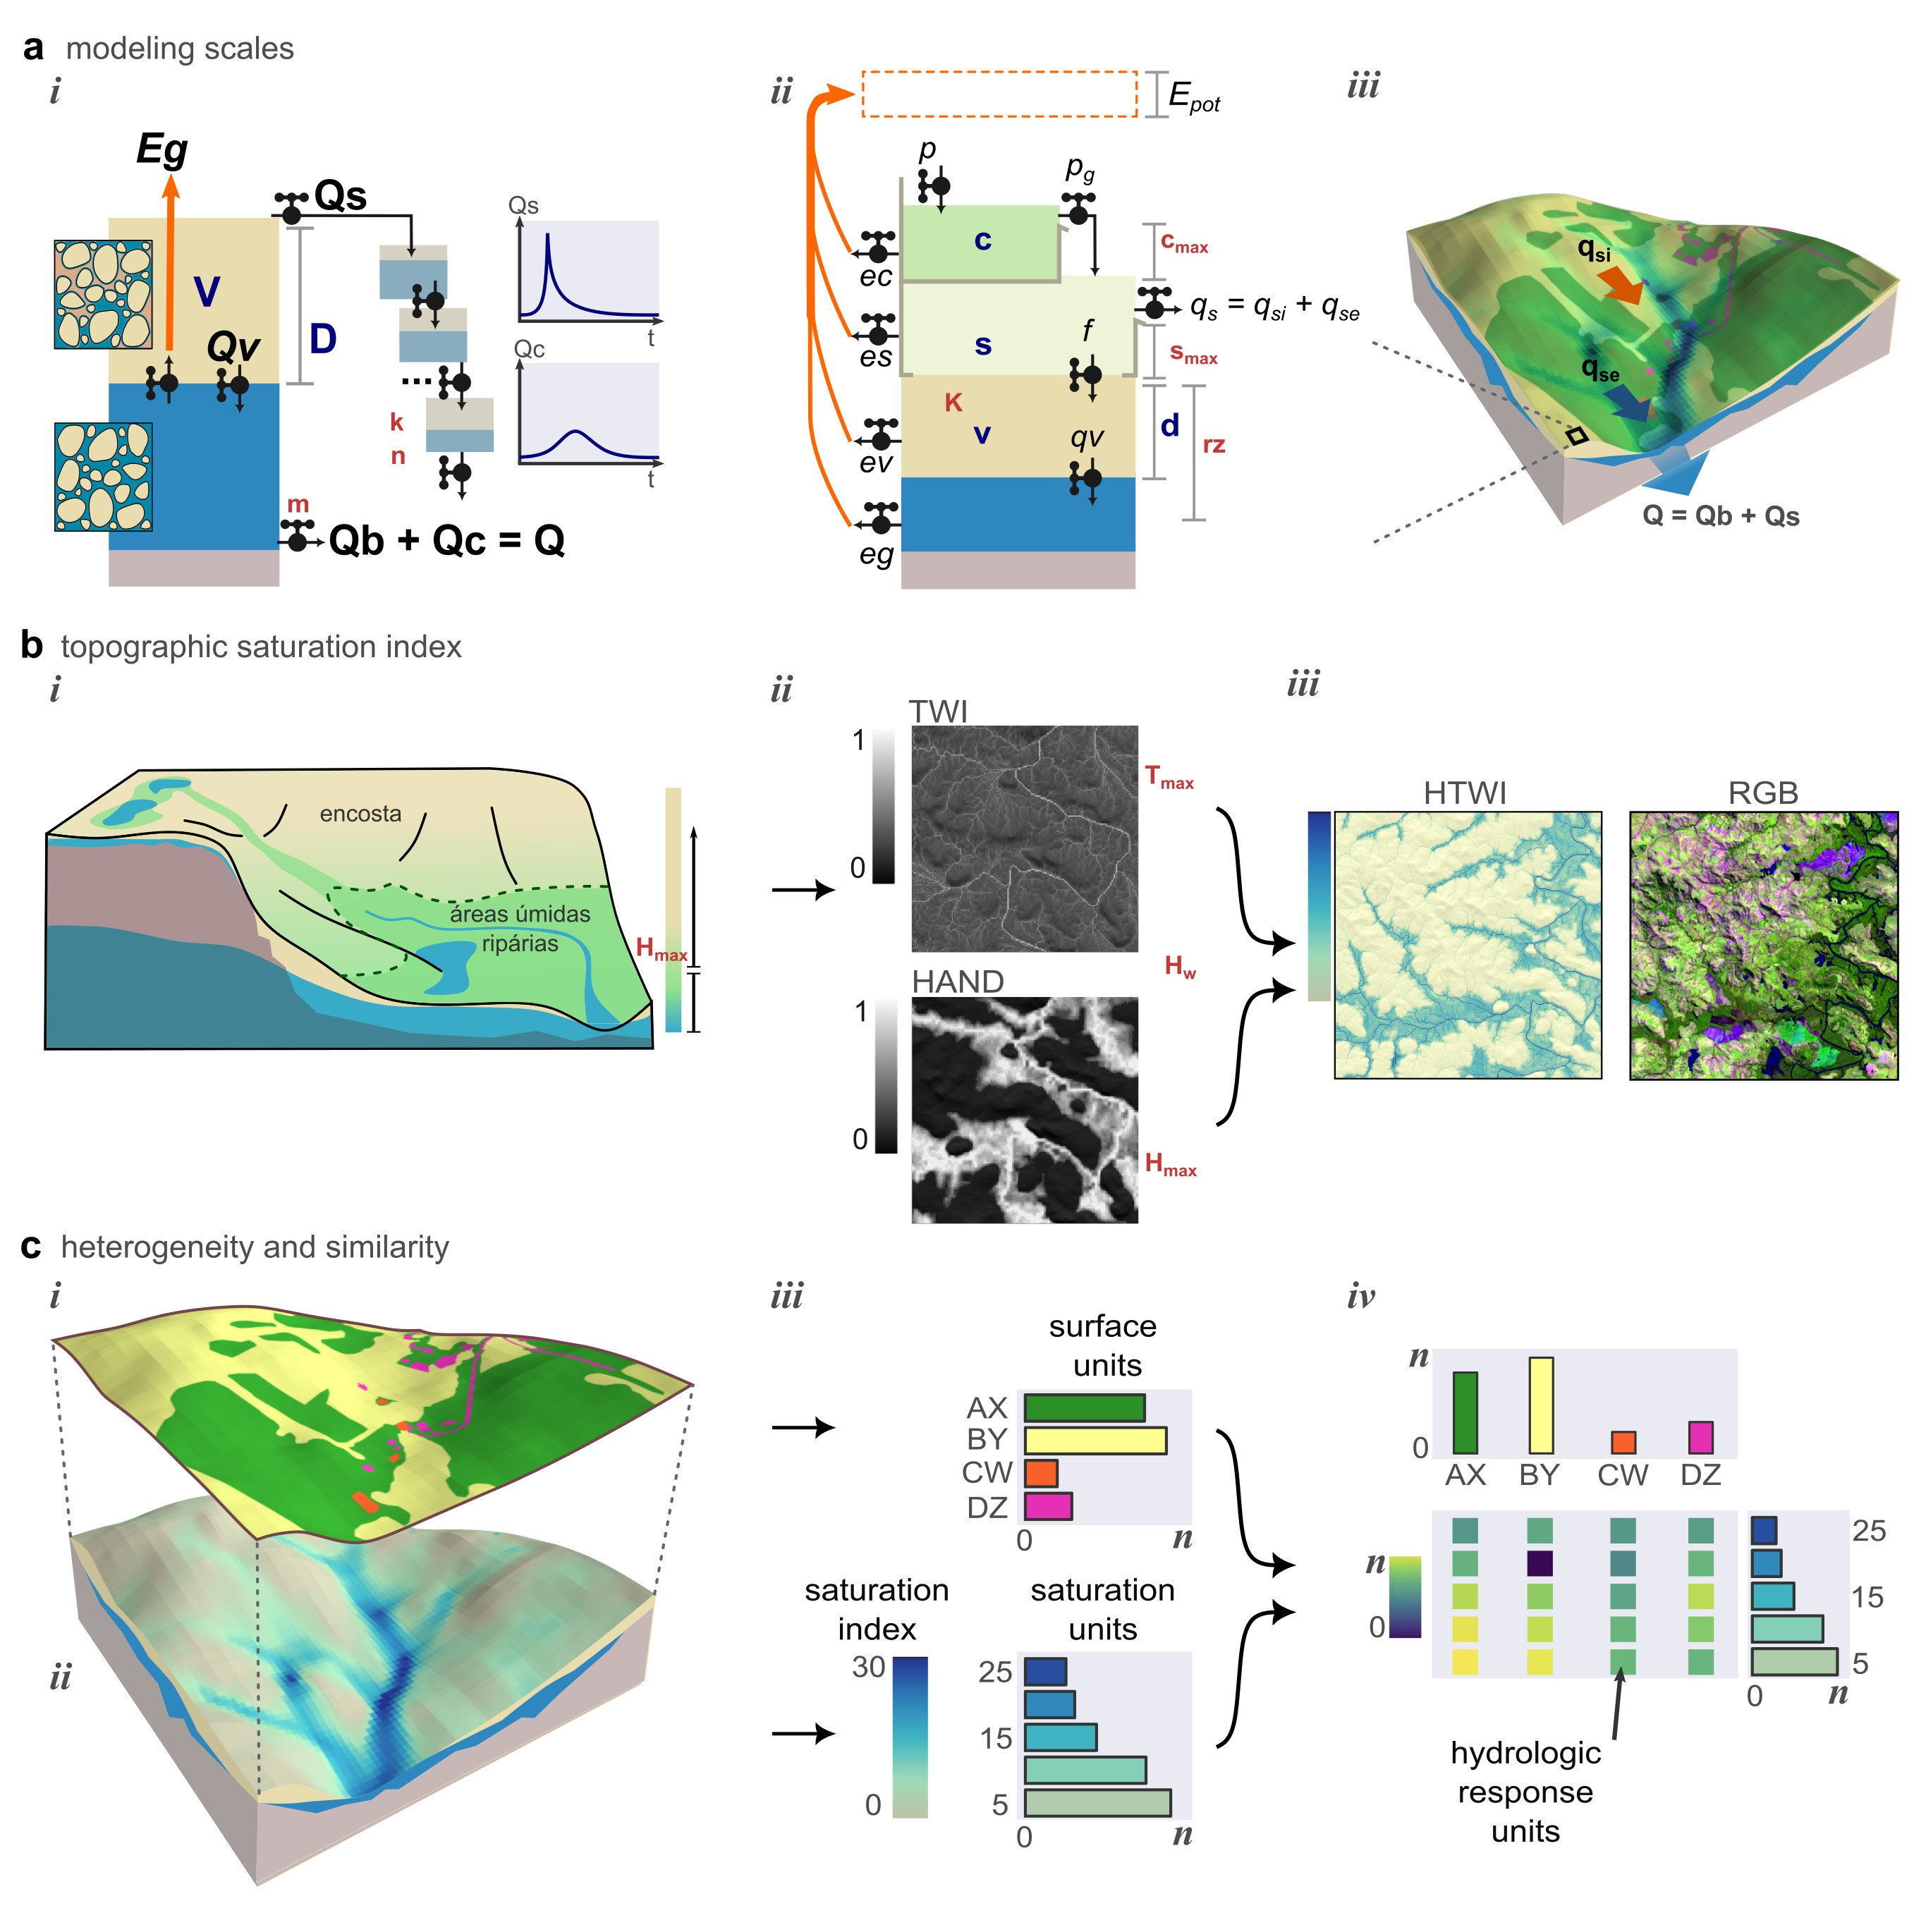
\includegraphics[width=0.98\linewidth]{figs/fig_plans_en.jpg}		
\caption[The \gls{model} \texttt{PLANS}]
{\textbf{---\;The \gls{model} \texttt{PLANS}.} The \gls{model} is a tailored version of \texttt{TOPMODEL} designed to address the problem of expanding Nature-Based Solutions.\;\textbf{a}\;---\;Modeling scales of the \gls{model}: \gls{glob-scale} (detail \textrm{\textit{i}}); \gls{urh} scale (detail \textrm{\textit{ii}}), and; local scale, at the mesh element (detail \textrm{\textit{iii}}).\;\textbf{b}\;---\;Topographic wetness index HTWI. The \gls{tsi} is based on the \gls{hipotese} of dual separation between slope areas and riparian areas (detail \textrm{\textit{i}}). The TWI and HAND indices are normalized by fuzzy logic (detail \textrm{\textit{ii}}). A weighting between the indices generates the HTWI (detail \textrm{\textit{iii}}).\;\textbf{c}\;---\;Heterogeneity and spatial similarity: the surface layer of static variables is separated from the subsurface layer of dynamic variables (details \textrm{\textit{i}} and \textrm{\textit{ii}}); the variables at the \gls{loc-scale} are grouped into surface units and saturation units (detail \textrm{\textit{iii}}); a two-dimensional histogram, or frequency matrix, is computed to store the \gls{urh} (detail \textrm{\textit{iv}}).
}
\label{fig:hydro:plans} 		
\end{figure}

\par In the \gls{model} \texttt{PLANS}, as in \texttt{TOPMODEL}, the local distribution of water deficit in the soil is done through the \gls{downscaling} function defined in Equation \ref{eq:topmodel:d5}, using a topographic wetness index $\lambda_{i}$ as a co-variable. However, unlike \texttt{TOPMODEL}, the only \gls{hipotese} fundamentally defended by the \gls{model} in this aspect is the linear relationship that the \gls{scaling-func} implies, which allows testing other topographic indices beyond the \acrshort{atwi} (Figure \ref{fig:hydro:plans}\textbf{b}). This relaxation of the hypotheses of the classic \gls{model} was primarily motivated by the practical need to address the problem of expanding \acrshort{nbs} in Brazil, a country with a wide heterogeneity of soils and landscapes, including tropical soils that are much deeper than those observed in temperate or subtropical climates. Another motivation, of a conceptual nature, is grounded in the empirical observations presented by Crave \& Gascuel-Odoux (1997) \cite{Crave1997a} regarding the distribution of saturated areas in a small watershed in France (1.3 km²), with soils varying from 40 cm to 2 meters in depth. In the study, the authors report a weak correlation between local soil saturation and the \acrshort{atwi}, as well as the relative immobility of the saturation patch at the valley bottom, largely refuting the underlying \gls{teoria} of \texttt{TOPMODEL}. On the other hand, they show that the soil saturation at sampled points $i$ has an inverse relationship with the \textit{altitude difference} $\Delta Z_{i, o}$, or height $\text{H}_{i, o}$, relative to the nearest water outcrop $o$. This inverse relationship holds up to a certain height threshold $\text{H}_\text{max}$, beyond which saturation exhibits a relatively uniform range of values. Given these observations, the authors suggest that in basins with relatively deep and well-drained soils, the landscape divides into two parts: the drier headwater region and the wetter riparian region (Figure \ref{fig:hydro:plans}\textbf{b}, detail \textit{i}). Keeping other variables constant, the separation between these two regions is reasonably delineated by the height threshold $\text{H}_\text{max}$ above the valley bottom.

\par This same topographic wetness index, referred to as \textbf{\gls{hand}}\footnote{The acronym HAND stands for \say{Height Above the Nearest Drainage}.}, was articulated ten years later by Rennó \textit{et al.} (2008) \cite{Renno2008a}, who demonstrated its effectiveness in mapping wet areas in the Amazon. However, the differentiating factor of the study by Rennó \textit{et al.} (2008) is that the authors organized the computational method to obtain the \acrshort{ahand} by applying geoprocessing techniques to \acrshort{adem}. In general terms, the technique involves initially establishing a map of the drainage network, which can be done using a drainage initiation threshold $H_{\alpha}\;[\text{L}^2]$, representing the minimum area for water to outcrop in the soil. Thus, for each mesh element $o$ in the drainage network, their respective altitudes $Z_{o, i}$ and drainage areas (basins) are obtained. Finally, the local \acrshort{ahand} $\text{H}_i$ in each basin area is calculated by the difference between the local altitude $Z_{i}$ and the altitude of the nearest drainage $Z_{o, i}$. The result is, therefore, a normalized \acrlong{adem} such that the zero altitude is always the level of the nearest river, stream, or valley bottom. The derivation of \acrshort{ahand} through geoprocessing has led to new applications, such as mapping flood risk of major rivers, since the higher one is above a river channel, the greater the safety \cite{Nobre2016a}. It becomes evident, however, that the value of \acrshort{ahand} is highly sensitive to the initially established drainage map or area threshold $H_{\alpha}$, making applications for mapping floods of major rivers (macro-drainage) very different from mapping soil saturation (micro-drainage).

\par Thus, the approach adopted in the \gls{model} \texttt{PLANS} encourages that the topographic wetness index $\lambda_i$ be obtained through fuzzy logic combinations between the \acrshort{atwi} and the \acrshort{ahand}, resulting in the index termed \textit{HAND-enhanced TWI}, or the \acrshort{atwi} enhanced by the \acrshort{ahand} (\texttt{HTWI}), illustrated in detail \textit{iii} of Figure \ref{fig:hydro:plans}\textbf{b}. This approach was actually suggested tangentially by Quinn \textit{et al.} (1991) \cite{Quinn1991b} to differentiate between ephemeral and perennial drainage regions, but concerning different flow accumulation methods. The proposed index, in this line, retains the characteristic of the \acrshort{atwi} in increasing the saturation of the landscape from upstream to downstream, but makes this effect relatively more pronounced near the \gls{sat_areas} than on drier slopes. The map is initially calculated by the fuzzy normalization of both variables, requiring the establishment of upper thresholds for each (Figure \ref{fig:hydro:plans}\textbf{b}, detail \textit{ii}). For the \acrshort{atwi}, the normalization is ascending:
\begin{linenomath*}
\begin{equation}
\label{eq:plans:ftwi}
\tilde{\text{T}}_i = \texttt{MIN}(\text{T}_i/\text{T}_\text{max},\; 1) \quad \forall \; i
\end{equation}
\end{linenomath*}
Where  $\text{T}_i\;[-]$ is the local \acrshort{atwi}; $\text{T}_\text{max}\;[-]$ is the upper threshold of the \acrshort{atwi}, and; $\tilde{\text{T}}_i\in \{0,1\}\;[-]$ is the normalized local \acrshort{atwi}. In the case of the \acrshort{ahand}, the normalization is descending:
\begin{linenomath*}
\begin{equation}
\label{eq:plans:ahand}
\tilde{\text{H}}_i = \texttt{MAX}(1 - \text{H}_i/\text{H}_\text{max},\; 0) \quad \forall \; i
\end{equation}
\end{linenomath*}
Where  $\text{H}_i\;[-]$ is the local \acrshort{ahand}; $\text{H}_\text{max}\;[-]$ is the upper threshold of the \acrshort{ahand}, and; $\tilde{\text{H}}_i\in \{0,1\}\;[-]$ is the normalized local \acrshort{ahand}. Thus, the \texttt{HTWI} is determined by the weighted average between these normalized variables and scaled back to the original range of the \acrshort{atwi}:
\begin{linenomath*}
\begin{equation}
\label{eq:plans:htwi}
\text{HT}_{i} = \text{T}_\text{max} \frac{\tilde{\text{T}}_i + H_w \tilde{\text{H}}_i}{1 + H_w} \quad \forall \; i
\end{equation}
\end{linenomath*}
Where $\text{HT}_{i}\in \{0,\text{T}_\text{max}\}\;[-]$ is the \texttt{HTWI}, and; $H_w\;[-]$ is a positive dimensionless factor or weight reflecting the dominance of the \acrshort{ahand} over the \acrshort{atwi}. The \gls{teoria} embedded in the derivation of \texttt{HTWI} is that there exists a spectrum of hydrological landscapes that extends from the total prevalence of shallow soils and dynamic saturated areas (total dominance of \acrshort{atwi} over \acrshort{ahand}) to the total prevalence of deep soils and static saturated areas (total dominance of \acrshort{ahand} over \acrshort{atwi}), with intermediate alternatives between these extreme situations. The dominance of one over the other is regulated by the weight $H_w$, while the mobility of saturated areas is regulated by the thresholds $\text{T}_\text{max}$ and $\text{H}_\text{max}$. In the special case where $H_w = 0$, the \texttt{HTWI} is identical to the \acrshort{atwi} truncated at $\text{T}_\text{max}$. This generalized topographic wetness index, adjustable for any landscape, introduces three additional \gls{parameters} into the model\footnote{In fact, when considering the drainage area threshold $\text{H}_{\alpha}$ for defining the \acrshort{ahand}, there are four additional \gls{parameters}.}, an epistemological cost that the authors deemed acceptable given the practical need to model hydrological processes in the diverse environments of Brazil. One way to reduce uncertainties in the subsequent distribution of \gls{parameters} might be to pre-condition the \textit{prior} distribution with other spatial variables obtained from remote sensing, such as moisture indices, surface temperature, or simply short-wave infrared reflectance, as illustrated in Figure \ref{fig:hydro:topo}\textbf{a}.

\par Another difference of the \gls{model} \texttt{PLANS} compared to \texttt{TOPMODEL} is the representation of surface heterogeneity (Figure \ref{fig:hydro:plans}\textbf{c}). The classic version of \texttt{TOPMODEL} was developed assuming that the surface is homogeneous, which makes sense in the Crimple Beck watershed in England, a rural area dominated by pastures for livestock. However, a \gls{model} designed to address the problem of expanding Nature-Based Solutions must not only represent the soil and its cover in heterogeneous situations but also enable the simulation of alternative cover scenarios to assess the positive or negative impact of a given expansion policy. For instance, the \gls{model} should be able to inform whether there is a difference in the behavior of the hydrological \gls{system} between reforestation in different parts of the landscape. This requirement is recognized by Gao \textit{et al.} (2015) \cite{Gao2015a}, which motivated them to implement a distributed version of \texttt{TOPMODEL} to evaluate hydrological impacts of land use and cover change. The \gls{model} \texttt{PLANS}, on the other hand, utilizes a semi-distributed approach, collapsing the \gls{loc-scale} into an intermediate \gls{urh} scale (Figure \ref{fig:hydro:plans}\textbf{a}, detail \textit{ii}). This process is accomplished through the cross-tabulation of surface units (similar patches of soil and vegetation) with saturation units (regular intervals of the topographic wetness index)\footnote{Although the soil and vegetation maps are maintained as \gls{input-data} for the \gls{model}, it is important to note that these maps are also the result of a \gls{scalab} process of other local variables. For example, the vegetation and land use classes provided in the annual maps published by Souza \textit{et al.} (2020) \cite{Souza2020a}, used in the \gls{model} \texttt{PLANS}, were derived from groupings of spectral reflectance and band indices from orbital scene data using machine learning.} (Figure \ref{fig:hydro:plans}\textbf{c}, details \textit{i}, \textit{ii}, and \textit{iii}). This tabulation ultimately results in a two-dimensional histogram, or \textbf{frequency matrix}, which specifies the area prevalence of each \gls{hydro-response} unit in the spatial region of interest\footnote{The propagation of flow to a given river section, therefore, must be conducted by specifying the prevalence of each response unit in the area of interest basin, which may or may not approximate the prevalence of the total region. This approach, thus, allows for evaluating the final flow in multiple basins of interest.}. As illustrated in detail \textit{iv} of Figure \ref{fig:hydro:plans}\textbf{c}, the columns represent the histogram of the \gls{tsi} in each surface unit. The rows of the matrix, on the other hand, are similar in terms of saturation, which readily facilitates the determination of local deficit through the \gls{downscaling} function of the \gls{model}.

\section{The paradigm of connectivity}

\par In this chapter, I organized the current twists in \gls{hydrology} since the International Hydrological Decade, that is, from the 1960s onward. On one hand, in the experimental front, the \gls{age_inf} faced its ultimate crisis with the rise of a new \gls{paradigma} that reaffirms the differentiation and uniqueness of \gls{hydro-response} mechanisms as functions of climate, topography, soils, vegetation, etc. On the other hand, in the realm of modeling, the advent of digital computers paved the way for ontologically diverse methods, such as \gls{sys-dyn}, vector fields, and statistical models, with the first two based on the theoretical description of processes and the last solely based on empirically obtained data.

% figure
\begin{figure}[t!] 
\centering				
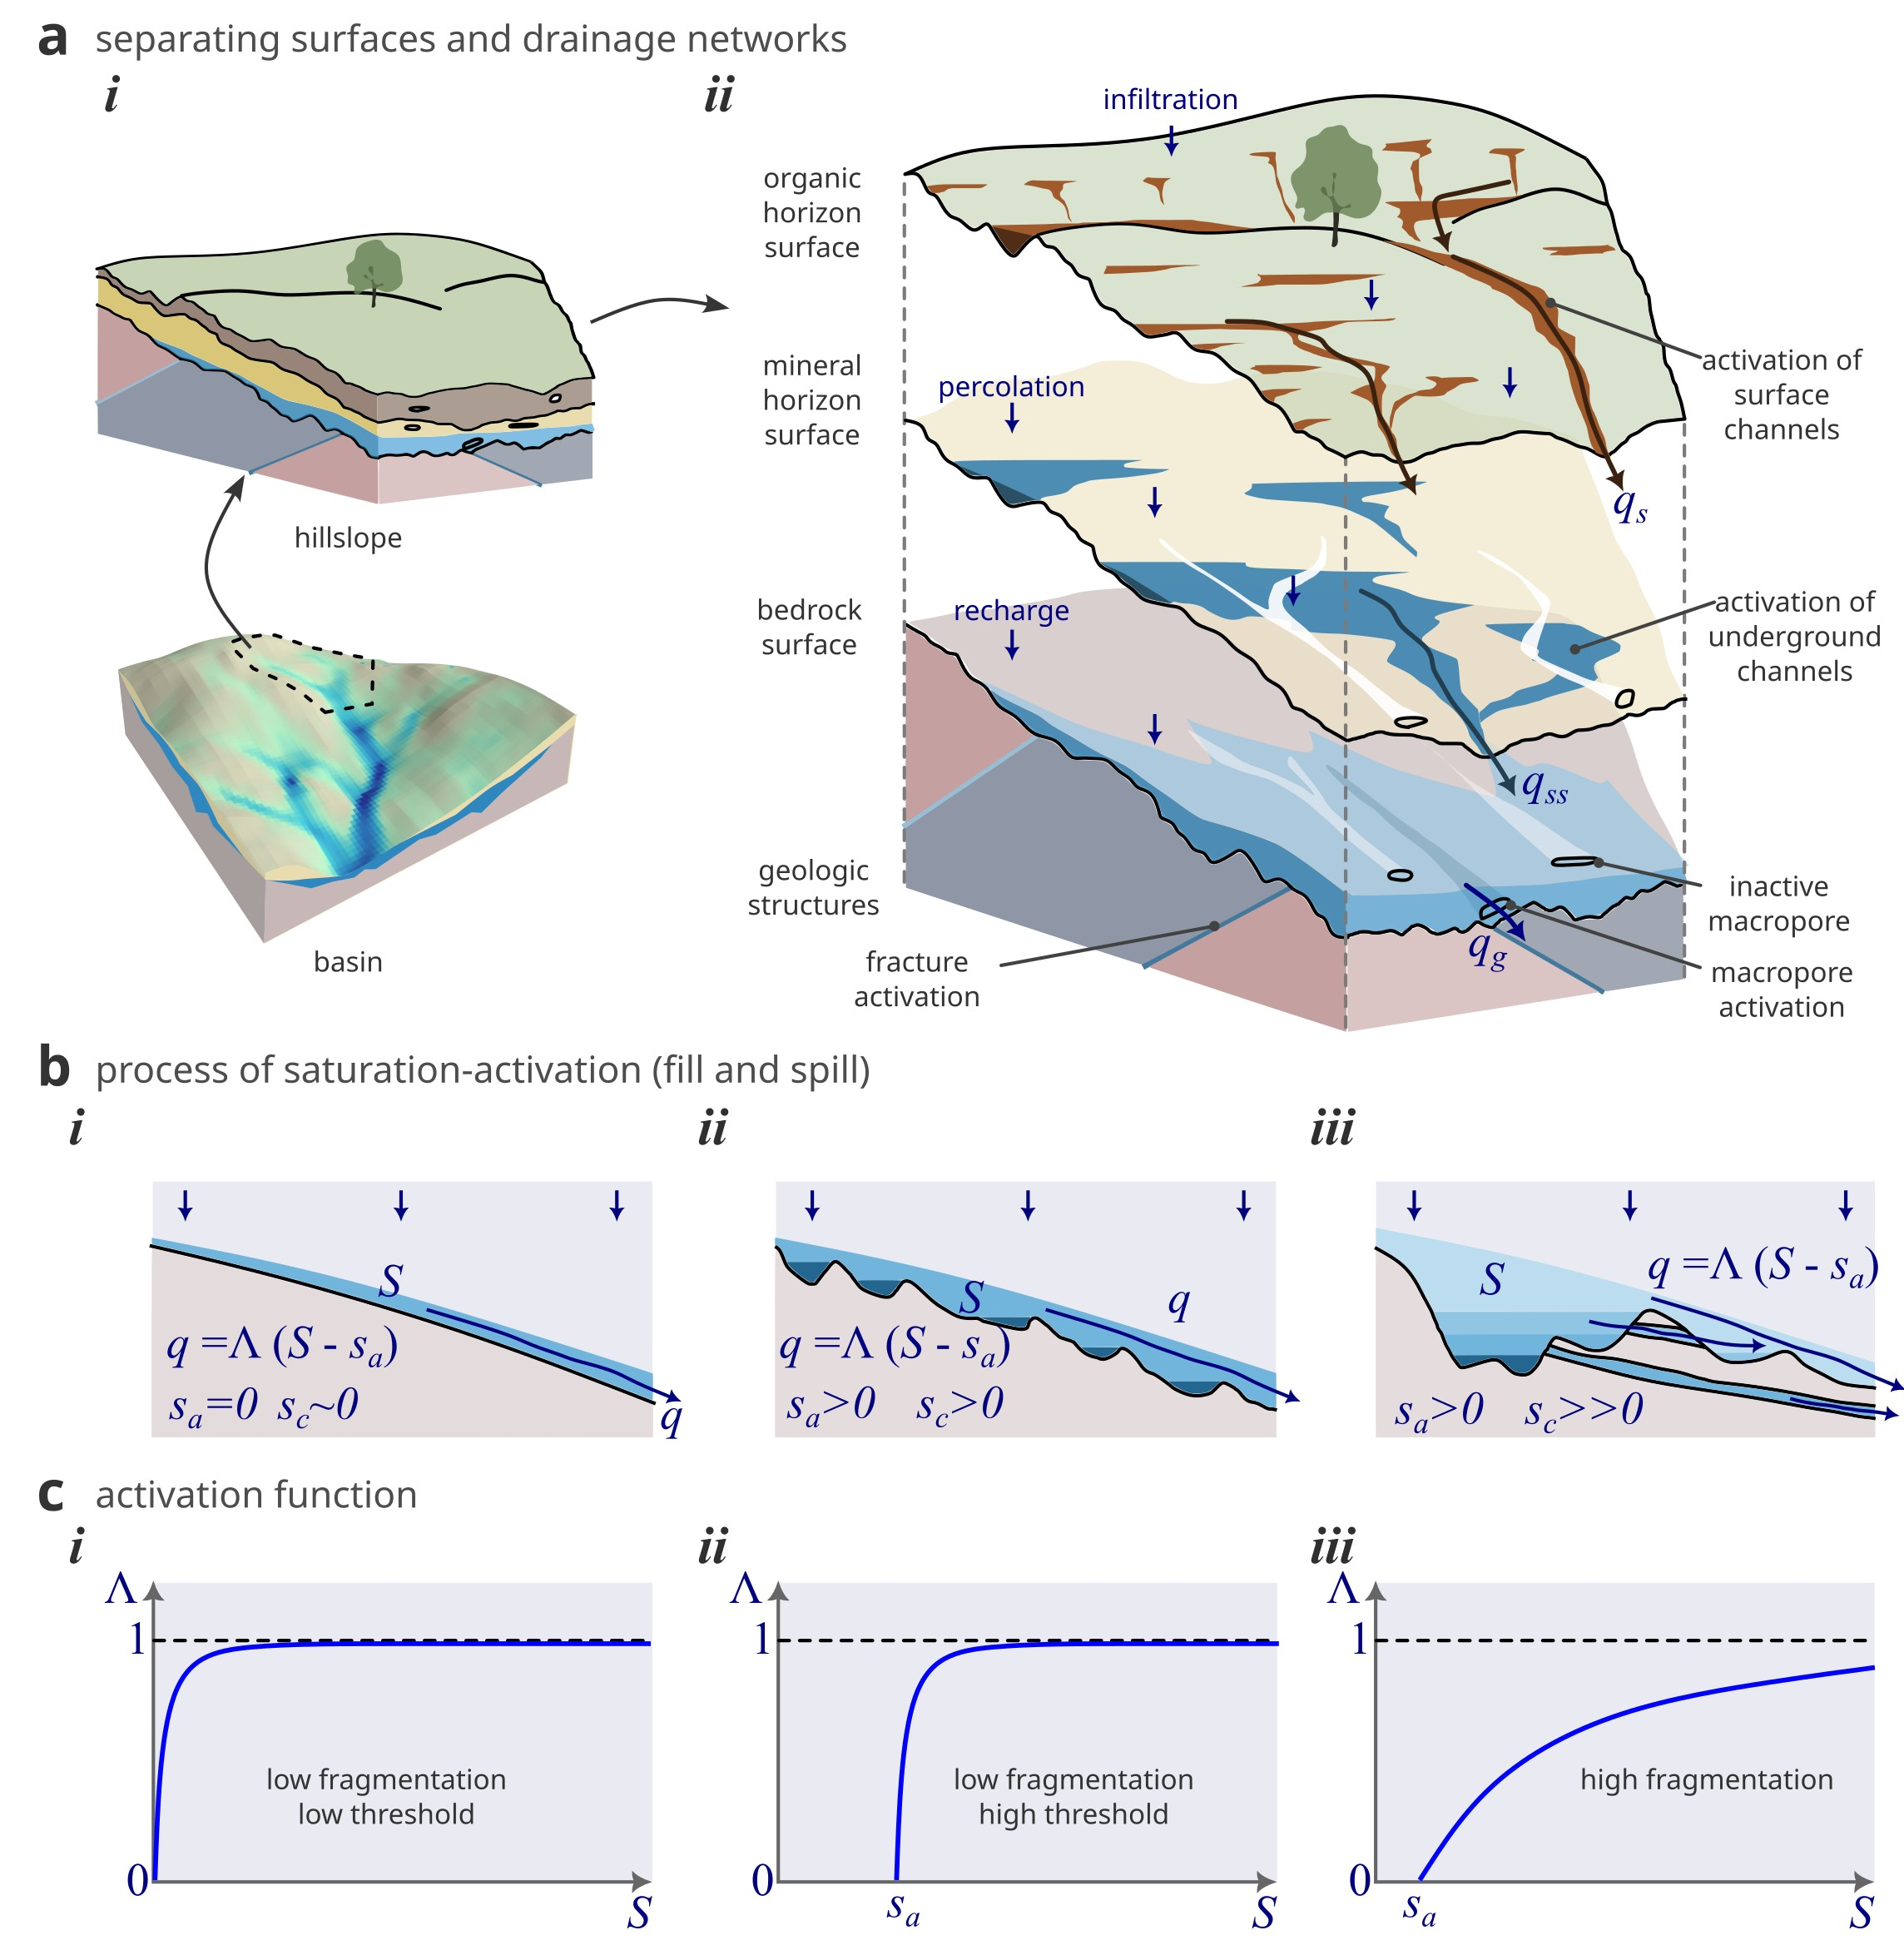
\includegraphics[width=0.98\linewidth]{figs/fig_connect_en.jpg}		
\caption[The connectivity paradigm]
{\textbf{---\;The connectivity paradigm.} The \gls{conect-theory} proposed by Jeffrey McDonnell and colleagues presents a unifying and revolutionary potential in \gls{hydrology}.\;\textbf{a}\;---\;The \gls{percept-model} is based on the principle that all hydrological responses are consequences of the same phenomenon. The vertical \gls{perm_trans} create \gls{sepsurf}. Thus, the network of channels on these surfaces can eventually become saturated and activated. Interactions also occur from bottom to top when a layer becomes saturated enough to interfere with the percolation process of the layer immediately above.\;\textbf{b}\;---\;The \gls{fillspill} occurs due to the topology of the channel network that drains the separating surface at various nested scales. The surface can be fully connected (detail \textrm{\textit{i}}) or require an initial \gls{activ-level} $s_a$ (detail \textrm{\textit{ii}}). A surface with high fragmentation $s_c$ offers multiple incrementally activated drainage networks, attenuating the response signal (detail \textrm{\textit{iii}}).\;\textbf{c}\;---\;The \gls{func-activ} $\Lambda$ can be modeled in terms of a saturation process that approaches the potential maximum flux $S - s_a$ as the surface saturates, that is, $\Lambda \rightarrow 1$.    
}
\label{fig:connnect} 		
\end{figure}

\par As new scientific paradigms do not establish themselves by being perfect, but by being better than the competition, both approaches that have settled in the field are not free from problems. In the case of experimental research, the \gls{paradigma} of differentiation encountered empirical paradoxes involving the rapid mobilization of old water and the diversity of geochemical signatures, which are difficult to explain by the mechanisms articulated by Dunne's systematization (1983) \cite{Dunne1983}. Furthermore, the experimental research program is essentially a catalog of the \gls{hydro-response} mechanisms of each unique watershed. Even though the catalog can be detailed and endlessly expanded, this operational mode does not contribute to a unifying scientific \gls{teoria} \cite{Mcdonnell2003a}. In the case of modeling, crises have affected the various approaches, giving rise to two main inescapable epistemological problems in hydrological modeling: the equifinality problem and the \gls{scale_problem} \cite{Beven1996a}. Although different, these problems are interconnected, resulting in inexorable epistemic uncertainties that hang over model results. The imperative of these epistemic problems, while overshadowing the vector field approach (forcing its proponents to appeal to pragmatic advantages), has shed new light on the ontology of \gls{sys-dyn}, making it useful for estimating uncertainties through the application of low-cost computational \gls{models-semid}.

\par That said, I will conclude the chapter by articulating the recent revolutionary ideas of Jeffrey McDonnell and colleagues, who have sought over the past two decades to pave the way for a new unifying \gls{paradigma} in \gls{hydrology}. These ideas have a direct impact on the application of hydrological models in the context of zero-order basins, making their assimilation and articulation in future versions of the \gls{model} \texttt{PLANS} of utmost importance. Although widely published, McDonnell's synthesis can be traced through three articles separated by intervals of approximately ten years: McDonnell (2003) \cite{Mcdonnell2003a}; McDonnell (2013) \cite{Mcdonnell2013}, and; McDonnell \textit{et al.} (2021) \cite{mcdonnell2021}.

\par Initially, McDonnell (2003) demonstrates the increasing disconnect between hydrological models and evidence, highlighting that the mechanisms from the International Hydrological Decade are based on assumptions that fail to explain the \gls{old_water_paradox}. Essentially, he argues that evidence points to both a greater separation between well-drained slopes and \gls{sat_areas}, as well as a greater influence of \gls{bedrock_topo} on the outcropping of groundwater. Together, these two factors produce rapid translational flow of pre-event (old) water with diverse geochemical signatures. In the field of modeling, McDonnell (2003) asserts that the appropriate ontology for the new challenges is \gls{sys-dyn}, not merely for convenience, but because it allows for the representation of the different compartments of the \gls{zero-basin}, primarily slopes and riparian zones, and guarantees exploratory experiments at a low computational cost. As highlighted in the chapter's epigraph, \gls{sys-dyn} reaffirms itself as an ontological \gls{paradigma} that is both intuitive and objective for understanding and learning about environmental systems.

\par The second step by McDonnell (2013) is to propose the \textbf{\gls{conect-theory}} as the definitive explanation for both the hydrological processes systematized by Dunne (1983) and the (not so) recent findings regarding the \gls{old_water_paradox}. Initially reported in Meerveld \& McDonnell (2006) \cite{Meerveld2006b} to explain processes in a specific experimental basin, McDonnell generalizes his concepts, treating it as a revolutionary and unifying \gls{teoria} that seeks to resolve the crisis established in the field. McDonnell proposes this \gls{teoria} from a question that sounds like heresy: could the rapid and slow responses of basins all be \textit{the same phenomenon}?

\begin{adjustwidth}{100pt}{0pt}
\medskip
\small (...) the simple premise that all runoff processes are the same opens up new avenues to explore: Is there common emergent behaviour across all runoff types? -- Jeffrey McDonnell (2013, p. 4110) \cite{Mcdonnell2013}.
\medskip
\end{adjustwidth}

\par This provocative question leads him to demonstrate that any \gls{system} formed by networks of small channels can be modeled by the \textbf{Percolation Theory}, a mathematical branch of Network Theory\footnote{Unlike scientific theories, which require empirical evidence to be corroborated, mathematical theories are based on axioms and \gls{infer-dedu}.} \cite{Janzen2015a}. According to this \gls{teoria}, flow occurs through a network as long as there are connections between the nodes. In the case of a \gls{zero-basin}, in the physical world, the different parts of the \gls{system} each function as a network of small reservoirs connected by small channels (open or closed, macroscopic or microscopic). Here, the relevance of two key concepts from the \gls{teoria} arises: (1) the \textbf{\gls{sepsurf}} between compartments, created by the transition of vertical permeability between soil horizons, and; (2) the \textbf{\gls{activ-threshold}} of the compartment, which primarily arises from the heterogeneity of the separating surface.

\par A clear example of this is the generation of flash floods when the soil's infiltration capacity is insufficient. Typically, the level of surface depressions needs to reach an \gls{activ-threshold}, at which point some surface depressions connect for the first time and start to spill water downhill. With more rain, the puddles continue to fill until a point is reached where all the incoming rainwater can flow downhill. The speed at which the connection occurs depends on the heterogeneity of the soil surface: a smooth surface is much more connected than a rough surface.

\par Although it may seem obvious, McDonnell suggests that the \textbf{\gls{fillspill}}\footnote{A loose translation of the English term \textit{fill and spill}.} that generates flash floods occurs in all subsurface layers where vertical water flow encounters a transition in permeability, including the relatively impermeable bedrock layer (Figure \ref{fig:connnect}\textbf{a}). The only difference in the subsurface environment is that the network of channels is composed of the micro and macropores of the immediately overlying horizon. In this context, the \gls{teoria} even allows for relatively small amounts of event water (new water) to activate the connection between pockets of stored water from before the event (old water). The pressurization in the saturated zone, along with the formation of natural siphons in the subsurface, eventually expels \textit{more} water than what entered, generating a negative mass balance on the slope and a hysteretic behavior of flow pulses. Finally, when a separating surface becomes sufficiently saturated, it propagates this effect from bottom to top, causing saturation of the upper layer, thereby creating conditions analogous to the \gls{sat_areas} we observe on the surface.

\par Finally, in their third move, McDonnell \textit{et al.} (2021) articulate how to approach the \gls{conect-theory} in the context of modeling, considering the \gls{scale_problem}. Again, \gls{sys-dyn} is presented as the appropriate ontology for representing the \gls{sys-target}, emphasizing the explicit definition of the scale of interest, identifying the saturation-activation processes that manifest at the chosen \gls{model-scale}. The authors' \gls{hipotese} is that saturation-activation processes occur at all scales; however, the signals emitted by smaller scales are progressively masked by saturation-activation at larger scales (Figure \ref{fig:connnect}\textbf{b}). For example, while at the scale of zero-order basins the \gls{fillspill} is primarily dictated by topography, soil, and vegetation, this signal fades at the scale of higher-order basins, with the saturation-activation effects of the river drainage \gls{system} and flooding of the plains becoming more dominant. Thus, experimental and modeling research must explicitly question what scale is being addressed and which critical saturation-activation processes are necessary to understand the \gls{sys-target}. Relatively simple (yet objective) \gls{sys-dyn} models can capture this knowledge, formalizing the main \gls{hipotese} of the \textbf{\gls{func-activ}}, which takes the following general form:
\begin{linenomath*}
\begin{equation}
\label{eq:conect:general}
Q_a = 
\begin{cases} 
    0 & \text{if } \quad S \leq s_a\\
    \Lambda \cdot (S - s_a) & \text{if } \quad S > s_a
\end{cases}
\end{equation}
\end{linenomath*}
Where $Q_a\;[\text{L}\text{T}^{-1}]$ is the activation flow of the reservoir with level $S\;[\text{L}]$; $s_{a}\;[\text{L}]$ is the \textbf{\gls{activ-level}} of the reservoir, and; $\Lambda \;[\text{T}^{-1}]$ is the \textbf{\gls{func-activ}} of the reservoir, to be defined based on the \gls{aux-hyp} of the \gls{model}. In the previous chapter, during the development of the hydrological \gls{model} prototype, I applied these exact principles for the quick response flow $R$ of the surface reservoir $S_1$ (see Section \ref{sec:systems:model}). Equation \eqref{eq:fast_response} has exactly the same structure as Equation \eqref{eq:conect:general}, with $\Lambda = c$, a runoff coefficient defined between 0 and 1 obtained from a \gls{func-activ} with the following structure (Figure \ref{fig:connnect}\textbf{c}):
\begin{linenomath*}
\begin{equation} 
	\label{eq:conect:af}
	\Lambda = \frac{(S - s_a)}{(S - s_a) + s_c} \frac{1}{\Delta t}
\end{equation}
\end{linenomath*}
Where $s_{a}\;[\text{L}]$ is the \gls{activ-level} of the reservoir, and;  $s_{c}\;[\text{L}]$ is the \textbf{\gls{frag-level}} of the reservoir. This function, when coupled into \eqref{eq:conect:general}, implies that the outflow $Q_a$ caused by activation asymptotically approaches the potential maximum flux ($S - s_a$) as the reservoir level $S$ increases, because higher levels increasingly activate the drainage network. In other words, $\lim _{S \to \infty} \Lambda= 1$ in \eqref{eq:conect:af} and $\lim _{S \to \infty} Q_a = (S - s_a)/ \Delta t$ in \eqref{eq:conect:general}. The \gls{frag-level} $s_c$ is a parameter that plays the role of regulating the speed of this process, serving as a measure of inverse connectivity (the higher, the less connected the reservoir is). The physical interpretation of the \gls{frag-level} is the level $S$ necessary to reach half of the potential maximum flux. The \textbf{Michaelis-Menten equation} \cite{Johnson2011a}, which describes an enzyme saturation process, coincidentally has an identical structure, making it a notable \gls{homology}. Another identical structure is the equation from the \textbf{CN method}, empirically proposed based on the results of Mockus (1949) \cite{mockus1949}. The difference in this case is that the creators of the CN method express the level $S$ in terms of accumulated rainfall $P$, which is only valid for a surface reservoir with unlimited capacity. The \gls{frag-level}, in this regard, is expressed in terms of a dimensionless connectivity coefficient, such that $s_c = (1000/\text{CN}) - 10$. Such homologies and theoretical explanations of old empirical adjustments outline the contours of a legitimately revolutionary scientific \gls{teoria}. $\blacksquare$

\clearpage

\section{Chapter summary} \label{sec:hydro:summary}

\par In this chapter, I provided a historical and theoretical overview of the evolution of hydrological models, highlighting the main changes in approaches and scientific paradigms. Beginning with slopes, where hydrological processes start, I explored the transition from Horton’s infiltration model to more complex concepts that incorporate climatic, geomorphological, and biological variability. I also analyzed the limitations faced by modern computational models, such as scale and equifinality problems, culminating in the \gls{conect-theory}, which proposes an innovative integration of surface and subsurface flow processes.

\begin{itemize}
    \item[$\blacksquare$] \textbf{Slopes are where it all begins.} Rapid hydrological responses (floods) and slow responses (recessions) begin with rain on the slopes or zero-order basins. Simplifying this complexity can lead to inadequate models, especially in the context of watershed revitalization. Therefore, it is crucial to recognize the theories regarding runoff generation at this scale.
    
    \item[$\blacksquare$] \textbf{The Age of Infiltration.} During the mid-20th century, the hegemony of Horton’s hydrological model was established, explaining hydrological responses through the soil's infiltration capacity, separating rainfall into runoff and recharge. Although surpassed, this \gls{paradigma} elevated \gls{hydrology} from its empirical phase to a geoscience.

    \item[$\blacksquare$] \textbf{The Age of Differentiation.} With the International Hydrological Decade in the 1960s, new evidence and theories emerged that refuted Horton. This new \gls{paradigma} explores how different hydrological responses arise due to climate, topography, soils, and vegetation. In addition to floods, the roles of macropores and \gls{sat_areas} were highlighted. However, a crisis emerged with the \gls{old_water_paradox}.
    
    \item[$\blacksquare$] \textbf{Inevitable Limitations.} Digital computers enabled hydrological models, divided into two families: data-driven (predictions) and process-based (explanations). \gls{sys-dyn} exposed the limitations imposed by equifinality and scale problems, which persisted even with attempts to resolve them using vector field-based models.
    
    \item[$\blacksquare$] \textbf{Information Scaling.} The \gls{scale_problem} refers to the difficulty of reconciling the natural scales of hydrological processes with observational and conceptual scales. The solution is the \gls{scalab} of information. The \texttt{TOPMODEL} achieves this by scaling soil saturation with the \texttt{TWI} index. The \texttt{PLANS} combines \texttt{HAND} and \texttt{TWI} to scale saturation across different landscapes and instantiate \gls{urh}.
    
    \item[$\blacksquare$] \textbf{The Connectivity Theory.} Jeffrey McDonnell proposes a unifying and revolutionary \gls{teoria} suggesting that surface and subsurface flows are manifestations of a single phenomenon: the saturation-activation of channel networks. In light of the inescapable limitations, \gls{sys-dyn} is deemed the best alternative to model this \gls{teoria}.
    
\end{itemize}


\end{document}